\documentclass[twoside]{book}

% Packages required by doxygen
\usepackage{fixltx2e}
\usepackage{calc}
\usepackage{doxygen}
\usepackage[export]{adjustbox} % also loads graphicx
\usepackage{graphicx}
\usepackage[utf8]{inputenc}
\usepackage{makeidx}
\usepackage{multicol}
\usepackage{multirow}
\PassOptionsToPackage{warn}{textcomp}
\usepackage{textcomp}
\usepackage[nointegrals]{wasysym}
\usepackage[table]{xcolor}

% Font selection
\usepackage[T1]{fontenc}
\usepackage[scaled=.90]{helvet}
\usepackage{courier}
\usepackage{amssymb}
\usepackage{sectsty}
\renewcommand{\familydefault}{\sfdefault}
\allsectionsfont{%
  \fontseries{bc}\selectfont%
  \color{darkgray}%
}
\renewcommand{\DoxyLabelFont}{%
  \fontseries{bc}\selectfont%
  \color{darkgray}%
}
\newcommand{\+}{\discretionary{\mbox{\scriptsize$\hookleftarrow$}}{}{}}

% Page & text layout
\usepackage{geometry}
\geometry{%
  a4paper,%
  top=2.5cm,%
  bottom=2.5cm,%
  left=2.5cm,%
  right=2.5cm%
}
\tolerance=750
\hfuzz=15pt
\hbadness=750
\setlength{\emergencystretch}{15pt}
\setlength{\parindent}{0cm}
\setlength{\parskip}{3ex plus 2ex minus 2ex}
\makeatletter
\renewcommand{\paragraph}{%
  \@startsection{paragraph}{4}{0ex}{-1.0ex}{1.0ex}{%
    \normalfont\normalsize\bfseries\SS@parafont%
  }%
}
\renewcommand{\subparagraph}{%
  \@startsection{subparagraph}{5}{0ex}{-1.0ex}{1.0ex}{%
    \normalfont\normalsize\bfseries\SS@subparafont%
  }%
}
\makeatother

% Headers & footers
\usepackage{fancyhdr}
\pagestyle{fancyplain}
\fancyhead[LE]{\fancyplain{}{\bfseries\thepage}}
\fancyhead[CE]{\fancyplain{}{}}
\fancyhead[RE]{\fancyplain{}{\bfseries\leftmark}}
\fancyhead[LO]{\fancyplain{}{\bfseries\rightmark}}
\fancyhead[CO]{\fancyplain{}{}}
\fancyhead[RO]{\fancyplain{}{\bfseries\thepage}}
\fancyfoot[LE]{\fancyplain{}{}}
\fancyfoot[CE]{\fancyplain{}{}}
\fancyfoot[RE]{\fancyplain{}{\bfseries\scriptsize Generated by Doxygen }}
\fancyfoot[LO]{\fancyplain{}{\bfseries\scriptsize Generated by Doxygen }}
\fancyfoot[CO]{\fancyplain{}{}}
\fancyfoot[RO]{\fancyplain{}{}}
\renewcommand{\footrulewidth}{0.4pt}
\renewcommand{\chaptermark}[1]{%
  \markboth{#1}{}%
}
\renewcommand{\sectionmark}[1]{%
  \markright{\thesection\ #1}%
}

% Indices & bibliography
\usepackage{natbib}
\usepackage[titles]{tocloft}
\setcounter{tocdepth}{3}
\setcounter{secnumdepth}{5}
\makeindex

% Hyperlinks (required, but should be loaded last)
\usepackage{ifpdf}
\ifpdf
  \usepackage[pdftex,pagebackref=true]{hyperref}
\else
  \usepackage[ps2pdf,pagebackref=true]{hyperref}
\fi
\hypersetup{%
  colorlinks=true,%
  linkcolor=blue,%
  citecolor=blue,%
  unicode%
}

% Custom commands
\newcommand{\clearemptydoublepage}{%
  \newpage{\pagestyle{empty}\cleardoublepage}%
}

\usepackage{caption}
\captionsetup{labelsep=space,justification=centering,font={bf},singlelinecheck=off,skip=4pt,position=top}

%===== C O N T E N T S =====

\begin{document}

% Titlepage & ToC
\hypersetup{pageanchor=false,
             bookmarksnumbered=true,
             pdfencoding=unicode
            }
\pagenumbering{alph}
\begin{titlepage}
\vspace*{7cm}
\begin{center}%
{\Large Algorithmic Regularization Chain (A\+RC) }\\
\vspace*{1cm}
{\large Generated by Doxygen 1.8.12}\\
\end{center}
\end{titlepage}
\clearemptydoublepage
\pagenumbering{roman}
\tableofcontents
\clearemptydoublepage
\pagenumbering{arabic}
\hypersetup{pageanchor=true}

%--- Begin generated contents ---
\chapter{A\+RC Introduction}
\label{index}\hypertarget{index}{}\hypertarget{index_AR_sec}{}\section{Algorithmic Regularization (\+A\+R)}\label{index_AR_sec}
The algorithm used in this code is based on the literatures of \href{http://adsabs.harvard.edu/abs/1999MNRAS.310..745M}{\tt Mikkola \& Tanikawa (1999)} and \href{http://adsabs.harvard.edu/abs/1999AJ....118.2532P}{\tt Preto \& Tremaine (1999)}. The development of this code refers to the Chapter 2 (Mikkola) in book \href{http://www.springer.com/us/book/9781402084300}{\tt The Cambridge N-\/body Lectures}. Here the basic idea of AR is described.

The numerical simulations of gravitational N-\/body systems dynamical evolutions are frequently used in astrophysics. However, due to the singularity of two-\/body gravitational potential when these two particles become infinite close lead to the difficulty in the highly accurately integration of two-\/body bounded system with very high eccentricity. To get high accuracy of integration when two particles are very close, the time step for integration should be reduced significantly. This result in time consuming computation if number of particles is large. On the other hand, for a long-\/term integration, the total energy of the systems may be systematiclly drifted due to the numerical accuracy of integrators. Thus the sympletic methods are suggested to be used since it can keep the energy conservation for long-\/term integration.

However, the sympletic methods are difficult to be applied for gravitational systems due to the required time step (integration step) shrinking when two particle get close. Thus Mikkola \& Tanikawa (1999) and Preto \& Tremaine (1999) develop the special time transformation method based on the extended phase space Hamiltonian. The time $t$ become a general coordinate in Hamiltonian with corresponding general momentum $Pt$. The integration of the equation of motion then depends on the new differential variable $ s$. In this case, time and the motion of the system can be integrated with a fixed step size of s, which allow the usage of sympletic methods.\hypertarget{index_H_sec}{}\subsection{Hamiltonian in Extended Phase Space}\label{index_H_sec}
Defining the general coordinates as $ \mathbf{q} = \{q_i\}, (i=1,n) $ with freedom of $n$ and corresponding general momentums ad $ \mathbf{p} $, The Hamiltonian equations is\+:

(1) $ \frac{d \mathbf{q}}{d t} = \frac{\partial H}{\partial \mathbf{p}}$; $ \frac{d \mathbf{p}}{d t} = - \frac{\partial H}{\partial \mathbf{q}} $

Here the dt is used as a differetial varaible. For the propuse as we discussed above, we want to use a new variable $s$ replacing the function of time $t$. In this case, the time is treated as a new general coordinate. And the corresponding time momentum $Pt$ should be also added.

We extend the coordiantes to $ \mathbf{Q} = (t, \mathbf{q}) $ and the momentums to $ \mathbf{P} = (Pt, \mathbf{p})$ with total freedom of $2(n+1)$.

The new Hamiltonian $H'$ should also satisfy the Hamiltonian equations (1). Especially for $(t, Pt)$, we can get\+:

(2) $ \frac{d t}{d t} = \frac{\partial H'}{\partial Pt} = 1 $; $ \frac{d Pt}{d t} = - \frac{\partial H'}{\partial t} = - \frac{\partial H}{\partial t}$

From first equation of (2), we find the $H'$ linearly depend on $Pt$, thus $H'$ can be the form as $ H' = H + Pt $. The second equation indicates that the time evolution of $Pt$ is equal to the negative energy change of the system. Thus the value of $Pt$ at the time $t$ can be $-H(t)$.

We want to write Hamiltonian equations with new differetial variable $ ds$. Defining $ g(\mathbf{Q},\mathbf{P}) = \frac{dt}{ds} $, we can rewrite (1) with $ds$ and extended coordinates $(\mathbf{Q}, \mathbf{P})$ as\+:

(3) $ \frac{d \mathbf{Q}}{d s} = g(\mathbf{Q},\mathbf{P}) \frac{\partial H'}{\partial \mathbf{P}} $; $ \frac{d \mathbf{P}}{d s} = - g(\mathbf{Q},\mathbf{P}) \frac{\partial H'}{\partial \mathbf{Q}} $

However, we need to have the Hamiltonian equations the same form as original, thus we need to find another Hamiltonian $\Gamma(\mathbf{P},\mathbf{Q})$ that satisfy the Hamiltonian equations\+:

(4) $ \frac{d \mathbf{Q}}{d s} = \frac{\partial \Gamma}{\partial \mathbf{P}} $; $ \frac{d \mathbf{P}}{d s} = -\frac{\partial \Gamma}{\partial \mathbf{Q}} $

To find correct $\Gamma(\mathbf{P},\mathbf{Q})$, we go back to the Principle of least action which is used to derive the Lagrangian equations. The relation between (standard) Hamiltonian $H(\mathbf{p},\mathbf{q},t)$ and Lagrangian $L(\mathbf{p},\mathbf{q},t)$ is

(5) $ H(\mathbf{p},\mathbf{q},t) = \sum_{i=1}^n p_i \dot{q_i} - L(\mathbf{p},\mathbf{q},t) $

The Principle of least action require the action

(6) $ S = \int_{t_1}^{t_2} L(\mathbf{p},\mathbf{q},t) dt = \int_{t_1}^{t_2} \left[ \sum_{i=1}^n p_i \dot{q_i} - H(\mathbf{p},\mathbf{q},t) \right] dt $

should take the mimimum path, thus any function variation $ \delta S $ should makes $ S + \delta S$ increase. Thus when $ \delta L(\mathbf{p},\mathbf{q},t) = 0 $, this condition is satisfied. This leads to the Lagrangian equations and also the Hamitonian equations.

Here the integration takes from $ t_1 $ to $ t_2 $ and the time is used as integration variable. Now we treat $(t, Pt)$ as new coordinate and momemtum, $H'$ as new Hamitonian, and use $s$ as new integration variable. Then $S$ can be rewrited as\+:

(7) $ S = \int_{s_1}^{s_2} \left[ \sum_{i=1}^n p_i \frac{d q_i} {d s} + Pt \frac{d t}{d s} - (H(\mathbf{p},\mathbf{q},t) + Pt) \frac{d t}{d s} \right] ds = \int_{s_1}^{s_2} \left[ \sum_{i=1}^{n+1} P_i \frac{d Q_i}{d s} - H'(\mathbf{P},\mathbf{Q}) \frac{d t}{d s}\right] ds $

It is obvious that when

(8) $ \Gamma(\mathbf{P},\mathbf{Q}) = H'(\mathbf{P},\mathbf{Q}) \frac{d t}{d s} = g(\mathbf{Q},\mathbf{P}) (H(\mathbf{p},\mathbf{q},t) + Pt) $

The formula (7) become the same form as (6). Then with Principle of least action, the Hamiltonian equation (4) can be derived. We call the $ \Gamma(\mathbf{P},\mathbf{Q}) $ is the Hamiltonian in the extended phase space $ (\mathbf{P},\mathbf{Q}) $

The Hamiltonian in extended phase space $\Gamma$ is also useful for analyzing the systems where Hamiltonian $H$ explicitly depends on time and is not conserved. Since time become a coordinate in $\Gamma$, $\frac{\partial \Gamma}{\partial s}$ is zero thus $ \Gamma$ become conserved quantity. The method dealing with closed system can be used with Hamiltonian in extended phase space.\hypertarget{index_T_sec}{}\subsection{Time transformation for Separable Hamiltonian}\label{index_T_sec}
With the Hamiltonian in extended phase space, we can integrate the equation of motions with step $ ds $ by choosing a kind of $g(\mathbf{Q},\mathbf{P})$. If we choose a $g(\mathbf{Q},\mathbf{P})$ that makes the Hamiltonian $\Gamma(\mathbf{Q},\mathbf{P})$ separable for $P$ and $Q$\+:

(9) $ \Gamma(\mathbf{Q},\mathbf{P}) = a(\mathbf{P}) + b(\mathbf{Q}) $

Then explicit Leapfrog (S\+IA) integration method can be used. Preto \& Tremaine (1999) suggests to use

(10) $ g(\mathbf{Q},\mathbf{P}) = \frac{f(T(\mathbf{P})) - f(-U(\mathbf{Q}))}{T(\mathbf{P}) + U(\mathbf{Q})} $

where $ T(\mathbf{P}) = T(\mathbf{p}) + Pt $ is the extended kinetic energy and $ U(\mathbf{Q}) = U(\mathbf{q},t) $ is the extended potential energy.

The Hamiltonian becomes separable\+:

(11) $ \Gamma = f(T(\mathbf{P})) - f(-U(\mathbf{Q})) $

Then the equation of motions are\+:

(12) $ \frac{d \mathbf{q} }{d s} = f'(T(\mathbf{p})+Pt) \frac{\partial T(\mathbf{p})}{\partial {\mathbf{p}}} $; $ \frac{d t }{d s} = f'(T(\mathbf{p})+Pt) $; $ \frac{d \mathbf{p} }{d s} = f'(-U(\mathbf{q},t)) \frac{\partial U(\mathbf{q},t)}{\partial {\mathbf{q}}} $; $ \frac{d Pt}{d s} = f'(-U(\mathbf{q},t)) \frac{\partial U(\mathbf{q},t)}{\partial {\mathbf{t}}} $;

where $ f'(x) = \frac{d f(x)}{d x} $.

Since $Pt = -H(t)$, $H'=H+Pt = T(\mathbf{P}) + U(\mathbf{Q}) = 0 $. Thus during integration, $T(\mathbf{P}) \approx -U(\mathbf{Q}) $. This requires $ f(T(\mathbf{P})) - f(-U(\mathbf{Q})) \approx 0 $. With Taylor expansion, we can obtain\+:

(13) $ f(T(\mathbf{P})) = f(-U(\mathbf{Q})) + \left[T(\mathbf{P}) + U(\mathbf{Q})\right] f'(-U(\mathbf{Q})) + O\left[T(\mathbf{P}) + U(\mathbf{Q})\right]^2 $

Thus

(14) $ g(\mathbf{Q},\mathbf{P}) \approx f'(-U(\mathbf{Q})) $\hypertarget{index_logH_sec}{}\subsubsection{Logarithmic Hamintonian method (\+Log\+H)}\label{index_logH_sec}
Mikkola \& Tanikawa (1999) suggests to use the function $ f(x) = \log{x} $ (Logarithmic Hamintonian method). In this case, the time transformation based on (14) is\+:

(15) $ g(\mathbf{Q},\mathbf{P}) \approx \frac{1}{-U(\mathbf{Q})} $

Then the equation of motions can be written as\+:

(16) $ \frac{d \mathbf{q} }{d s} = \frac{1}{T(\mathbf{p})+Pt} \frac{\partial T(\mathbf{p})}{\partial {\mathbf{p}}} $; $ \frac{d t }{d s} = \frac{1}{T(\mathbf{p})+Pt} $; $ \frac{d \mathbf{p} }{d s} = \frac{1}{-U(\mathbf{q},t)} \frac{\partial U(\mathbf{q},t)}{\partial {\mathbf{q}}} $; $ \frac{d Pt}{d s} = \frac{1}{-U(\mathbf{q},t)} \frac{\partial U(\mathbf{q},t)}{\partial {\mathbf{t}}} $;

For the point mass systems with Newtonian gravity

(17) $ T(\mathbf{p}) = \sum_{i=1}^{n} \frac{\mathbf{p_i}^2}{2m} $; $ U(\mathbf{q},t) = - \sum_{i<j,i=1,j=1}^{i\rightarrow n,j\rightarrow n} \frac{G m_i m_j}{|\mathbf{q_i}-\mathbf{q_j}|} $

where G is gravitational constant and $ m_i, m_j $ are masses of point-\/mass particles.

From (17) we see $ \frac{d Pt}{d s} = 0 $. This is only for the isolated system. If the system has external force from perturbers or external potential. The energy of system ( $-Pt$) may not be conserved any more. Thus the energy change should be added into $Pt$ during the integration.\hypertarget{index_TTL_sec}{}\subsubsection{Time-\/\+Transformed Leapfrog (\+T\+T\+L)}\label{index_TTL_sec}
The regularization methods where energy explicitly appear in the equation of motions cannot solve the few-\/body systems with large mass ratio (for example, planetary systems and super massive black hole with surrounding stars), because the energy is dominated by the massive bodies, and this introduce the systematic error during the integration. To solve this kind of issue, \href{http://adsabs.harvard.edu/abs/2002CeMDA..84..343M}{\tt Mikkola \& Aarseth (2002)} developed the so-\/called Time-\/\+Transformed Leapfrog (T\+TL) method. This method is also based on time transformation. The major difference compared with the LogH method is that the time transformation function also need to be integrated.

The time transformation (10) leads to the equations of motion (12) where time transformation $ f'(T(\mathbf{p})+Pt) $ and $ f'(-U(\mathbf{q},t))$ explicitly depend on kinetic energy, binding energy and potential. If we want to replace $ -U(\mathbf{q},t) $ to other quantity $ W(\mathbf{q})$ (here $ W(\mathbf{q})$ is positive), considering the requirement $ f(T(\mathbf{P})) - f(-U(\mathbf{Q})) \approx 0 $, we should also find another quantity $ w(\mathbf{p}) $ that allow $ f(w(\mathbf{p})) - f(W(\mathbf{q})) \approx 0 $. and

(18) $ g(\mathbf{Q},\mathbf{P}) = \frac{f(w(\mathbf{p})) - f(-W(\mathbf{q}))}{T(\mathbf{P}) + U(\mathbf{Q})} \approx f'(W(\mathbf{q})) $

Instead of finding the $ w(\mathbf{p}) $ for each kind of $ W(\mathbf{q})$, Mikkola \& Aarseth (2002) suggest to use the differential equation

(19) $ \frac{d W(\mathbf{q})}{d s} = \frac{\partial W(\mathbf{q})}{\partial \mathbf{q}} \cdot \frac{d \mathbf{q}} {d s} $

and integrate this equation to approximate $ w(\mathbf{p}) = \int \frac{d W(\mathbf{q})}{d s} d s$ simultaneously with integration of $ \frac{d \mathbf{p} }{d s} $.

However

(20) $ \frac{d \mathbf{q}}{d s} = \frac{d \mathbf{q}}{d t} \frac{d t}{d s} = \frac {\mathbf{p}}{m} f'(W(\mathbf{q}))$

Thus $ \frac{d W(\mathbf{q})}{d s} $ explicitly depends on the momemtum. The integration in principle are not separatable. To solve this issue, Mikkole \& Aarseth (2002) recommend to use averaged momemtums $ \langle \mathbf{p} \rangle $ (velocities) between previous and current step\textquotesingle{}s during the Leapfrog integration, because the averaged values can represent the momemtums at the D (half) step when $\mathbf{q}$ is integrated.

Then if we take $ f(x) = \log{x}$ again, we have the equations of motion like\+:

(21) $ \frac{d \mathbf{q} }{d s} = \frac{1}{w} \frac{\partial T(\mathbf{p})}{\partial {\mathbf{p}}} $; $ \frac{d t }{d s} = \frac{1}{w} $; $ \frac{d \mathbf{p} }{d s} = \frac{1}{W(\mathbf{q})} \frac{\partial U(\mathbf{q},t)}{\partial {\mathbf{q}}} $; $ \frac{d w}{d s} = \frac{1}{W(\mathbf{q})} \frac{\partial W(\mathbf{q})}{\partial \mathbf{q}} \cdot \frac{\langle \mathbf{p} \rangle} {m} $;

This solution avoid use the energy (potential) as a time transformation dependence, thus with a suitable choice of $ W(\mathbf{q}) $, the high mass ratio systems can be integrated with high accuracy.\hypertarget{index_code_sec}{}\section{Implementation of A\+RC}\label{index_code_sec}
We implememted AR method together with Chain (discussed below) for few-\/body systems by using C++ programming Language. The idea is make the integrator a C++ class thus can be easily used as a module for other codes. In this section we describe the details of the implementation.\hypertarget{index_chain_sec}{}\subsection{Particle Chain}\label{index_chain_sec}
If the bounded few-\/body systems are inside a big cluster enviroment, the average distance between these particles can be much smaller than the scale of cluster. Thus the round off error can be large if the positions of these particles are in the cluster center-\/of-\/mass frame. To avoid this issue, \href{http://adsabs.harvard.edu/abs/1993CeMDA..57..439M}{\tt Mikkola \& Aarseth (1993)} suggested to use Chain method.

The idea is to connect all particles in one chain and using relative position and velocity for integration. Firstly, one particle is selected as a starting point of the chain, then the nearest particle is selected as the next chain member, the relative position $ X $ and velocity $ V $ between these neighbors are calculated and stored. After that, we found the nearest particle to this second member from the remaining particles and calculate relative positions and velocites and do this iterately until all particles are connected in this chain. The relative positions and velocites can be described by absolute positions and velocities in a ordered chain as\+:

(22) $ \mathbf{X}_i = \mathbf{q}_{i+1} - \mathbf{q}_i $; $ \mathbf{V}_i = \mathbf{v}_{i+1} - \mathbf{v}_i $

The integration is done with these relative quantities to reduce round off error. The equations of motion can be written as

(23) $ \frac{d \mathbf{X}_i}{d t} = \mathbf{V}_i $; $ \frac{d \mathbf{V}_i}{d t} = \mathbf{A}_{i+1} - \mathbf{A}_i $

where $ \mathbf{A}_i $ is the acceleration of particle $ i$.

When the particles are moved, the nearest neighbor of each particle may become different, thus the update of chain order should be performed with a suitable time interval.\hypertarget{index_leap_sec}{}\subsection{Leapfrog Integrator}\label{index_leap_sec}
By combining the AR algorithm and Chain scheme, we can construct a Leapfrog integrator of equations of motion for \$N\$-\/body systems like\+:
\begin{DoxyItemize}
\item D mode\+:
\end{DoxyItemize}

(24) $ \Delta t = \Delta s / (\alpha (T(\mathbf{p}) + Pt) + \beta w + \gamma) $; $ t += \Delta t $; $ \mathbf{X}_i += \Delta t \mathbf{V}_i $


\begin{DoxyItemize}
\item K mode\+:
\end{DoxyItemize}

(25) $ \delta t = \Delta s / (\alpha U(\mathbf{q},t) + \beta W(\mathbf{q}) + \gamma) $; $ \mathbf{V}_i += \delta t (\mathbf{A}_{i+1} - \mathbf{A}_{i}) $; $ Pt += \delta t \sum_i (-m_i \langle \mathbf{v}_i \rangle \cdot f_{ext,i}) $; $ w += \delta t \sum_i \frac{\partial W}{\partial \mathbf{q}_i} \cdot \langle \mathbf{v}_i \rangle $

where $ f_{ext,i} $ is the external force from outside the system (e.\+g., perturber force or tidal force) of each particle $ i$, and $ \langle \mathbf{v}_i \rangle$ is obtained by averaging the velocities of the initial and the final $ \mathbf{v}_i $ of this K mode step. $ \alpha, \beta, \gamma $ are the coefficients representing the weights of the LogH, T\+TL and non-\/time-\/transformation modes separately. For example, if $ \alpha=0$, then no LogH will be performed, and if $ \alpha =1, \beta=0, \gamma=0 $ it is LogH \hyperlink{namespaceARC}{A\+RC}.

The initial value of $ Pt $ should be the initial binding energy of the system $ U(\mathbf{q},t) - T(\mathbf{p}) $. If the system is isolated, $ Pt $ is constant. The initial value of $ w$ is set to initial $ W(\mathbf{q}) $.

The Leapfrog step start with half-\/step D and then loop full-\/step K-\/\+D-\/K and stop with half-\/step D\+:

(26) $ D(\Delta s/2)K(\Delta s)D(\Delta s)....K(\Delta s)D(\Delta s/2) $

This provide a second order integrator of \hyperlink{namespaceARC}{A\+RC}. Trying this integrator for a two-\/body bounded system can result in an energy and eccentricity conserved kepler orbit. Only the time phase can have cumulative error after long-\/term integration.\hypertarget{index_extrapolation_sec}{}\subsection{Extrapolation Integrator}\label{index_extrapolation_sec}
The Leapfrog integrator only has second order accuracy, which is not enough for many applications. One can reduce the step size of integration to obtain higher accuracy. However, as energy is always conserved for two-\/body motions, we don\textquotesingle{}t have good checker to indicate whether the integration is accurate enough. A better and more efficient way is to extrapolate the integration results to infinite small step $ \Delta s\approx 0$, thus the high accuracy result can be obtained. The idea of extrapolation integration is well summarized in \href{http://link.springer.com/book/10.1007%2F978-0-387-21738-3}{\tt Stoer \& Bulirsch}. Here the basic algorithm is shown.

First, if we integrate the equations of motion with Leapfrog integrator by step $ \Delta s$. we get the first result with a certain accuracy. Now we keep the total step constant but divide the integration into several sub-\/steps with equal sizes by $ n $, we can obtain higher accuracy of the integration. When we use a sequence of dividers $ (n_1, n_2, n_3 ...)$ ( $ n_{i+1}>n_i$) and do the integration with each of them, we can obtain a series of results with increasing accuracy. Then we can extrapolate these results to obtain the value of $ \Delta s/n_{\infty}=0 $.

There are two major methods of extrapolation\+: polynomial and rational. Both methods can be described as recursive functions\+:


\begin{DoxyItemize}
\item Polynomial\+:
\end{DoxyItemize}

(27) $ T_{i,k} = T_{i,k-1} + \frac{T_{i,k-1} - T_{i-1,k-1}}{( h_{i-k} / {h_i} )^2 -1} $, $ 1 \le k \le i \le m $


\begin{DoxyItemize}
\item Rational\+:
\end{DoxyItemize}

(28) $ T_{i,k} = T_{i,k-1} + \frac{T_{i,k-1} - T_{i-1,k-1}}{\left[ \frac{h_{i-k}}{h_i} \right]^2 \left[ 1 - \frac{T_{i,k-1} - T_{i-1,k-1}}{T_{i,k-1}- T_{i-1,k-2}} \right]-1} $, $ 1 \le k \le i \le m $

Here $ i$ indicate the integration with sub-\/step size $ h_i = s/n_i$, and $ k $ indicate the extrapolation order. The $ T_{i,0} $ are results of Leapfrog integrations, and for each order $ i$, the $ T_{i,i} $ is final extrapolation result we want. The $ T_{i,i} $ can be obtained by calculating $ T_{i,k} $ from $ k=1 $ to $ k=i $ using the recursive functions.

One benefit of these recursive functions is that a higher order extrapolation $ T_{i+1,i+1} $ can be established based on current existing $ T_{i,k}, k=0\sim i $ with a new higher order integration result $ T_{i+1,0} $. Then it is easy to estimate the error by comparing $ T_{i+1,i+1} $ and $ T_{i,i} $ to determine whether another higher order result is necessary. For example, in \hyperlink{namespaceARC}{A\+RC} integration, we can check the time or position phase error and energy error to determine how many orders we need to integrate and extrapolate due to the accuracy requirment.

The sequences of dividers $ n_i $ have several choices for different applications\+:
\begin{DoxyItemize}
\item \href{https://en.wikipedia.org/wiki/Romberg's_method}{\tt Romberg}\+: (1, 2, 4, 8 ...)
\item \href{http://link.springer.com/article/10.1007%2FBF02165234}{\tt Bulirsch \& Stoer} (BS)\+: (1, 2, 3, 4, 6, 8 ...)
\item \href{http://link.springer.com/article/10.1007%2FBF01385634}{\tt Hairer} (4k)\+: (2, 6, 10, 14 ...)
\item Harmonic\+: (1, 2, 3, 4 ...)
\end{DoxyItemize}

Different seuqnces and recursive functions can be combined together for extrapolation integration. We implement all sequences shown above. Later we discuss the special application of some sequences.\hypertarget{index_dense_sec}{}\subsection{Dense Output for Time Synchronization}\label{index_dense_sec}
Although the \hyperlink{namespaceARC}{A\+RC} can make the integration of \$N\$-\/body systems accurately, the side-\/effect of time transformation is that the physical time become unpredictable. With the Leapfrog integrator, we cannot know what will be the final physical time before one integration step finish. This result in difficulty if we want to use the \hyperlink{namespaceARC}{A\+RC} together with a \$N\$-\/body code to simulate a particle cluster including dense sub-\/systems. The integration of the motions of particles surrounding this sub-\/system need to obtain the acceleration from this sub-\/system at a certain physical time, but with \hyperlink{namespaceARC}{A\+RC} the integration of this sub-\/system cannot exactly reach the required time. Especially with extrapolation method, the large integration step is used frequently, thus the physical time error can be significant.

To solve this issue, we apply the dense output of extrapolation method introduced by \href{http://link.springer.com/article/10.1007%2FBF01385634}{\tt Hairer \& Ostermann (1990)}. The idea of this scheme is using interpolation to obtain the integrated variable at any sub-\/step inside an extrapolation integration step. The interpolation should have the similar order of accuracy as the extrapolation and the internal integration results during extrapolation should be used for interpolation to save computational effort.

The physical time $ t$ as a function of integration step variable $ s $ then can be interpolated as $ T(s) $. If the required ending physical time $ t_{off} $ is inside one integration step, we can solve the equation $ T(s)=t_{off} $ to obtain the correct step size $\Delta s_{off} $ to reach the exact $ t_{off} $. Then by redoing this integration step with $\Delta s_{off}$, we can get correct results.

One can also try to do dense ouput for all variables ( $t$, $Pt$, $w$, $\mathbf{q}$, $\mathbf{p}$), thus the results at correct physical time can be directly calculated instead of redoing the integration. However, as the computation of dense output is quite heavy (many extrapolation is needed; see below), redoing the integration can be cheaper if particle number is not large ( $<=4$).

Hairer \& Ostermann (1990) introduced two dense output methods. One is for explicit Euler integrator using Harmonic sequences and another is for Gragg-\/\+Bulirsch-\/\+Stoer (G\+BS) method with 4k sequences (shown above). Here the brief algorithms are shown without mathematical proof.\hypertarget{index_euler_dense_sec}{}\subsubsection{Dense Output for explicit Euler}\label{index_euler_dense_sec}
If the integrated variable is $ y $ and its first derivate (acceleration) is $ f $ which can be calculated directly, we can use explicit Euler together with Harmonic sequence $ n_i = i$ for extrapolation. Then during each integration step, we have the initial $ y_i(0) $ and the final $ y_i(\Delta s) $. In addition, $ f_i(\Delta s* k/n_i) (k=0,n_i)$ are also calculated. Thus we can obtain the high order derivates of $ f_i $ at the left and right edges using forward and backward differences\+:

(29) $ f_i^{(k)}(0) = \left[\frac{n_i}{\Delta s}\right]^k \sum_{j=0}^k (-1)^j B_j^k f( \Delta s*\frac{k-j}{n_i}) $; $ f_i^{(k)}(\Delta s) = \left[\frac{n_i}{\Delta s}\right]^k \sum_{j=0}^k (-1)^j B_j^k f(\Delta s*(1-\frac{j}{n_i})) $; $(k=1, n_i) $

where $ B_j^k = \frac{j!}{k!(j-k)!}$ is the binomial sequence.

Then if the last sequence index used in extrapolation is $i=\kappa$, the maximum order of derivate is $ n_\kappa$. Besides, for each order of derivate $ f_i^{(k)}(0) $ and $ f_i^{(k)}(\Delta s)$ ( $ k=1,n_\kappa$), we also have the values of different order of accuracy corresponding to difference step size $(\Delta s/n_i)$ ( $ i=k,n_\kappa$). Thus the extrapolation can be done with these different order of accuracy (the same way as the extrapolation of $y(\Delta s)$) to get high accurate derivates $f^{(k)}(0)$ and $f^{(k)}(\Delta s)$.

Since now the $ y(0)$, $y(\Delta s)$, $f^{(k)}(0)$ and $f^{(k)}(\Delta s)$ are avaiable, then Hermite interpolation can be used to get the interpolation polynomial function $ Y(x) $ and

(30) $ Y(x) - y(x) = O(\Delta s^{n_\kappa+1}) $

where $ n_\kappa = \kappa $ in the case of Harmonic sequence.\hypertarget{index_gbs_dense_sec}{}\subsubsection{Dense Output for Gragg-\/\+Bulirsch-\/\+Stoer}\label{index_gbs_dense_sec}
Similar as the dense output method described above, for mordified middle point integrator used in G\+BS method, we can construct the interpolation using high order derivates of $ f $ at the middle position ( $\Delta s/2$) instead of edges. However, differing from the edge differences, the middle difference is sensitive to the data point number. If $ n_i$ is even, to obtain the derivate order with odd $ k $ (which means $k+1$ points are needed), we have to use values every two sub-\/steps.

For example, when $ n_i = 6 $, there are 6 sub-\/steps and 7 points ( $ \Delta s*j/n_i $ with $j=0,6$). If $ k = 3 $, 4 points are needed to obtain the derivate $ f_i^{(3)}(\Delta s/2) $. Since we need the derivate at $ \Delta s/2 $, only $ f $ at $ j = 0,2,4,6 $ can be used. If $ k = 4 $, values at $ j= 1,2,3,4,5$ are OK. But the difference step sizes in this case are different for odd and even $ k$.

To keep accuracy order consistent, we only allow every two points to be used for both odd and even order of derivates. The formular then should be

(31) $ f_i^{(k)}(\Delta s/2) = \left[ \frac{2n_i}{\Delta s} \right]^k \sum_{j=0}^k (-1)^j B_j^k f(\Delta s*(\frac{1}{2}+\frac{z_j-2j}{n_i})) $; $ k=1,2i-1 $
\begin{DoxyItemize}
\item if $k$ is odd, $ z_j = k+1 $
\item if $k$ is even, $ z_j = k $
\end{DoxyItemize}

together with the 4k sequence $ n_i =(2, 6, 10, 14 ...) $.

Then again the extrapolation of the derivates and also the middle point integrated variable $ y(\Delta s/2) $ can be done and $ y(0) $, $ y(\Delta s) $, $ y(\Delta s/2) $ and derivates $ f^{(k)}(\Delta s/2) $ ( $ k =1,2\kappa-1 $) are avaiable for Hermite interpolation. This method can provide the interpolation polynomial function with accuracy

(32) $ Y(x) - y(x) = O(\Delta s^{2\kappa-1}) $\hypertarget{index_step_sec}{}\subsection{Integration Step Control}\label{index_step_sec}
If we use the automatical accuracy order in extrapolation integration (the maximum sequence index $\kappa $ is determined by the error criterion), the step size $\Delta s$ can be constant with a suitable initial value. On the other hand, $ \Delta s$ can be also adjusted based on integration error to approach better performance.

The integration error at sequence index $ i$ can be estimated as

(33) $ err_i = \frac{2|T_{i,i-1} - T_{i,i}|}{\sqrt{T_{i,i-1}^2 + T_{i,i}^2}}$

If we want the expected error appear at sequence index $ i$ after the next integration step, the step modification factor can be estimated as\+:

(34) $ \frac{\Delta s_{new}}{\Delta s} \approx \left(\frac{exp}{err_{i}}\right)^{2/n_i} $

with the assumption $ err_i \propto (\Delta s)^{n_i/2} $. This relation is experimental and obtained by measuring $ err_i(n_i) $ of test simulations. This auto-\/step adjustment method is simple and independent of physical parameters of the \$N\$-\/body systems.\hypertarget{index_perf_sec}{}\subsection{Performance Analysis}\label{index_perf_sec}
Here the performance analysis of the code is provided. For one step of Leapfrog integration, we need two half-\/step integration of $ \mathbf{q} $ and $ t $, one full-\/step integration of $ \mathbf{p} $, $ Pt $ and $ w $. Before $ \mathbf{p} $ is integrated, the acceleration $ \mathbf{A} $ is calculated. If the particle number is $ N $, the computational cost is\+:

(35) $ C_{LF} = C_{A,P}*N^2 + C_{Pt}*N + C_{w}*N + 2C_{p}*N + 2*C_{t} + C_{T}*N $

where $ C_* $ correspond to the number of operations of different parts. If there is no perturbation and external force, $ Pt $ is constant and $ C_{Pt} = 0$. If T\+TL method is switched off, $ C_{w} = 0$.

During the extrapolation integration, the Leapfrog integration is performed many times. After integration finished at each sequence $ n_i $, the extrapolation is performed. Thus the total cost is\+:

(36) $ C_{EINT} = \sum_{i=1}^\kappa n_i*(C_{LF} + C_{EX}*(6N+3))$

where $ C_{EX} $ is the number of operations of (polynomial or rational) extrapolation function. The $ (6N+3) $ includes the variables of $ t $, $ Pt $, $ w $, $ \mathbf{q} $ and $ \mathbf{p} $.

For the dense output, the high order derivates of $ dt/ds $ and their extrapolation are calculated. The cost is\+:

(37) $ C_{DEN} = \sum_{i=1}^\kappa \sum_{j=1}^{2i-1} [2j*C_{DIFF} + C_{EX}] $

where $ C_{DIFF} $ is the number of operations for adding one $ f(x) $ value during the computation of difference (31). For the two dense output methods discussed Section \hyperlink{index_dense_sec}{Dense Output for Time Synchronization}, the cost formula is similar (but the $ \kappa $ can be significant difference in practice).

As we discussed in Section \hyperlink{index_dense_sec}{Dense Output for Time Synchronization}, we can do interpolation for all variables and the cost of dense output is $ C_{DEN}*(6N+3) $. Then the cost of dense output over extrapolation integration is

(38) $ \frac{C_{DEN}}{C_{EINT}} \approx \frac{O(\kappa^3)}{O(\langle n_i\rangle*N)} $

where $\langle n_i\rangle$ is the average $ n_i $ from $ i=1,\kappa$. In the case of 4k sequence, $\langle n_i\rangle \propto \kappa$. The value of $\kappa$ depends on the computational error criterion and the integration step size $ \Delta s$. Usually $ \kappa>4 $, thus if $ N $ is not large ( $ N < 5 $), the full dense output with all variables is can be more computational expensive. 
\chapter{Namespace Index}
\section{Namespace List}
Here is a list of all namespaces with brief descriptions\+:\begin{DoxyCompactList}
\item\contentsline{section}{\hyperlink{namespaceARC}{A\+RC} \\*Algorithmic regularization chain (\hyperlink{namespaceARC}{A\+RC}) namespace }{\pageref{namespaceARC}}{}
\item\contentsline{section}{\hyperlink{namespaceEP}{EP} \\*For extrapolation related functions }{\pageref{namespaceEP}}{}
\end{DoxyCompactList}

\chapter{Class Index}
\section{Class List}
Here are the classes, structs, unions and interfaces with brief descriptions\+:\begin{DoxyCompactList}
\item\contentsline{section}{\hyperlink{classARC_1_1chain}{A\+R\+C\+::chain$<$ particle, int\+\_\+par $>$} \\*\hyperlink{namespaceARC}{A\+RC} class based on template class particle }{\pageref{classARC_1_1chain}}{}
\item\contentsline{section}{\hyperlink{classARC_1_1chaininfo}{A\+R\+C\+::chaininfo} \\*Class for storing the information of chain (for decision making) }{\pageref{classARC_1_1chaininfo}}{}
\item\contentsline{section}{\hyperlink{classARC_1_1chainlist}{A\+R\+C\+::chainlist$<$ particle, int\+\_\+par $>$} \\*Generalized list to store chain and particle members }{\pageref{classARC_1_1chainlist}}{}
\item\contentsline{section}{\hyperlink{classARC_1_1chainpars}{A\+R\+C\+::chainpars$<$ int\+\_\+par $>$} \\*The chain parameter controller class }{\pageref{classARC_1_1chainpars}}{}
\item\contentsline{section}{\hyperlink{classNTA_1_1Newtonian__pars}{N\+T\+A\+::\+Newtonian\+\_\+pars} \\*Newtonian Interaction and time transformation function parameter class }{\pageref{classNTA_1_1Newtonian__pars}}{}
\item\contentsline{section}{\hyperlink{classParticle}{Particle} \\*A sample particle class used for \hyperlink{classARC_1_1chain}{A\+R\+C\+::chain} }{\pageref{classParticle}}{}
\item\contentsline{section}{\hyperlink{classptree}{ptree$<$ particle, proc\+\_\+params $>$} \\*Class to make hierarchical N-\/body systems }{\pageref{classptree}}{}
\end{DoxyCompactList}

\chapter{File Index}
\section{File List}
Here is a list of all files with brief descriptions\+:\begin{DoxyCompactList}
\item\contentsline{section}{\hyperlink{doc_8h}{doc.\+h} }{\pageref{doc_8h}}{}
\item\contentsline{section}{C\+:/\+Users/longw/\+Documents/\+Git\+Hub/\+A\+R\+C/include/\hyperlink{AR_8h}{A\+R.\+h} }{\pageref{AR_8h}}{}
\item\contentsline{section}{C\+:/\+Users/longw/\+Documents/\+Git\+Hub/\+A\+R\+C/include/\hyperlink{extrapolation_8h}{extrapolation.\+h} }{\pageref{extrapolation_8h}}{}
\item\contentsline{section}{C\+:/\+Users/longw/\+Documents/\+Git\+Hub/\+A\+R\+C/include/\hyperlink{Newtonian__acceleration_8h}{Newtonian\+\_\+acceleration.\+h} }{\pageref{Newtonian__acceleration_8h}}{}
\item\contentsline{section}{C\+:/\+Users/longw/\+Documents/\+Git\+Hub/\+A\+R\+C/include/\hyperlink{particle_8h}{particle.\+h} }{\pageref{particle_8h}}{}
\item\contentsline{section}{C\+:/\+Users/longw/\+Documents/\+Git\+Hub/\+A\+R\+C/include/\hyperlink{ptree_8h}{ptree.\+h} }{\pageref{ptree_8h}}{}
\end{DoxyCompactList}

\chapter{Namespace Documentation}
\hypertarget{namespaceARC}{}\section{A\+RC Namespace Reference}
\label{namespaceARC}\index{A\+RC@{A\+RC}}


Algorithmic regularization chain (\hyperlink{namespaceARC}{A\+RC}) namespace.  


\subsection*{Classes}
\begin{DoxyCompactItemize}
\item 
class \hyperlink{classARC_1_1chain}{chain}
\begin{DoxyCompactList}\small\item\em \hyperlink{namespaceARC}{A\+RC} class based on template class particle. \end{DoxyCompactList}\item 
class \hyperlink{classARC_1_1chainlist}{chainlist}
\begin{DoxyCompactList}\small\item\em Generalized list to store chain and particle members. \end{DoxyCompactList}\item 
class \hyperlink{classARC_1_1chainpars}{chainpars}
\begin{DoxyCompactList}\small\item\em The chain parameter controller class. \end{DoxyCompactList}\end{DoxyCompactItemize}
\subsection*{Typedefs}
\begin{DoxyCompactItemize}
\item 
typedef void($\ast$ \hyperlink{namespaceARC_a5c4308ca4a8d0e0ff59fdce30f00274c}{pair\+\_\+\+AW}) (double $\ast$, double \&, double $\ast$, double \&, const double $\ast$, const double \&, const double \&, const double $\ast$)
\begin{DoxyCompactList}\small\item\em Function pointer type to function for calculation of acceleration (potential) and the component of time transformation function $\partial W_{ij}/\partial \mathbf{x}_i$ and $W_{ij}$ (from particle j to particle i). \end{DoxyCompactList}\item 
typedef void($\ast$ \hyperlink{namespaceARC_aed8f19a0c6ae7dc0bb3696b337d7b9f6}{pair\+\_\+\+Ap}) (double $\ast$, double \&, const double $\ast$, const double $\ast$, const double \&, const double \&, const double $\ast$)
\begin{DoxyCompactList}\small\item\em Function pointer type to function for calculation of acceleration (potential) from particle j to particle i. \end{DoxyCompactList}\end{DoxyCompactItemize}
\subsection*{Functions}
\begin{DoxyCompactItemize}
\item 
void \hyperlink{namespaceARC_ab9fc6518902e918927d8c6bd3d51401d}{Newtonian\+\_\+\+AW} (double Aij\mbox{[}3\mbox{]}, double \&Pij, double p\+Wij\mbox{[}3\mbox{]}, double \&Wij, const double xij\mbox{[}3\mbox{]}, const double \&mi, const double \&mj, const double $\ast$smpars)
\begin{DoxyCompactList}\small\item\em Newtonian acceleration and $\partial W_{ij}/\partial \mathbf{x}_i$ from particle j to particle i (function type of \hyperlink{namespaceARC_a5c4308ca4a8d0e0ff59fdce30f00274c}{A\+R\+C\+::pair\+\_\+\+AW}) \end{DoxyCompactList}\item 
void \hyperlink{namespaceARC_a70d2d18fc72d05606cb2c991ada4c64b}{Newtonian\+\_\+\+Ap} (double Aij\mbox{[}3\mbox{]}, double \&Pij, const double xi\mbox{[}3\mbox{]}, const double xp\mbox{[}3\mbox{]}, const double \&mi, const double \&mp, const double $\ast$smpars)
\begin{DoxyCompactList}\small\item\em Newtonian acceleration from particle p to particle i (function type of \hyperlink{namespaceARC_aed8f19a0c6ae7dc0bb3696b337d7b9f6}{A\+R\+C\+::pair\+\_\+\+Ap}) \end{DoxyCompactList}\item 
{\footnotesize template$<$class particle $>$ }\\double \hyperlink{namespaceARC_a8d6c876e9d20067d0e8a5c1c4c2c4be6}{calc\+\_\+mm2} (\hyperlink{classARC_1_1chainlist}{chainlist}$<$ particle $>$ \&p)
\begin{DoxyCompactList}\small\item\em Calculate smooth particle coefficient. \end{DoxyCompactList}\end{DoxyCompactItemize}


\subsection{Detailed Description}
Algorithmic regularization chain (\hyperlink{namespaceARC}{A\+RC}) namespace. 

All major \hyperlink{namespaceARC}{A\+RC} classes and related acceleration functions (typedef) are defined 

\subsection{Typedef Documentation}
\hypertarget{namespaceARC_aed8f19a0c6ae7dc0bb3696b337d7b9f6}{}\label{namespaceARC_aed8f19a0c6ae7dc0bb3696b337d7b9f6} 
\index{A\+RC@{A\+RC}!pair\+\_\+\+Ap@{pair\+\_\+\+Ap}}
\index{pair\+\_\+\+Ap@{pair\+\_\+\+Ap}!A\+RC@{A\+RC}}
\subsubsection{\texorpdfstring{pair\+\_\+\+Ap}{pair\_Ap}}
{\footnotesize\ttfamily typedef void($\ast$ A\+R\+C\+::pair\+\_\+\+Ap) (double $\ast$, double \&, const double $\ast$, const double $\ast$, const double \&, const double \&, const double $\ast$)}



Function pointer type to function for calculation of acceleration (potential) from particle j to particle i. 


\begin{DoxyParams}[1]{Parameters}
\mbox{\tt out}  & {\em Aij} & acceleration vector of particle i. \\
\hline
\mbox{\tt out}  & {\em Pij} & potential of particle i from j \\
\hline
\mbox{\tt in}  & {\em pi} & position vector i. \\
\hline
\mbox{\tt in}  & {\em pj} & position vector j. \\
\hline
\mbox{\tt in}  & {\em mi} & particle mass i. \\
\hline
\mbox{\tt in}  & {\em mj} & particle mass j. \\
\hline
\mbox{\tt in}  & {\em pars} & extra parameters\textquotesingle{} array (one dimensional array with type of double) \\
\hline
\end{DoxyParams}
\hypertarget{namespaceARC_a5c4308ca4a8d0e0ff59fdce30f00274c}{}\label{namespaceARC_a5c4308ca4a8d0e0ff59fdce30f00274c} 
\index{A\+RC@{A\+RC}!pair\+\_\+\+AW@{pair\+\_\+\+AW}}
\index{pair\+\_\+\+AW@{pair\+\_\+\+AW}!A\+RC@{A\+RC}}
\subsubsection{\texorpdfstring{pair\+\_\+\+AW}{pair\_AW}}
{\footnotesize\ttfamily typedef void($\ast$ A\+R\+C\+::pair\+\_\+\+AW) (double $\ast$, double \&, double $\ast$, double \&, const double $\ast$, const double \&, const double \&, const double $\ast$)}



Function pointer type to function for calculation of acceleration (potential) and the component of time transformation function $\partial W_{ij}/\partial \mathbf{x}_i$ and $W_{ij}$ (from particle j to particle i). 


\begin{DoxyParams}[1]{Parameters}
\mbox{\tt out}  & {\em Aij} & acceleration vector for particle i. \\
\hline
\mbox{\tt out}  & {\em Pij} & potential of particle i from particle j (cumulative total potential only count the case of j$>$i) \\
\hline
\mbox{\tt out}  & {\em d\+Wij} & time transformation function partial derivate $\partial W_{ij}/\partial \mathbf{x}_i$ (component from j to i; used when \#beta$>$0; see \hyperlink{classARC_1_1chainpars_a37f8af288217cbfc61a3593e21976d06}{A\+R\+C\+::chainpars.\+setabg()}) . \\
\hline
\mbox{\tt out}  & {\em Wij} & time transformation function component from j to i (used when \#beta$>$0; notice in \hyperlink{classARC_1_1chain}{A\+R\+C\+::chain} the cumulative total W only count the case of j$>$i). \\
\hline
\mbox{\tt in}  & {\em Xij} & relative position (1\+:3) $ \mathbf{x}_j - \mathbf{x}_i $ \\
\hline
\mbox{\tt in}  & {\em mi} & particle i mass. \\
\hline
\mbox{\tt in}  & {\em mj} & particle j mass. \\
\hline
\mbox{\tt in}  & {\em pars} & extra parameters\textquotesingle{} array (one dimensional array with type of double) \\
\hline
\end{DoxyParams}


\subsection{Function Documentation}
\hypertarget{namespaceARC_a8d6c876e9d20067d0e8a5c1c4c2c4be6}{}\label{namespaceARC_a8d6c876e9d20067d0e8a5c1c4c2c4be6} 
\index{A\+RC@{A\+RC}!calc\+\_\+mm2@{calc\+\_\+mm2}}
\index{calc\+\_\+mm2@{calc\+\_\+mm2}!A\+RC@{A\+RC}}
\subsubsection{\texorpdfstring{calc\+\_\+mm2()}{calc\_mm2()}}
{\footnotesize\ttfamily template$<$class particle $>$ \\
double A\+R\+C\+::calc\+\_\+mm2 (\begin{DoxyParamCaption}\item[{\hyperlink{classARC_1_1chainlist}{chainlist}$<$ particle $>$ \&}]{p }\end{DoxyParamCaption})}



Calculate smooth particle coefficient. 

Get smooth particle coefficient $ mm2 = \sum m_i m_j /(N (N-1)/2) (i<j) $ where $m_i$ and $m_j$ are particle masses 
\begin{DoxyParams}[1]{Parameters}
\mbox{\tt in}  & {\em p} & \hyperlink{classARC_1_1chainlist}{A\+R\+C\+::chainlist} variable which store the particles, the template class is passed to chainlist. \\
\hline
\end{DoxyParams}
\begin{DoxyReturn}{Returns}
smooth particle coefficient 
\end{DoxyReturn}
Here is the call graph for this function\+:
\nopagebreak
\begin{figure}[H]
\begin{center}
\leavevmode
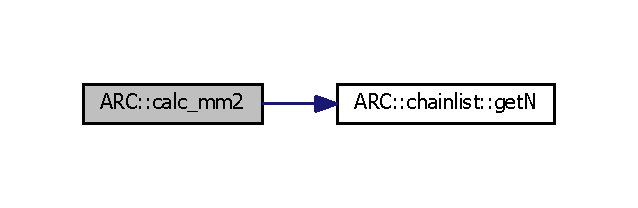
\includegraphics[width=306pt]{namespaceARC_a8d6c876e9d20067d0e8a5c1c4c2c4be6_cgraph}
\end{center}
\end{figure}
\hypertarget{namespaceARC_a70d2d18fc72d05606cb2c991ada4c64b}{}\label{namespaceARC_a70d2d18fc72d05606cb2c991ada4c64b} 
\index{A\+RC@{A\+RC}!Newtonian\+\_\+\+Ap@{Newtonian\+\_\+\+Ap}}
\index{Newtonian\+\_\+\+Ap@{Newtonian\+\_\+\+Ap}!A\+RC@{A\+RC}}
\subsubsection{\texorpdfstring{Newtonian\+\_\+\+Ap()}{Newtonian\_Ap()}}
{\footnotesize\ttfamily void A\+R\+C\+::\+Newtonian\+\_\+\+Ap (\begin{DoxyParamCaption}\item[{double}]{Aij\mbox{[}3\mbox{]},  }\item[{double \&}]{Pij,  }\item[{const double}]{xi\mbox{[}3\mbox{]},  }\item[{const double}]{xp\mbox{[}3\mbox{]},  }\item[{const double \&}]{mi,  }\item[{const double \&}]{mp,  }\item[{const double $\ast$}]{smpars }\end{DoxyParamCaption})}



Newtonian acceleration from particle p to particle i (function type of \hyperlink{namespaceARC_aed8f19a0c6ae7dc0bb3696b337d7b9f6}{A\+R\+C\+::pair\+\_\+\+Ap}) 


\begin{DoxyParams}[1]{Parameters}
\mbox{\tt out}  & {\em Aij} & acceleration vector. $Aij[1:3] = m_i m_p (xp[1:3]-xi[1:3]) / |xp-xi|^3 $. \\
\hline
\mbox{\tt out}  & {\em Pij} & potential. $ Pij = - m_i m_p /|xp-xi|^3$ \\
\hline
\mbox{\tt in}  & {\em xi} & position vector i. \\
\hline
\mbox{\tt in}  & {\em xp} & position vector p. \\
\hline
\mbox{\tt in}  & {\em mi} & particle mass i. \\
\hline
\mbox{\tt in}  & {\em mp} & particle mass p. \\
\hline
\mbox{\tt in}  & {\em smpars} & force calculation parameters (not used) \\
\hline
\end{DoxyParams}
Here is the caller graph for this function\+:
\nopagebreak
\begin{figure}[H]
\begin{center}
\leavevmode
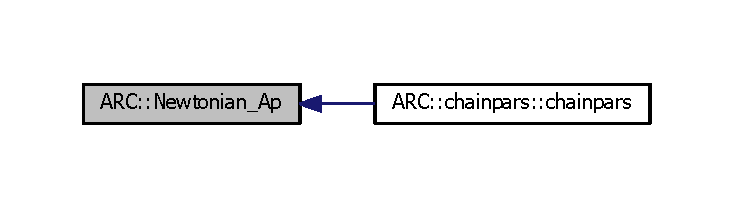
\includegraphics[width=350pt]{namespaceARC_a70d2d18fc72d05606cb2c991ada4c64b_icgraph}
\end{center}
\end{figure}
\hypertarget{namespaceARC_ab9fc6518902e918927d8c6bd3d51401d}{}\label{namespaceARC_ab9fc6518902e918927d8c6bd3d51401d} 
\index{A\+RC@{A\+RC}!Newtonian\+\_\+\+AW@{Newtonian\+\_\+\+AW}}
\index{Newtonian\+\_\+\+AW@{Newtonian\+\_\+\+AW}!A\+RC@{A\+RC}}
\subsubsection{\texorpdfstring{Newtonian\+\_\+\+A\+W()}{Newtonian\_AW()}}
{\footnotesize\ttfamily void A\+R\+C\+::\+Newtonian\+\_\+\+AW (\begin{DoxyParamCaption}\item[{double}]{Aij\mbox{[}3\mbox{]},  }\item[{double \&}]{Pij,  }\item[{double}]{p\+Wij\mbox{[}3\mbox{]},  }\item[{double \&}]{Wij,  }\item[{const double}]{xij\mbox{[}3\mbox{]},  }\item[{const double \&}]{mi,  }\item[{const double \&}]{mj,  }\item[{const double $\ast$}]{smpars }\end{DoxyParamCaption})}



Newtonian acceleration and $\partial W_{ij}/\partial \mathbf{x}_i$ from particle j to particle i (function type of \hyperlink{namespaceARC_a5c4308ca4a8d0e0ff59fdce30f00274c}{A\+R\+C\+::pair\+\_\+\+AW}) 


\begin{DoxyParams}[1]{Parameters}
\mbox{\tt out}  & {\em Aij} & Newtonian acceleration vector for i particle from particle j. $Aij[1:3] = m_i m_j xij[1:3] / |xij|^3 $. \\
\hline
\mbox{\tt out}  & {\em Pij} & Newtonian potential of i from j. $ Pij = -m_i m_j /|xij| $ \\
\hline
\mbox{\tt out}  & {\em p\+Wij} & T\+TL time transformation function partial derivates (component from j to i) $\partial W_{ij}/\partial \mathbf{x}_i$ (used for T\+TL method). $pWij[1:3] = mm_{ij} xij[1:3] /|xij|^3 $. (Total value is $\frac{\partial W}{\partial \mathbf{x}_i} = \sum_{j} mm_{ij} \mathbf{x}_{ij}/|\mathbf{x}_{ij}|^3$) \\
\hline
\mbox{\tt out}  & {\em Wij} & T\+TL time transformation function component with i,j (used for T\+TL method) $Wij = mm_{ij} /|xij|^3$ total value is $ W = \sum_{i<j} mm_{ij} /|xij| $ \\
\hline
\mbox{\tt in}  & {\em xij} & relative position vector \mbox{[}1\+:3\mbox{]} $ \mathbf{x_j} - \mathbf{x_i} $ \\
\hline
\mbox{\tt in}  & {\em mi} & particle i mass. \\
\hline
\mbox{\tt in}  & {\em mj} & particle j mass. \\
\hline
\mbox{\tt in}  & {\em smpars} & array of double\mbox{[}2\mbox{]}.
\begin{DoxyItemize}
\item First element is smooth mass coefficient mm2 $ \sum_{i<j} m_i m_j /(N(N-1)/2) $ (can be calculated by \hyperlink{namespaceARC_a8d6c876e9d20067d0e8a5c1c4c2c4be6}{calc\+\_\+mm2()}); ~\newline

\item Second element is adiustable parameter epi. 1) If epi$>$0\+: if $m_i m_j < epi mm2$\+: $ mm_{ij} = mm2$ else\+: $ mm_ij = 0$ 2) If epi$<$0\+: $mm_{ij} = m_i m_j$.~\newline

\end{DoxyItemize}\\
\hline
\end{DoxyParams}
Here is the caller graph for this function\+:
\nopagebreak
\begin{figure}[H]
\begin{center}
\leavevmode
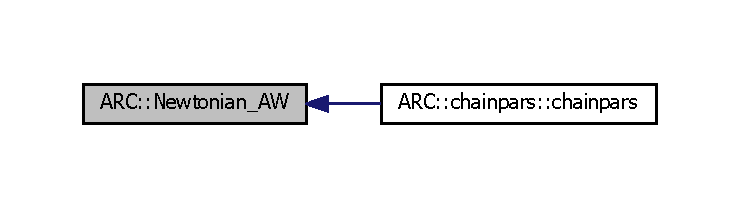
\includegraphics[width=350pt]{namespaceARC_ab9fc6518902e918927d8c6bd3d51401d_icgraph}
\end{center}
\end{figure}

\hypertarget{namespaceEP}{}\section{EP Namespace Reference}
\label{namespaceEP}\index{EP@{EP}}


For extrapolation related functions.  


\subsection*{Functions}
\begin{DoxyCompactItemize}
\item 
void \hyperlink{namespaceEP_a6197a74bc7ca232ffcc84872d8f4f779}{seq\+\_\+\+Harmonic} (int step\mbox{[}$\,$\mbox{]}, const std\+::size\+\_\+t itermax)
\begin{DoxyCompactList}\small\item\em Generate Harmonic sequence \{h, h/2, h/3, h/4 ...\}. \end{DoxyCompactList}\item 
void \hyperlink{namespaceEP_afaef3617ed3fb4ad4627c19e955c5457}{seq\+\_\+\+Romberg} (int step\mbox{[}$\,$\mbox{]}, const std\+::size\+\_\+t itermax)
\begin{DoxyCompactList}\small\item\em Generate Romberg (even) sequence \{h, h/2, h/4, h/8 ...\}. \end{DoxyCompactList}\item 
void \hyperlink{namespaceEP_a1c85d6f300251929ac82736e54760652}{seq\+\_\+\+BS} (int step\mbox{[}$\,$\mbox{]}, const std\+::size\+\_\+t itermax)
\begin{DoxyCompactList}\small\item\em Generate Bulirsch \& Stoer sequence \{h, h/2, h/3, h/4, h/6, h/8 ...\}. \end{DoxyCompactList}\item 
void \hyperlink{namespaceEP_a691e74f494e1137b68389a2bd93f92c0}{seq\+\_\+\+Hairer} (int step\mbox{[}$\,$\mbox{]}, const std\+::size\+\_\+t itermax)
\begin{DoxyCompactList}\small\item\em Generate E. Hairer (4k) sequences \{h/2, h/6, h/10, h/14 ...\}. \end{DoxyCompactList}\item 
double \hyperlink{namespaceEP_a8f951202841accc906325f37f9e592af}{polynomial\+\_\+recursive\+\_\+formula} (const double ti1k1, const double tik1, const double hr)
\begin{DoxyCompactList}\small\item\em Polynomial\+\_\+recursion\+\_\+formula. \end{DoxyCompactList}\item 
double \hyperlink{namespaceEP_afe6d08bb36343e39ebbbd4406dc9989f}{rational\+\_\+recursive\+\_\+formula} (const double ti1k2, const double ti1k1, const double tik1, const double hr)
\begin{DoxyCompactList}\small\item\em Rational\+\_\+recursion formula. \end{DoxyCompactList}\item 
void \hyperlink{namespaceEP_ae89d6690a891336eef708e90e575a2be}{polynomial\+\_\+extrapolation} (double $\ast$$\ast$Tn, double $\ast$Tnew, const int step\mbox{[}$\,$\mbox{]}, const std\+::size\+\_\+t Tsize, const std\+::size\+\_\+t n)
\begin{DoxyCompactList}\small\item\em Polynomial extrapolation of Tsize number of data together. \end{DoxyCompactList}\item 
void \hyperlink{namespaceEP_a069470acd4f6c52b2ebb68afcf4528ab}{rational\+\_\+extrapolation} (double $\ast$$\ast$Tn, double $\ast$Tnew, const int step\mbox{[}$\,$\mbox{]}, const std\+::size\+\_\+t Tsize, const std\+::size\+\_\+t n)
\begin{DoxyCompactList}\small\item\em Rational extrapolation of Tsize number of data together. \end{DoxyCompactList}\item 
double \hyperlink{namespaceEP_ab0499a8ae6cab209fc0cca6a47b166f3}{extrapolation\+\_\+error} (double $\ast$$\ast$Tn, const std\+::size\+\_\+t Tsize, const std\+::size\+\_\+t n)
\begin{DoxyCompactList}\small\item\em Error estimation. \end{DoxyCompactList}\item 
double \hyperlink{namespaceEP_a6d54b765511d661bb4267799ff1a804f}{H\+\_\+opt\+\_\+factor} (const double err, const double exp, const int n)
\begin{DoxyCompactList}\small\item\em Next step optimized factor estimation (based on the extrapolation order n) \end{DoxyCompactList}\item 
void \hyperlink{namespaceEP_a92c709f3757c872402d2fcf954c3e2de}{binomial\+\_\+recursive\+\_\+generator} (int $\ast$bn, const int $\ast$bp, const std\+::size\+\_\+t n)
\begin{DoxyCompactList}\small\item\em Binomial coefficients generator. \end{DoxyCompactList}\item 
void \hyperlink{namespaceEP_ad1bbde38ef63ce2a0672843d598770b8}{Hermite\+\_\+interpolation\+\_\+coefficients} (double $\ast$$\ast$coff, const double $\ast$x, double $\ast$$\ast$f, double $\ast$$\ast$$\ast$df, const int ndata, const int npoints, const int $\ast$nlev)
\begin{DoxyCompactList}\small\item\em Hermite interpolation coefficients. \end{DoxyCompactList}\item 
void \hyperlink{namespaceEP_a10270a1ba230322545fff5bc06d94659}{Hermite\+\_\+interpolation\+\_\+polynomial} (double xn, double $\ast$fxn, double $\ast$$\ast$coff, const double $\ast$x, const int ndata, const int npoints, const int $\ast$nlev)
\begin{DoxyCompactList}\small\item\em Hermite interpolation polynomial. \end{DoxyCompactList}\end{DoxyCompactItemize}


\subsection{Detailed Description}
For extrapolation related functions. 

\subsection{Function Documentation}
\hypertarget{namespaceEP_a92c709f3757c872402d2fcf954c3e2de}{}\label{namespaceEP_a92c709f3757c872402d2fcf954c3e2de} 
\index{EP@{EP}!binomial\+\_\+recursive\+\_\+generator@{binomial\+\_\+recursive\+\_\+generator}}
\index{binomial\+\_\+recursive\+\_\+generator@{binomial\+\_\+recursive\+\_\+generator}!EP@{EP}}
\subsubsection{\texorpdfstring{binomial\+\_\+recursive\+\_\+generator()}{binomial\_recursive\_generator()}}
{\footnotesize\ttfamily void E\+P\+::binomial\+\_\+recursive\+\_\+generator (\begin{DoxyParamCaption}\item[{int $\ast$}]{bn,  }\item[{const int $\ast$}]{bp,  }\item[{const std\+::size\+\_\+t}]{n }\end{DoxyParamCaption})}



Binomial coefficients generator. 

Generate the next binomial sequence (n 1\+:n) based on (n-\/1 1\+:n-\/1) 
\begin{DoxyParams}[1]{Parameters}
\mbox{\tt in}  & {\em bp} & n-\/1 sequence array (size of n-\/1) \\
\hline
\mbox{\tt in}  & {\em bn} & new sequence array (size of n) \\
\hline
\mbox{\tt in}  & {\em n} & new sequence index \\
\hline
\end{DoxyParams}
\hypertarget{namespaceEP_ab0499a8ae6cab209fc0cca6a47b166f3}{}\label{namespaceEP_ab0499a8ae6cab209fc0cca6a47b166f3} 
\index{EP@{EP}!extrapolation\+\_\+error@{extrapolation\+\_\+error}}
\index{extrapolation\+\_\+error@{extrapolation\+\_\+error}!EP@{EP}}
\subsubsection{\texorpdfstring{extrapolation\+\_\+error()}{extrapolation\_error()}}
{\footnotesize\ttfamily double E\+P\+::extrapolation\+\_\+error (\begin{DoxyParamCaption}\item[{double $\ast$$\ast$}]{Tn,  }\item[{const std\+::size\+\_\+t}]{Tsize,  }\item[{const std\+::size\+\_\+t}]{n }\end{DoxyParamCaption})}



Error estimation. 

Error calculation based on $ T_{n,n} $ and $ T_{n,n-1} $ Calculate the value of $ 2 \frac{T_{n,n} - T_{n,n-1}}{\sqrt{T_{n,n}^2 + T_{n,n-1}^2}} $ via looping all Tsize data and select the maximum value as error 
\begin{DoxyParams}[1]{Parameters}
\mbox{\tt in}  & {\em Tn} & $ T_{n,(1..n)} $ array (two dimensional array with size \mbox{[}n\mbox{]}\mbox{[}Tsize\mbox{]}, where first \mbox{[}\mbox{]} indicate the extrapolation order and second \mbox{[}\mbox{]} indicate individual data \\
\hline
\mbox{\tt in}  & {\em Tsize} & data array size \\
\hline
\mbox{\tt in}  & {\em n} & iteration step index (count from 0) \\
\hline
\end{DoxyParams}
\begin{DoxyReturn}{Returns}
maximum error 
\end{DoxyReturn}
\hypertarget{namespaceEP_a6d54b765511d661bb4267799ff1a804f}{}\label{namespaceEP_a6d54b765511d661bb4267799ff1a804f} 
\index{EP@{EP}!H\+\_\+opt\+\_\+factor@{H\+\_\+opt\+\_\+factor}}
\index{H\+\_\+opt\+\_\+factor@{H\+\_\+opt\+\_\+factor}!EP@{EP}}
\subsubsection{\texorpdfstring{H\+\_\+opt\+\_\+factor()}{H\_opt\_factor()}}
{\footnotesize\ttfamily double E\+P\+::\+H\+\_\+opt\+\_\+factor (\begin{DoxyParamCaption}\item[{const double}]{err,  }\item[{const double}]{exp,  }\item[{const int}]{n }\end{DoxyParamCaption})}



Next step optimized factor estimation (based on the extrapolation order n) 

Calculate the modification factor for next extrapolation intergration step (assume next maximum extrapolation order is n). ~\newline
(new step size) Hnew $\sim$ (old step size) H $\ast$ ({\itshape exp/{\itshape err})$\ast$$\ast$1/}(2n+3) 
\begin{DoxyParams}[1]{Parameters}
\mbox{\tt in}  & {\em err} & error of current extrapolation from $ T_{n,n-1} $ to $ T_{n,n} $ \\
\hline
\mbox{\tt in}  & {\em exp} & expected error \\
\hline
\mbox{\tt in}  & {\em n} & current sub-\/step number return\+: optimized factor (H = H$\ast$factor) \\
\hline
\end{DoxyParams}
\hypertarget{namespaceEP_ad1bbde38ef63ce2a0672843d598770b8}{}\label{namespaceEP_ad1bbde38ef63ce2a0672843d598770b8} 
\index{EP@{EP}!Hermite\+\_\+interpolation\+\_\+coefficients@{Hermite\+\_\+interpolation\+\_\+coefficients}}
\index{Hermite\+\_\+interpolation\+\_\+coefficients@{Hermite\+\_\+interpolation\+\_\+coefficients}!EP@{EP}}
\subsubsection{\texorpdfstring{Hermite\+\_\+interpolation\+\_\+coefficients()}{Hermite\_interpolation\_coefficients()}}
{\footnotesize\ttfamily void E\+P\+::\+Hermite\+\_\+interpolation\+\_\+coefficients (\begin{DoxyParamCaption}\item[{double $\ast$$\ast$}]{coff,  }\item[{const double $\ast$}]{x,  }\item[{double $\ast$$\ast$}]{f,  }\item[{double $\ast$$\ast$$\ast$}]{df,  }\item[{const int}]{ndata,  }\item[{const int}]{npoints,  }\item[{const int $\ast$}]{nlev }\end{DoxyParamCaption})}



Hermite interpolation coefficients. 

Generate Hermite interpolation polynomial coefficients (see example in \href{https://en.wikipedia.org/wiki/Hermite_interpolation}{\tt https\+://en.\+wikipedia.\+org/wiki/\+Hermite\+\_\+interpolation}) 
\begin{DoxyParams}[1]{Parameters}
\mbox{\tt out}  & {\em coff} & two dimensional array storing the interpolation coefficients \mbox{[}ndata\mbox{]}\mbox{[} $\sum_j nlev_j$\mbox{]} \\
\hline
\mbox{\tt in}  & {\em x} & one dimensional array that store the positions \mbox{[}npoints\mbox{]} \\
\hline
\mbox{\tt in}  & {\em f} & two dimensional array that store the f(x) \mbox{[}npoints\mbox{]}\mbox{[}ndata\mbox{]} \\
\hline
\mbox{\tt in}  & {\em df} & three dimensional array that store the f$^\wedge$(k)(x) \mbox{[}k\mbox{]}\mbox{[}npoints\mbox{]}\mbox{[}ndata\mbox{]} \\
\hline
\mbox{\tt in}  & {\em ndata} & number of different type of data for interpolation \\
\hline
\mbox{\tt in}  & {\em npoints} & number of position points. \\
\hline
\mbox{\tt in}  & {\em nlev} & one dimensional array that store the maximum difference level for each position (f$^\wedge$(0)(x) count as 1) \\
\hline
\end{DoxyParams}
\hypertarget{namespaceEP_a10270a1ba230322545fff5bc06d94659}{}\label{namespaceEP_a10270a1ba230322545fff5bc06d94659} 
\index{EP@{EP}!Hermite\+\_\+interpolation\+\_\+polynomial@{Hermite\+\_\+interpolation\+\_\+polynomial}}
\index{Hermite\+\_\+interpolation\+\_\+polynomial@{Hermite\+\_\+interpolation\+\_\+polynomial}!EP@{EP}}
\subsubsection{\texorpdfstring{Hermite\+\_\+interpolation\+\_\+polynomial()}{Hermite\_interpolation\_polynomial()}}
{\footnotesize\ttfamily void E\+P\+::\+Hermite\+\_\+interpolation\+\_\+polynomial (\begin{DoxyParamCaption}\item[{double}]{xn,  }\item[{double $\ast$}]{fxn,  }\item[{double $\ast$$\ast$}]{coff,  }\item[{const double $\ast$}]{x,  }\item[{const int}]{ndata,  }\item[{const int}]{npoints,  }\item[{const int $\ast$}]{nlev }\end{DoxyParamCaption})}



Hermite interpolation polynomial. 

Return the interpolation result based on polynomial coefficients generated from \hyperlink{namespaceEP_ad1bbde38ef63ce2a0672843d598770b8}{E\+P\+::\+Hermite\+\_\+interpolation\+\_\+coefficients()} 
\begin{DoxyParams}[1]{Parameters}
\mbox{\tt in}  & {\em xn} & position want to get interpolation value \\
\hline
\mbox{\tt out}  & {\em fxn} & one dimensional array that store the interpolation results \mbox{[}ndata\mbox{]} \\
\hline
\mbox{\tt in}  & {\em coff} & two dimensional array storing the interpolation coefficients \mbox{[}ndata\mbox{]}\mbox{[} $\sum_j nlev_j$\mbox{]} \\
\hline
\mbox{\tt in}  & {\em x} & one dimensional array that store the known positions \mbox{[}npoints\mbox{]}. \\
\hline
\mbox{\tt in}  & {\em ndata} & number of different type of data for interpolation \\
\hline
\mbox{\tt in}  & {\em npoints} & number of position points. \\
\hline
\mbox{\tt in}  & {\em nlev} & one dimensional array that store the maximum difference level for each position (f$^\wedge$(0)(x) count as 1) \\
\hline
\end{DoxyParams}
\hypertarget{namespaceEP_ae89d6690a891336eef708e90e575a2be}{}\label{namespaceEP_ae89d6690a891336eef708e90e575a2be} 
\index{EP@{EP}!polynomial\+\_\+extrapolation@{polynomial\+\_\+extrapolation}}
\index{polynomial\+\_\+extrapolation@{polynomial\+\_\+extrapolation}!EP@{EP}}
\subsubsection{\texorpdfstring{polynomial\+\_\+extrapolation()}{polynomial\_extrapolation()}}
{\footnotesize\ttfamily void E\+P\+::polynomial\+\_\+extrapolation (\begin{DoxyParamCaption}\item[{double $\ast$$\ast$}]{Tn,  }\item[{double $\ast$}]{Tnew,  }\item[{const int}]{step\mbox{[}$\,$\mbox{]},  }\item[{const std\+::size\+\_\+t}]{Tsize,  }\item[{const std\+::size\+\_\+t}]{n }\end{DoxyParamCaption})}



Polynomial extrapolation of Tsize number of data together. 

Iterate $ T_{n,(1..n)} $ based on $ T_{n-1,(1...n-1)} $ and $ T_{n,1} $ Notice the Tsize number of data in {\itshape Tn} and {\itshape Tnew} are independent data that need to be extrapolated individually (each data is an individual $ T_{x,x} $) 
\begin{DoxyParams}[1]{Parameters}
\mbox{\tt in,out}  & {\em Tn} & two dimensional array of $ T_{n-1,(1...n-1)} $ (size of \mbox{[}n+1\mbox{]}\mbox{[}Tsize\mbox{]}; first \mbox{[}\mbox{]} indicate the extrapolation order (1...n), second \mbox{[}\mbox{]} indicate the different data), will be updated to $ T_{n,(1..n)} $ \\
\hline
\mbox{\tt in,out}  & {\em Tnew} & one dimensional array of $ T_{n,1} $ (size of Tsize with different data), will be updated to $ T_n $ \\
\hline
\mbox{\tt in}  & {\em step} & step sequence (from sequence generators) \\
\hline
\mbox{\tt in}  & {\em Tsize} & data array size \\
\hline
\mbox{\tt in}  & {\em n} & the new iteration step index in {\itshape step} (count from 0) \\
\hline
\end{DoxyParams}
\hypertarget{namespaceEP_a8f951202841accc906325f37f9e592af}{}\label{namespaceEP_a8f951202841accc906325f37f9e592af} 
\index{EP@{EP}!polynomial\+\_\+recursive\+\_\+formula@{polynomial\+\_\+recursive\+\_\+formula}}
\index{polynomial\+\_\+recursive\+\_\+formula@{polynomial\+\_\+recursive\+\_\+formula}!EP@{EP}}
\subsubsection{\texorpdfstring{polynomial\+\_\+recursive\+\_\+formula()}{polynomial\_recursive\_formula()}}
{\footnotesize\ttfamily double E\+P\+::polynomial\+\_\+recursive\+\_\+formula (\begin{DoxyParamCaption}\item[{const double}]{ti1k1,  }\item[{const double}]{tik1,  }\item[{const double}]{hr }\end{DoxyParamCaption})}



Polynomial\+\_\+recursion\+\_\+formula. 

Using Polynomial function\+: $ T_{i,k} = T_{i,k-1} + \frac{T_{i,k-1} - T_{i-1,k-1}}{(h_{i-k}/h_i)^2 -1} $ ~\newline

\begin{DoxyParams}[1]{Parameters}
\mbox{\tt in}  & {\em ti1k1} & $ t_{i-1,k-1} $ \\
\hline
\mbox{\tt in}  & {\em tik1} & $ t_{i,k-1} $ \\
\hline
\mbox{\tt in}  & {\em hr} & $ h_{i-k/h_i} $ \\
\hline
\end{DoxyParams}
\begin{DoxyReturn}{Returns}
$ T_{i,k} $ 
\end{DoxyReturn}
\hypertarget{namespaceEP_a069470acd4f6c52b2ebb68afcf4528ab}{}\label{namespaceEP_a069470acd4f6c52b2ebb68afcf4528ab} 
\index{EP@{EP}!rational\+\_\+extrapolation@{rational\+\_\+extrapolation}}
\index{rational\+\_\+extrapolation@{rational\+\_\+extrapolation}!EP@{EP}}
\subsubsection{\texorpdfstring{rational\+\_\+extrapolation()}{rational\_extrapolation()}}
{\footnotesize\ttfamily void E\+P\+::rational\+\_\+extrapolation (\begin{DoxyParamCaption}\item[{double $\ast$$\ast$}]{Tn,  }\item[{double $\ast$}]{Tnew,  }\item[{const int}]{step\mbox{[}$\,$\mbox{]},  }\item[{const std\+::size\+\_\+t}]{Tsize,  }\item[{const std\+::size\+\_\+t}]{n }\end{DoxyParamCaption})}



Rational extrapolation of Tsize number of data together. 

Iterate $ T_{n,(1..n)} $ based on $ T_{n-1,(1...n-1)} $ and $ T_{n,1} $ ~\newline
Notice the Tsize number of data in {\itshape Tn} and {\itshape Tnew} are independent data that need to be extrapolated individually (each data is an individual $ T_{x,x} $) 
\begin{DoxyParams}[1]{Parameters}
\mbox{\tt in,out}  & {\em Tn} & two dimensial array of $ T_{n-1,(1...n-1)} $ (size of \mbox{[}n+1\mbox{]}\mbox{[}Tsize\mbox{]}; first \mbox{[}\mbox{]} indicate the extrapolation order (1...n), second \mbox{[}\mbox{]} indicate the different data) will be updated to $ T_{n,(1..n)} $ \\
\hline
\mbox{\tt in,out}  & {\em Tnew} & one dimensional array of $ T_{n,1} $ (size of Tsize with different data), will be updated to $ T_n $ \\
\hline
\mbox{\tt in}  & {\em step} & step sequence (from sequence generators) \\
\hline
\mbox{\tt in}  & {\em Tsize} & data array size \\
\hline
\mbox{\tt in}  & {\em n} & the new iteration step index in {\itshape step} (count from 0) \\
\hline
\end{DoxyParams}
\hypertarget{namespaceEP_afe6d08bb36343e39ebbbd4406dc9989f}{}\label{namespaceEP_afe6d08bb36343e39ebbbd4406dc9989f} 
\index{EP@{EP}!rational\+\_\+recursive\+\_\+formula@{rational\+\_\+recursive\+\_\+formula}}
\index{rational\+\_\+recursive\+\_\+formula@{rational\+\_\+recursive\+\_\+formula}!EP@{EP}}
\subsubsection{\texorpdfstring{rational\+\_\+recursive\+\_\+formula()}{rational\_recursive\_formula()}}
{\footnotesize\ttfamily double E\+P\+::rational\+\_\+recursive\+\_\+formula (\begin{DoxyParamCaption}\item[{const double}]{ti1k2,  }\item[{const double}]{ti1k1,  }\item[{const double}]{tik1,  }\item[{const double}]{hr }\end{DoxyParamCaption})}



Rational\+\_\+recursion formula. 

Using rational function\+: $ T_{i,k} = T_{i,k-1} + \frac{ T_{i,k-1} - T_{i-1,k-1} }{ \left( \frac{ h_{i-k} }{ h_i } \right)^2 \left( 1- \frac{ T_{i,k-1} - T_{i-1,k-1} }{ T_{i,k-1} - T_{i-1,k-2} } \right) -1} $ 
\begin{DoxyParams}[1]{Parameters}
\mbox{\tt in}  & {\em ti1k2} & $ T_{i-1,k-2} $ \\
\hline
\mbox{\tt in}  & {\em ti1k1} & $ T_{i-1,k-1} $ \\
\hline
\mbox{\tt in}  & {\em tik1} & $ T_{i,k-1} $ \\
\hline
\mbox{\tt in}  & {\em hr} & $ h_{i-k/h_i} $ \\
\hline
\end{DoxyParams}
\begin{DoxyReturn}{Returns}
$ T_{i,k} $ 
\end{DoxyReturn}
\hypertarget{namespaceEP_a1c85d6f300251929ac82736e54760652}{}\label{namespaceEP_a1c85d6f300251929ac82736e54760652} 
\index{EP@{EP}!seq\+\_\+\+BS@{seq\+\_\+\+BS}}
\index{seq\+\_\+\+BS@{seq\+\_\+\+BS}!EP@{EP}}
\subsubsection{\texorpdfstring{seq\+\_\+\+B\+S()}{seq\_BS()}}
{\footnotesize\ttfamily void E\+P\+::seq\+\_\+\+BS (\begin{DoxyParamCaption}\item[{int}]{step\mbox{[}$\,$\mbox{]},  }\item[{const std\+::size\+\_\+t}]{itermax }\end{DoxyParamCaption})}



Generate Bulirsch \& Stoer sequence \{h, h/2, h/3, h/4, h/6, h/8 ...\}. 


\begin{DoxyParams}[1]{Parameters}
\mbox{\tt out}  & {\em step} & sequence array for storing the division steps \{1, 2, 3, 4, 6 ...\} \\
\hline
\mbox{\tt in}  & {\em itermax} & array size \\
\hline
\end{DoxyParams}
\hypertarget{namespaceEP_a691e74f494e1137b68389a2bd93f92c0}{}\label{namespaceEP_a691e74f494e1137b68389a2bd93f92c0} 
\index{EP@{EP}!seq\+\_\+\+Hairer@{seq\+\_\+\+Hairer}}
\index{seq\+\_\+\+Hairer@{seq\+\_\+\+Hairer}!EP@{EP}}
\subsubsection{\texorpdfstring{seq\+\_\+\+Hairer()}{seq\_Hairer()}}
{\footnotesize\ttfamily void E\+P\+::seq\+\_\+\+Hairer (\begin{DoxyParamCaption}\item[{int}]{step\mbox{[}$\,$\mbox{]},  }\item[{const std\+::size\+\_\+t}]{itermax }\end{DoxyParamCaption})}



Generate E. Hairer (4k) sequences \{h/2, h/6, h/10, h/14 ...\}. 


\begin{DoxyParams}[1]{Parameters}
\mbox{\tt out}  & {\em step} & sequence array for storing the division steps \{2, 6, 10, 14 ...\} \\
\hline
\mbox{\tt in}  & {\em itermax} & array size \\
\hline
\end{DoxyParams}
\hypertarget{namespaceEP_a6197a74bc7ca232ffcc84872d8f4f779}{}\label{namespaceEP_a6197a74bc7ca232ffcc84872d8f4f779} 
\index{EP@{EP}!seq\+\_\+\+Harmonic@{seq\+\_\+\+Harmonic}}
\index{seq\+\_\+\+Harmonic@{seq\+\_\+\+Harmonic}!EP@{EP}}
\subsubsection{\texorpdfstring{seq\+\_\+\+Harmonic()}{seq\_Harmonic()}}
{\footnotesize\ttfamily void E\+P\+::seq\+\_\+\+Harmonic (\begin{DoxyParamCaption}\item[{int}]{step\mbox{[}$\,$\mbox{]},  }\item[{const std\+::size\+\_\+t}]{itermax }\end{DoxyParamCaption})}



Generate Harmonic sequence \{h, h/2, h/3, h/4 ...\}. 


\begin{DoxyParams}[1]{Parameters}
\mbox{\tt out}  & {\em step} & sequence array for storing the division steps \{1, 2, 3, 4 ...\} \\
\hline
\mbox{\tt in}  & {\em itermax} & array size \\
\hline
\end{DoxyParams}
\hypertarget{namespaceEP_afaef3617ed3fb4ad4627c19e955c5457}{}\label{namespaceEP_afaef3617ed3fb4ad4627c19e955c5457} 
\index{EP@{EP}!seq\+\_\+\+Romberg@{seq\+\_\+\+Romberg}}
\index{seq\+\_\+\+Romberg@{seq\+\_\+\+Romberg}!EP@{EP}}
\subsubsection{\texorpdfstring{seq\+\_\+\+Romberg()}{seq\_Romberg()}}
{\footnotesize\ttfamily void E\+P\+::seq\+\_\+\+Romberg (\begin{DoxyParamCaption}\item[{int}]{step\mbox{[}$\,$\mbox{]},  }\item[{const std\+::size\+\_\+t}]{itermax }\end{DoxyParamCaption})}



Generate Romberg (even) sequence \{h, h/2, h/4, h/8 ...\}. 


\begin{DoxyParams}[1]{Parameters}
\mbox{\tt out}  & {\em step} & sequence array for storing the division steps \{1, 2, 4, 8 ...\} \\
\hline
\mbox{\tt in}  & {\em itermax} & array size \\
\hline
\end{DoxyParams}

\hypertarget{namespaceNTA}{}\section{N\+TA Namespace Reference}
\label{namespaceNTA}\index{N\+TA@{N\+TA}}


Namespace for Newtonian Interaction related functions.  


\subsection*{Classes}
\begin{DoxyCompactItemize}
\item 
class \hyperlink{classNTA_1_1Newtonian__pars}{Newtonian\+\_\+pars}
\begin{DoxyCompactList}\small\item\em Newtonian Interaction and time transformation function parameter class. \end{DoxyCompactList}\end{DoxyCompactItemize}
\subsection*{Typedefs}
\begin{DoxyCompactItemize}
\item 
typedef double \hyperlink{namespaceNTA_a19ccaac066849b26305dbbbee129fa0e}{double3}\mbox{[}3\mbox{]}
\end{DoxyCompactItemize}
\subsection*{Functions}
\begin{DoxyCompactItemize}
\item 
int \hyperlink{namespaceNTA_aad37ae368f0a920088e180a73187685a}{Newtonian\+\_\+\+AW} (double Aij\mbox{[}3\mbox{]}, double \&Pij, double p\+Wij\mbox{[}3\mbox{]}, double \&Wij, const double xij\mbox{[}3\mbox{]}, const \hyperlink{classParticle}{Particle} \&pi, const \hyperlink{classParticle}{Particle} \&pj, \hyperlink{classNTA_1_1Newtonian__pars}{Newtonian\+\_\+pars} $\ast$pars)
\begin{DoxyCompactList}\small\item\em Newtonian acceleration and $\partial W_{ij}/\partial \mathbf{x}_i$ from particle j to particle i (function type of \hyperlink{namespaceARC_a270b4c77765cacf073a5ef5f928f1d63}{A\+R\+C\+::pair\+\_\+\+AW}) \end{DoxyCompactList}\item 
void \hyperlink{namespaceNTA_a5b1a4fcaa09041cdf89a6b3122815c56}{Newtonian\+\_\+ext\+Acc} (\hyperlink{namespaceNTA_a19ccaac066849b26305dbbbee129fa0e}{double3} $\ast$acc, const double t, \hyperlink{classParticle}{Particle} $\ast$p, const int np, \hyperlink{classParticle}{Particle} $\ast$pert, \hyperlink{namespaceNTA_a19ccaac066849b26305dbbbee129fa0e}{double3} $\ast$pertf, const int npert, \hyperlink{classNTA_1_1Newtonian__pars}{Newtonian\+\_\+pars} $\ast$pars)
\begin{DoxyCompactList}\small\item\em Newtonian acceleration from perturber pert to particle p (function type of \hyperlink{namespaceARC_a7aeda3b3bd009af7ac964748834dd312}{A\+R\+C\+::ext\+\_\+\+Acc}) \end{DoxyCompactList}\item 
double \hyperlink{namespaceNTA_a5125fd91a773d67901c4e0f8896e3dca}{Newtonian\+\_\+kepler\+\_\+period} (const double m1, const double m2, const double dx\mbox{[}3\mbox{]}, const double dv\mbox{[}3\mbox{]}, \hyperlink{classNTA_1_1Newtonian__pars}{Newtonian\+\_\+pars} $\ast$pars)
\begin{DoxyCompactList}\small\item\em Newtonian two-\/body kepler period. \end{DoxyCompactList}\item 
void \hyperlink{namespaceNTA_a02d22f02e21004b264c8257a5ffbb600}{calc\+\_\+kepler\+\_\+orbit\+\_\+par} (double \&semi, double \&peri, double \&ecc, double angle\mbox{[}3\mbox{]}, double \&true\+\_\+anomaly, double \&ecc\+\_\+anomaly, double \&mean\+\_\+anomaly, const double m, const double dx\mbox{[}3\mbox{]}, const double dv\mbox{[}3\mbox{]})
\begin{DoxyCompactList}\small\item\em Calculate parameters of two-\/body motion. \end{DoxyCompactList}\item 
void \hyperlink{namespaceNTA_a621b3643cd91a5a7ea23b7b22481f121}{kepler\+\_\+orbit\+\_\+generator} (double x1\mbox{[}3\mbox{]}, double x2\mbox{[}3\mbox{]}, double v1\mbox{[}3\mbox{]}, double v2\mbox{[}3\mbox{]}, const double m1, const double m2, const double semi, const double ecc, const double angle\mbox{[}3\mbox{]}, const double ecc\+\_\+anomaly)
\end{DoxyCompactItemize}


\subsection{Detailed Description}
Namespace for Newtonian Interaction related functions. 

In the special applications of N-\/body simulations with Newtonian gravity, the Newtonian acceleration functions should be defined. The corresponding timescale to determing the next integrating step should also be provided. This is the namespace where all these functions are provided. 

\subsection{Typedef Documentation}
\hypertarget{namespaceNTA_a19ccaac066849b26305dbbbee129fa0e}{}\label{namespaceNTA_a19ccaac066849b26305dbbbee129fa0e} 
\index{N\+TA@{N\+TA}!double3@{double3}}
\index{double3@{double3}!N\+TA@{N\+TA}}
\subsubsection{\texorpdfstring{double3}{double3}}
{\footnotesize\ttfamily typedef double N\+T\+A\+::double3\mbox{[}3\mbox{]}}



\subsection{Function Documentation}
\hypertarget{namespaceNTA_a02d22f02e21004b264c8257a5ffbb600}{}\label{namespaceNTA_a02d22f02e21004b264c8257a5ffbb600} 
\index{N\+TA@{N\+TA}!calc\+\_\+kepler\+\_\+orbit\+\_\+par@{calc\+\_\+kepler\+\_\+orbit\+\_\+par}}
\index{calc\+\_\+kepler\+\_\+orbit\+\_\+par@{calc\+\_\+kepler\+\_\+orbit\+\_\+par}!N\+TA@{N\+TA}}
\subsubsection{\texorpdfstring{calc\+\_\+kepler\+\_\+orbit\+\_\+par()}{calc\_kepler\_orbit\_par()}}
{\footnotesize\ttfamily void N\+T\+A\+::calc\+\_\+kepler\+\_\+orbit\+\_\+par (\begin{DoxyParamCaption}\item[{double \&}]{semi,  }\item[{double \&}]{peri,  }\item[{double \&}]{ecc,  }\item[{double}]{angle\mbox{[}3\mbox{]},  }\item[{double \&}]{true\+\_\+anomaly,  }\item[{double \&}]{ecc\+\_\+anomaly,  }\item[{double \&}]{mean\+\_\+anomaly,  }\item[{const double}]{m,  }\item[{const double}]{dx\mbox{[}3\mbox{]},  }\item[{const double}]{dv\mbox{[}3\mbox{]} }\end{DoxyParamCaption})}



Calculate parameters of two-\/body motion. 

Calcuate the basic parameters of two-\/body motions 
\begin{DoxyParams}[1]{Parameters}
\mbox{\tt out}  & {\em semi} & semi-\/major axis \\
\hline
\mbox{\tt out}  & {\em peri} & period \\
\hline
\mbox{\tt out}  & {\em ecc} & eccentricity \\
\hline
\mbox{\tt out}  & {\em angle} & three rotational angles\+: inclination, z-\/axis rotation, orbital-\/plane rotation \\
\hline
\mbox{\tt out}  & {\em true\+\_\+anomaly} & true anomaly \\
\hline
\mbox{\tt out}  & {\em ecc\+\_\+anomaly} & eccentricity anomaly \\
\hline
\mbox{\tt out}  & {\em mean\+\_\+anomaly} & mean anomaly \\
\hline
\mbox{\tt in}  & {\em m} & total mass of two particles \\
\hline
\mbox{\tt in}  & {\em dx} & relative position \mbox{[}3\mbox{]} \\
\hline
\mbox{\tt in}  & {\em dv} & relative velocity \mbox{[}3\mbox{]} \\
\hline
\end{DoxyParams}
\hypertarget{namespaceNTA_a621b3643cd91a5a7ea23b7b22481f121}{}\label{namespaceNTA_a621b3643cd91a5a7ea23b7b22481f121} 
\index{N\+TA@{N\+TA}!kepler\+\_\+orbit\+\_\+generator@{kepler\+\_\+orbit\+\_\+generator}}
\index{kepler\+\_\+orbit\+\_\+generator@{kepler\+\_\+orbit\+\_\+generator}!N\+TA@{N\+TA}}
\subsubsection{\texorpdfstring{kepler\+\_\+orbit\+\_\+generator()}{kepler\_orbit\_generator()}}
{\footnotesize\ttfamily void N\+T\+A\+::kepler\+\_\+orbit\+\_\+generator (\begin{DoxyParamCaption}\item[{double}]{x1\mbox{[}3\mbox{]},  }\item[{double}]{x2\mbox{[}3\mbox{]},  }\item[{double}]{v1\mbox{[}3\mbox{]},  }\item[{double}]{v2\mbox{[}3\mbox{]},  }\item[{const double}]{m1,  }\item[{const double}]{m2,  }\item[{const double}]{semi,  }\item[{const double}]{ecc,  }\item[{const double}]{angle\mbox{[}3\mbox{]},  }\item[{const double}]{ecc\+\_\+anomaly }\end{DoxyParamCaption})}

\hypertarget{namespaceNTA_aad37ae368f0a920088e180a73187685a}{}\label{namespaceNTA_aad37ae368f0a920088e180a73187685a} 
\index{N\+TA@{N\+TA}!Newtonian\+\_\+\+AW@{Newtonian\+\_\+\+AW}}
\index{Newtonian\+\_\+\+AW@{Newtonian\+\_\+\+AW}!N\+TA@{N\+TA}}
\subsubsection{\texorpdfstring{Newtonian\+\_\+\+A\+W()}{Newtonian\_AW()}}
{\footnotesize\ttfamily int N\+T\+A\+::\+Newtonian\+\_\+\+AW (\begin{DoxyParamCaption}\item[{double}]{Aij\mbox{[}3\mbox{]},  }\item[{double \&}]{Pij,  }\item[{double}]{p\+Wij\mbox{[}3\mbox{]},  }\item[{double \&}]{Wij,  }\item[{const double}]{xij\mbox{[}3\mbox{]},  }\item[{const \hyperlink{classParticle}{Particle} \&}]{pi,  }\item[{const \hyperlink{classParticle}{Particle} \&}]{pj,  }\item[{\hyperlink{classNTA_1_1Newtonian__pars}{Newtonian\+\_\+pars} $\ast$}]{pars }\end{DoxyParamCaption})}



Newtonian acceleration and $\partial W_{ij}/\partial \mathbf{x}_i$ from particle j to particle i (function type of \hyperlink{namespaceARC_a270b4c77765cacf073a5ef5f928f1d63}{A\+R\+C\+::pair\+\_\+\+AW}) 


\begin{DoxyParams}[1]{Parameters}
\mbox{\tt out}  & {\em Aij} & Newtonian acceleration vector for i particle from particle j. $Aij[1:3] = m_i m_j xij[1:3] / |xij|^3 $. \\
\hline
\mbox{\tt out}  & {\em Pij} & Newtonian potential of i from j. $ Pij = -m_i m_j /|xij| $ \\
\hline
\mbox{\tt out}  & {\em p\+Wij} & T\+TL time transformation function partial derivates (component from j to i) $\partial W_{ij}/\partial \mathbf{x}_i$ (used for T\+TL method). $pWij[1:3] = mm_{ij} xij[1:3] /|xij|^3 $. (Total value is $\frac{\partial W}{\partial \mathbf{x}_i} = \sum_{j} mm_{ij} \mathbf{x}_{ij}/|\mathbf{x}_{ij}|^3$) \\
\hline
\mbox{\tt out}  & {\em Wij} & T\+TL time transformation function component with i,j (used for T\+TL method) $Wij = mm_{ij} /|xij|^3$ total value is $ W = \sum_{i<j} mm_{ij} /|xij| $ \\
\hline
\mbox{\tt in}  & {\em xij} & relative position vector \mbox{[}1\+:3\mbox{]} $ \mathbf{x_j} - \mathbf{x_i} $ \\
\hline
\mbox{\tt in}  & {\em pi} & particle i (get mass) \\
\hline
\mbox{\tt in}  & {\em pj} & particle j (get mass) \\
\hline
\mbox{\tt in}  & {\em pars} & Newtionian\+\_\+pars type data with members\+:
\begin{DoxyItemize}
\item mm2\+: smooth mass coefficient $ \sum_{i<j} m_i m_j /(N(N-1)/2) $ (can be calculated by calc\+\_\+mm2()); ~\newline

\item epi\+: adiustable parameter. 1) If epi$>$0\+: if $m_i m_j < epi mm2$\+: $ mm_{ij} = mm2$ else\+: $ mm_ij = 0$ 2) If epi$<$0\+: $mm_{ij} = m_i m_j$.~\newline

\end{DoxyItemize}\\
\hline
\end{DoxyParams}
\begin{DoxyReturn}{Returns}
status\+: 0 for normal cases; 1 for the case when two particles have same positions 
\end{DoxyReturn}
Here is the call graph for this function\+:
\nopagebreak
\begin{figure}[H]
\begin{center}
\leavevmode
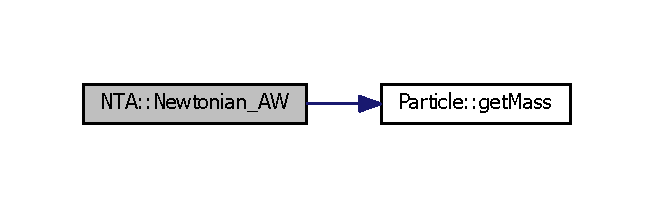
\includegraphics[width=314pt]{namespaceNTA_aad37ae368f0a920088e180a73187685a_cgraph}
\end{center}
\end{figure}
\hypertarget{namespaceNTA_a5b1a4fcaa09041cdf89a6b3122815c56}{}\label{namespaceNTA_a5b1a4fcaa09041cdf89a6b3122815c56} 
\index{N\+TA@{N\+TA}!Newtonian\+\_\+ext\+Acc@{Newtonian\+\_\+ext\+Acc}}
\index{Newtonian\+\_\+ext\+Acc@{Newtonian\+\_\+ext\+Acc}!N\+TA@{N\+TA}}
\subsubsection{\texorpdfstring{Newtonian\+\_\+ext\+Acc()}{Newtonian\_extAcc()}}
{\footnotesize\ttfamily void N\+T\+A\+::\+Newtonian\+\_\+ext\+Acc (\begin{DoxyParamCaption}\item[{\hyperlink{namespaceNTA_a19ccaac066849b26305dbbbee129fa0e}{double3} $\ast$}]{acc,  }\item[{const double}]{t,  }\item[{\hyperlink{classParticle}{Particle} $\ast$}]{p,  }\item[{const int}]{np,  }\item[{\hyperlink{classParticle}{Particle} $\ast$}]{pert,  }\item[{\hyperlink{namespaceNTA_a19ccaac066849b26305dbbbee129fa0e}{double3} $\ast$}]{pertf,  }\item[{const int}]{npert,  }\item[{\hyperlink{classNTA_1_1Newtonian__pars}{Newtonian\+\_\+pars} $\ast$}]{pars }\end{DoxyParamCaption})}



Newtonian acceleration from perturber pert to particle p (function type of \hyperlink{namespaceARC_a7aeda3b3bd009af7ac964748834dd312}{A\+R\+C\+::ext\+\_\+\+Acc}) 


\begin{DoxyParams}[1]{Parameters}
\mbox{\tt out}  & {\em acc} & acceleration vector from pert to p. $ \sum_j Aij[1:3] = m_i m_p (xp[1:3]-xi[1:3]) / |xp-xi|^3 $. \\
\hline
\mbox{\tt in}  & {\em t} & time step for prediction of pert particles \\
\hline
\mbox{\tt in}  & {\em p} & particle array \\
\hline
\mbox{\tt in}  & {\em np} & number of particles \\
\hline
\mbox{\tt in}  & {\em pert} & perturber particle array \\
\hline
\mbox{\tt in}  & {\em pertf} & perturrber force array for prediction \\
\hline
\mbox{\tt in}  & {\em npert} & number of perturbers \\
\hline
\mbox{\tt in}  & {\em pars} & extra parameters (not used) \\
\hline
\end{DoxyParams}
Here is the call graph for this function\+:
\nopagebreak
\begin{figure}[H]
\begin{center}
\leavevmode
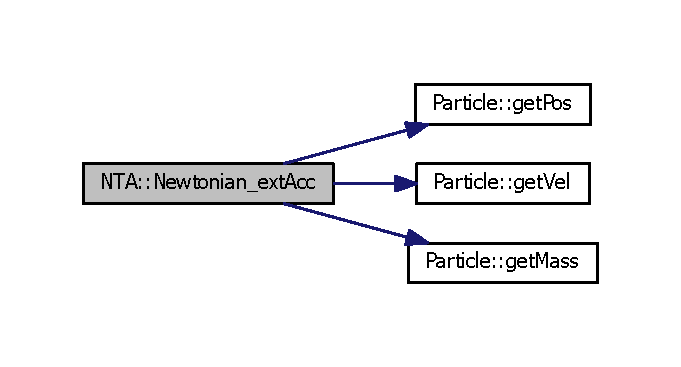
\includegraphics[width=327pt]{namespaceNTA_a5b1a4fcaa09041cdf89a6b3122815c56_cgraph}
\end{center}
\end{figure}
\hypertarget{namespaceNTA_a5125fd91a773d67901c4e0f8896e3dca}{}\label{namespaceNTA_a5125fd91a773d67901c4e0f8896e3dca} 
\index{N\+TA@{N\+TA}!Newtonian\+\_\+kepler\+\_\+period@{Newtonian\+\_\+kepler\+\_\+period}}
\index{Newtonian\+\_\+kepler\+\_\+period@{Newtonian\+\_\+kepler\+\_\+period}!N\+TA@{N\+TA}}
\subsubsection{\texorpdfstring{Newtonian\+\_\+kepler\+\_\+period()}{Newtonian\_kepler\_period()}}
{\footnotesize\ttfamily double N\+T\+A\+::\+Newtonian\+\_\+kepler\+\_\+period (\begin{DoxyParamCaption}\item[{const double}]{m1,  }\item[{const double}]{m2,  }\item[{const double}]{dx\mbox{[}3\mbox{]},  }\item[{const double}]{dv\mbox{[}3\mbox{]},  }\item[{\hyperlink{classNTA_1_1Newtonian__pars}{Newtonian\+\_\+pars} $\ast$}]{pars }\end{DoxyParamCaption})}



Newtonian two-\/body kepler period. 

Use \hyperlink{namespaceNTA_a02d22f02e21004b264c8257a5ffbb600}{calc\+\_\+kepler\+\_\+orbit\+\_\+par()} to obtain the two-\/body kepler period 
\begin{DoxyParams}[1]{Parameters}
\mbox{\tt in}  & {\em m1} & mass of particle 1 \\
\hline
\mbox{\tt in}  & {\em m2} & mass of particle 2 \\
\hline
\mbox{\tt in}  & {\em dx} & relative position vector \\
\hline
\mbox{\tt in}  & {\em dv} & relative velocity vector \\
\hline
\mbox{\tt in}  & {\em pars} & \hyperlink{classNTA_1_1Newtonian__pars}{Newtonian\+\_\+pars} type data (not used) \\
\hline
\end{DoxyParams}
\begin{DoxyReturn}{Returns}
If the orbit is close, return the period, otherwise return the approximately 10\% of free-\/fall time. 
\end{DoxyReturn}

\chapter{Class Documentation}
\hypertarget{classARC_1_1chain}{}\section{A\+RC\+:\+:chain$<$ particle, int\+\_\+par $>$ Class Template Reference}
\label{classARC_1_1chain}\index{A\+R\+C\+::chain$<$ particle, int\+\_\+par $>$@{A\+R\+C\+::chain$<$ particle, int\+\_\+par $>$}}


\hyperlink{namespaceARC}{A\+RC} class based on template class particle.  




{\ttfamily \#include $<$A\+R.\+h$>$}



Collaboration diagram for A\+RC\+:\+:chain$<$ particle, int\+\_\+par $>$\+:
\nopagebreak
\begin{figure}[H]
\begin{center}
\leavevmode
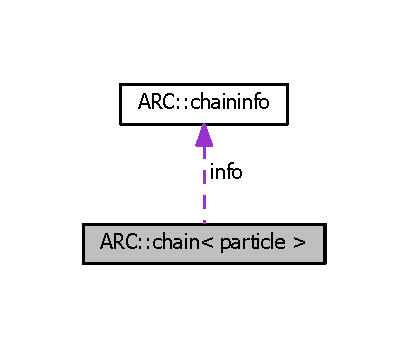
\includegraphics[width=189pt]{classARC_1_1chain__coll__graph}
\end{center}
\end{figure}
\subsection*{Public Member Functions}
\begin{DoxyCompactItemize}
\item 
\hyperlink{classARC_1_1chain_af5c20ba1cd4cbefc736e1df84962dbe1}{chain} (const std\+::size\+\_\+t n, const \hyperlink{classARC_1_1chainpars}{chainpars}$<$ int\+\_\+par $>$ \&par)
\begin{DoxyCompactList}\small\item\em Constructor. \end{DoxyCompactList}\item 
\hyperlink{classARC_1_1chain_a5f8a260f762232ba4a823de1815416ef}{chain} (const \hyperlink{classARC_1_1chainpars}{chainpars}$<$ int\+\_\+par $>$ \&par)
\begin{DoxyCompactList}\small\item\em Constructor. \end{DoxyCompactList}\item 
void \hyperlink{classARC_1_1chain_a0c3c1daffa75873b39d9964eebc6566f}{allocate} (const std\+::size\+\_\+t n)
\begin{DoxyCompactList}\small\item\em Allocate memory. \end{DoxyCompactList}\item 
void \hyperlink{classARC_1_1chain_a61d47f9599d4f7176b8870f825305011}{clear} ()
\begin{DoxyCompactList}\small\item\em Clear function. \end{DoxyCompactList}\item 
\hyperlink{classARC_1_1chain_a4e9c6711eb95c5614cd28b14d33ec3eb}{$\sim$chain} ()
\begin{DoxyCompactList}\small\item\em destructor \end{DoxyCompactList}\item 
double \hyperlink{classARC_1_1chain_a7e4f81985bb88e0fb0fcc739b9790396}{find\+\_\+strong\+\_\+pair} (int pindex\mbox{[}2\mbox{]})
\begin{DoxyCompactList}\small\item\em Find the most strongly interacted pair. \end{DoxyCompactList}\item 
double \hyperlink{classARC_1_1chain_a0c0cadba6cebb17e4d55b40ac98a608a}{find\+\_\+closest\+\_\+pair} (int pindex\mbox{[}2\mbox{]})
\begin{DoxyCompactList}\small\item\em Find the closest pair. \end{DoxyCompactList}\item 
double \hyperlink{classARC_1_1chain_a146941e5213125cc4a1c30622eed4568}{calc\+\_\+dt\+\_\+X} (const double ds)
\begin{DoxyCompactList}\small\item\em Calculate physical time step for X. \end{DoxyCompactList}\item 
double \hyperlink{classARC_1_1chain_a1453e04d5f3e15c51cca5de13832732d}{calc\+\_\+dt\+\_\+V} (const double ds)
\begin{DoxyCompactList}\small\item\em Calculate physical time step for V. \end{DoxyCompactList}\item 
double \hyperlink{classARC_1_1chain_a282545e539f7402b1d44bf285730490a}{calc\+\_\+next\+\_\+step\+\_\+\+X\+VA} ()
\begin{DoxyCompactList}\small\item\em Calculate next step approximation based on min(X/(gV),V/(gA)) \end{DoxyCompactList}\item 
double \hyperlink{classARC_1_1chain_ab3984977684a6ca9bf2214cd957f56a0}{calc\+\_\+next\+\_\+step\+\_\+custom} ()
\begin{DoxyCompactList}\small\item\em Calculate next step approximation based on custom defined timescale for two-\/body system. \end{DoxyCompactList}\item 
void \hyperlink{classARC_1_1chain_a6af4a9c65329265a45f0210c104fa96a}{addP} (particle \&a)
\begin{DoxyCompactList}\small\item\em Add particle. \end{DoxyCompactList}\item 
void \hyperlink{classARC_1_1chain_abf446295cee9e550c32d64e575f68d04}{addP} (\hyperlink{classARC_1_1chain}{chain}$<$ particle, int\+\_\+par $>$ \&a)
\begin{DoxyCompactList}\small\item\em Add chain as a particle in \#p. \end{DoxyCompactList}\item 
void \hyperlink{classARC_1_1chain_a2cd246cb307b8f04766c625de851ff52}{addP} (const std\+::size\+\_\+t n, particle a\mbox{[}$\,$\mbox{]})
\begin{DoxyCompactList}\small\item\em Add a list of particle. \end{DoxyCompactList}\item 
void \hyperlink{classARC_1_1chain_a450a7459b076331b6aaa888d209e888c}{removeP} (const std\+::size\+\_\+t i, bool option=true)
\begin{DoxyCompactList}\small\item\em remove one particle \end{DoxyCompactList}\item 
void \hyperlink{classARC_1_1chain_a6b7202e64c0a4f5d4f3f8a31f9d27e20}{dump} (const char $\ast$filename)
\begin{DoxyCompactList}\small\item\em Data Dumping to file function. \end{DoxyCompactList}\item 
void \hyperlink{classARC_1_1chain_a921a250cfcfe7a5b8e597ddcb03730ec}{load} (const char $\ast$filename)
\begin{DoxyCompactList}\small\item\em Data reading from file function. \end{DoxyCompactList}\item 
void \hyperlink{classARC_1_1chain_ae14cbd0c85aa090d0848538c6eae0afd}{readP} (const char $\ast$filename)
\begin{DoxyCompactList}\small\item\em Read particle data from file. \end{DoxyCompactList}\item 
void \hyperlink{classARC_1_1chain_a1c6de84a911feff1425dfb59e7a89087}{init\+Pext} (const std\+::size\+\_\+t n)
\begin{DoxyCompactList}\small\item\em Allocate memory for perturber list. \end{DoxyCompactList}\item 
void \hyperlink{classARC_1_1chain_ab6892980b326bd0bbe8a873a71892801}{add\+Pext} (particle \&a)
\begin{DoxyCompactList}\small\item\em Add one perturber particle. \end{DoxyCompactList}\item 
void \hyperlink{classARC_1_1chain_a964e4afb654f3d380969aa2326a287cc}{add\+Pext} (\hyperlink{classARC_1_1chain}{chain}$<$ particle, int\+\_\+par $>$ \&a)
\begin{DoxyCompactList}\small\item\em Add one chain as a perturber particle. \end{DoxyCompactList}\item 
void \hyperlink{classARC_1_1chain_a6b5cf35f505262d9d2326abb2904d91d}{add\+Pext} (const std\+::size\+\_\+t n, particle a\mbox{[}$\,$\mbox{]})
\begin{DoxyCompactList}\small\item\em Add a list of perturber particles. \end{DoxyCompactList}\item 
void \hyperlink{classARC_1_1chain_a7d563413beb44795b8ecd1348a2d2305}{remove\+Pext} (const std\+::size\+\_\+t i, bool option=true)
\begin{DoxyCompactList}\small\item\em Remove one perturber. \end{DoxyCompactList}\item 
bool \hyperlink{classARC_1_1chain_a29ff9707fe94a554966c885d9bafa819}{is\+Pmod} () const
\begin{DoxyCompactList}\small\item\em Indicator of changes in particle list \#p. \end{DoxyCompactList}\item 
int \hyperlink{classARC_1_1chain_a7de218a1874b150ee44a05aa9d7b7b6d}{is\+Porigin} () const
\begin{DoxyCompactList}\small\item\em Indicator of particle frame. \end{DoxyCompactList}\item 
const particle \& \hyperlink{classARC_1_1chain_ad8bacf5ad6ea0bb31bdb457e4c626701}{getP} (const std\+::size\+\_\+t i) const
\begin{DoxyCompactList}\small\item\em Get particle i (const reference) \end{DoxyCompactList}\item 
const particle \& \hyperlink{classARC_1_1chain_a992795e009faf43b59fc338350ae210c}{get\+Pext} (const std\+::size\+\_\+t i) const
\begin{DoxyCompactList}\small\item\em Get pertuber particle i (const reference) \end{DoxyCompactList}\item 
const int \hyperlink{classARC_1_1chain_a582ad9ae8003400e06bba908d70d60d9}{getN} () const
\begin{DoxyCompactList}\small\item\em Get current number of chain members. \end{DoxyCompactList}\item 
void \hyperlink{classARC_1_1chain_a3fe37720ceb48c14905c92d3e25e71a4}{init} (const double time)
\begin{DoxyCompactList}\small\item\em Initialization. \end{DoxyCompactList}\item 
void \hyperlink{classARC_1_1chain_a34cb0bde571c3d8cc8204c3e7c11a821}{link\+\_\+int\+\_\+par} (int\+\_\+par \&par)
\begin{DoxyCompactList}\small\item\em link interaction parameter class \end{DoxyCompactList}\item 
int\+\_\+par \& \hyperlink{classARC_1_1chain_af9bdf54999606c0d6f32843f0d53d8c4}{get\+\_\+int\+\_\+par} ()
\begin{DoxyCompactList}\small\item\em Get interaction parameter. \end{DoxyCompactList}\item 
void \hyperlink{classARC_1_1chain_a7bd0d1b03bcc2e7cdb146960e9d55ea3}{center\+\_\+shift\+\_\+inverse} ()
\begin{DoxyCompactList}\small\item\em Inversed center-\/of-\/mass frame shift for particles. \end{DoxyCompactList}\item 
void \hyperlink{classARC_1_1chain_a73419f14f724668f4858a13c01cf7b70}{center\+\_\+shift} ()
\begin{DoxyCompactList}\small\item\em Center-\/of-\/mass frame shift for particles. \end{DoxyCompactList}\item 
void \hyperlink{classARC_1_1chain_ad098493cd057ac19786f5bc85f9ab25d}{backup} (double $\ast$db)
\begin{DoxyCompactList}\small\item\em Backup chain data (\#t, \#\+Pt, \#w, \#X, \#V) \end{DoxyCompactList}\item 
void \hyperlink{classARC_1_1chain_a5b1bec1324def99667dc6783108d1607}{restore} (double $\ast$db)
\begin{DoxyCompactList}\small\item\em Restore chain data (\#t, \#\+Pt, \#w, \#X, \#V) \end{DoxyCompactList}\item 
void \hyperlink{classARC_1_1chain_aff3cd92c840d1bbbc903a8a07eb079d0}{Leapfrog\+\_\+step\+\_\+forward} (const double s, const int n, const double3 $\ast$force=N\+U\+LL, int check\+\_\+flag=1, double $\ast$$\ast$dpoly=N\+U\+LL, const int ndmax=0)
\begin{DoxyCompactList}\small\item\em Leapfrog integrator. \end{DoxyCompactList}\item 
double \hyperlink{classARC_1_1chain_ae4d0002cceee2397101a43b3755f927e}{extrapolation\+\_\+integration} (const double ds, const double toff=-\/1.\+0, const double3 $\ast$force=N\+U\+LL, const bool err\+\_\+ignore=false)
\begin{DoxyCompactList}\small\item\em Extrapolation integration. \end{DoxyCompactList}\item 
double \hyperlink{classARC_1_1chain_ad21bc515c01cf62e65d6d749d8babd63}{get\+Time} () const
\begin{DoxyCompactList}\small\item\em Get current physical time. \end{DoxyCompactList}\item 
double \hyperlink{classARC_1_1chain_aec4fe3207a5fe2d0a254bdd4bb54ae7f}{get\+Ekin} () const
\begin{DoxyCompactList}\small\item\em Get current kinetic energy. \end{DoxyCompactList}\item 
double \hyperlink{classARC_1_1chain_ade5db39891ff7a2d10ac38786ab866c1}{get\+Pot} () const
\begin{DoxyCompactList}\small\item\em Get current potential energy. \end{DoxyCompactList}\item 
double \hyperlink{classARC_1_1chain_a1404204bd5665aa2d12d57cf653b779c}{get\+Pt} () const
\begin{DoxyCompactList}\small\item\em Get current time momemtum $Pt$ (current system binding energy) \end{DoxyCompactList}\item 
double \hyperlink{classARC_1_1chain_abdd62eb43e4a7b5eca10190c90ed190f}{getw} () const
\begin{DoxyCompactList}\small\item\em Get current integrated time transformation function value $w$. \end{DoxyCompactList}\item 
double \hyperlink{classARC_1_1chain_abcfc20c1694a1d68a324ea9a08863af3}{getW} () const
\begin{DoxyCompactList}\small\item\em Get current time transformation function value $W$. \end{DoxyCompactList}\item 
void \hyperlink{classARC_1_1chain_a5e5a7da2a07800be47623794fe6fe44d}{get\+List} (std\+::size\+\_\+t $\ast$indexlist)
\begin{DoxyCompactList}\small\item\em Get chain list. \end{DoxyCompactList}\item 
void \hyperlink{classARC_1_1chain_a4624cf80ecb8804bc08fb7f23fdddb4e}{print} (std\+::ostream \&fout, const int precision=15, const int width=15)
\begin{DoxyCompactList}\small\item\em print chain data \end{DoxyCompactList}\end{DoxyCompactItemize}
\subsection*{Public Attributes}
\begin{DoxyCompactItemize}
\item 
particle \hyperlink{classARC_1_1chain_a2eead75bd916fa7ffc05341645527847}{cm}
\begin{DoxyCompactList}\small\item\em center mass particle \end{DoxyCompactList}\item 
\hyperlink{classARC_1_1chaininfo}{chaininfo} $\ast$ \hyperlink{classARC_1_1chain_a7ad20a60e038d16522c11d7fccb47648}{info}
\begin{DoxyCompactList}\small\item\em chain information \end{DoxyCompactList}\end{DoxyCompactItemize}


\subsection{Detailed Description}
\subsubsection*{template$<$class particle, class int\+\_\+par$>$\newline
class A\+R\+C\+::chain$<$ particle, int\+\_\+par $>$}

\hyperlink{namespaceARC}{A\+RC} class based on template class particle. 

Major class for \hyperlink{namespaceARC}{A\+RC} integration of few bodies

It depend on the template class particle. This particle class should contain public member functions for reading and writing mass, position and velocity (see sample in \hyperlink{classParticle_a97d76b66aed57834c105b78b10643b81}{Particle\+::set\+Pos()}, \hyperlink{classParticle_a07c405254ac3f03854e7523ff473c828}{Particle\+::set\+Vel()}, \hyperlink{classParticle_a620f479862b90468a77da4e9cf5c0ff5}{Particle\+::set\+Mass()}, \hyperlink{classParticle_a4ec76421cddd91b1f27357fb182f6923}{Particle\+::get\+Pos()}, \hyperlink{classParticle_ab3d63df7f8c22f232b096ae33b6ea3ac}{Particle\+::get\+Vel()}, \hyperlink{classParticle_a2576aff503f68e78ced91406512b1255}{Particle\+::get\+Mass()}) The template depended type int\+\_\+par is user-\/defined class for two-\/body interations used in \hyperlink{classARC_1_1chainpars_a9558124278a55c0301642e1df63be063}{A\+R\+C\+::chainpars.\+pair\+\_\+\+AW}, \hyperlink{classARC_1_1chainpars_a80fcc6e3b5ce69025126bc49d90f233c}{A\+R\+C\+::chainpars.\+pair\+\_\+\+Ap}

The basic way to use \hyperlink{namespaceARC}{A\+RC} integration is shown as following\+:
\begin{DoxyEnumerate}
\item Construct a chain class with template class particle and a parameter controller of \hyperlink{classARC_1_1chainpars}{A\+R\+C\+::chainpars}. (The \hyperlink{classARC_1_1chainpars}{A\+R\+C\+::chainpars} should be configured first before doing integration. see its document for detail).
\item Add existed particle \textquotesingle{}A\textquotesingle{} (or a list of particles, or a chain type particle) into chain particle list (chain.\+p) using \hyperlink{classARC_1_1chain_a6af4a9c65329265a45f0210c104fa96a}{chain.\+add\+P()}. Notice the \hyperlink{classARC_1_1chain_a6af4a9c65329265a45f0210c104fa96a}{chain.\+add\+P()} only registers the particle A\textquotesingle{}s memory address into chain.\+p without copying data. The chain integration will directly modify the position and velocity of particle A.
\item Add perturbers into chain perturber list (chain.\+pext) using \hyperlink{classARC_1_1chain_ab6892980b326bd0bbe8a873a71892801}{chain.\+add\+Pext()} (also only register the particle address)
\item Initialize Int\+\_\+pars used for \+::\+A\+R\+C\+::pair\+\_\+\+AW or \+::\+A\+R\+C\+::pair\+\_\+\+Ap if necessary (see the case of \hyperlink{namespaceNTA_aecd205ef07c4302cd04d04218c4426e6}{A\+R\+C\+::\+Newtonian\+\_\+\+A\+W()})
\item Initialize chain with \hyperlink{classARC_1_1chain_a3fe37720ceb48c14905c92d3e25e71a4}{chain.\+init()}. Notice this function is necessary to be called before integration. Also be careful that after this initialization, the positions and velocites of particles registered in chain.\+p will be shifted from their original frame to their center-\/of-\/mass frame. The particle type member variable \hyperlink{classARC_1_1chain_a2eead75bd916fa7ffc05341645527847}{chain\+::cm} stores the center-\/of-\/mass data of these particles (the mass of \hyperlink{classARC_1_1chain_a2eead75bd916fa7ffc05341645527847}{chain\+::cm} is the total mass of all member particles).
\item Call integration functions (\hyperlink{classARC_1_1chain_aff3cd92c840d1bbbc903a8a07eb079d0}{chain.\+Leapfrog\+\_\+step\+\_\+forward()} or \hyperlink{classARC_1_1chain_ae4d0002cceee2397101a43b3755f927e}{chain.\+extrapolation\+\_\+integration()}). The former use only Leapfrog method and the latter use extrapolation method to obtain high accuracy of integration.
\item After call integration functions, the particles are integrated to new time. Because in \hyperlink{namespaceARC}{A\+RC} method, the time is also integrated and cannot be predicted before integration, thus the iteration need to be done to get correct physical time you want (see detailed in \hyperlink{classARC_1_1chain_ae4d0002cceee2397101a43b3755f927e}{chain.\+extrapolation\+\_\+integration()} document).
\item Notice that after \hyperlink{classARC_1_1chain_a3fe37720ceb48c14905c92d3e25e71a4}{chain.\+init()} and integration, the particles are always in the center-\/of-\/mass frame. If you want to shift them back to the original frame, the \hyperlink{classARC_1_1chain_a7bd0d1b03bcc2e7cdb146960e9d55ea3}{chain.\+center\+\_\+shift\+\_\+inverse()} should be used. But after this function is used, you should use \hyperlink{classARC_1_1chain_a73419f14f724668f4858a13c01cf7b70}{chain.\+center\+\_\+shift()} before the next integration.
\end{DoxyEnumerate}

Because of time now is an integrated variable, the time after integration cannot be predicted. Thus if you want to stop the integration at a certain physical time, you need to use \hyperlink{classARC_1_1chain_ae4d0002cceee2397101a43b3755f927e}{chain.\+extrapolation\+\_\+integration()} with dense output. To get better accuracy of physical time from intepolation, the 4k sequences (set in chainpars.\+set\+E\+X\+P()) is strongly suggested to be used. If 4k sequences are used, the dense output method for G\+BS is used and the accuracy of time intepolation is close to the accuracy of integration. Please check the document of \hyperlink{classARC_1_1chain_ae4d0002cceee2397101a43b3755f927e}{chain.\+extrapolation\+\_\+integration()} for detail. 

\subsection{Constructor \& Destructor Documentation}
\hypertarget{classARC_1_1chain_af5c20ba1cd4cbefc736e1df84962dbe1}{}\label{classARC_1_1chain_af5c20ba1cd4cbefc736e1df84962dbe1} 
\index{A\+R\+C\+::chain@{A\+R\+C\+::chain}!chain@{chain}}
\index{chain@{chain}!A\+R\+C\+::chain@{A\+R\+C\+::chain}}
\subsubsection{\texorpdfstring{chain()}{chain()}\hspace{0.1cm}{\footnotesize\ttfamily [1/2]}}
{\footnotesize\ttfamily template$<$class particle, class int\+\_\+par$>$ \\
\hyperlink{classARC_1_1chain}{A\+R\+C\+::chain}$<$ particle, int\+\_\+par $>$\+::\hyperlink{classARC_1_1chain}{chain} (\begin{DoxyParamCaption}\item[{const std\+::size\+\_\+t}]{n,  }\item[{const \hyperlink{classARC_1_1chainpars}{chainpars}$<$ int\+\_\+par $>$ \&}]{par }\end{DoxyParamCaption})\hspace{0.3cm}{\ttfamily [inline]}}



Constructor. 

Construct chain with allocated memory 
\begin{DoxyParams}[1]{Parameters}
\mbox{\tt in}  & {\em n} & maximum number of particles (will be used to allocate memory) \\
\hline
\mbox{\tt in}  & {\em par} & chain option controller class \hyperlink{classARC_1_1chainpars}{A\+R\+C\+::chainpars} \\
\hline
\end{DoxyParams}
\hypertarget{classARC_1_1chain_a5f8a260f762232ba4a823de1815416ef}{}\label{classARC_1_1chain_a5f8a260f762232ba4a823de1815416ef} 
\index{A\+R\+C\+::chain@{A\+R\+C\+::chain}!chain@{chain}}
\index{chain@{chain}!A\+R\+C\+::chain@{A\+R\+C\+::chain}}
\subsubsection{\texorpdfstring{chain()}{chain()}\hspace{0.1cm}{\footnotesize\ttfamily [2/2]}}
{\footnotesize\ttfamily template$<$class particle, class int\+\_\+par$>$ \\
\hyperlink{classARC_1_1chain}{A\+R\+C\+::chain}$<$ particle, int\+\_\+par $>$\+::\hyperlink{classARC_1_1chain}{chain} (\begin{DoxyParamCaption}\item[{const \hyperlink{classARC_1_1chainpars}{chainpars}$<$ int\+\_\+par $>$ \&}]{par }\end{DoxyParamCaption})\hspace{0.3cm}{\ttfamily [inline]}}



Constructor. 

Construct chain without memory allocate, need to call \hyperlink{classARC_1_1chain_a0c3c1daffa75873b39d9964eebc6566f}{allocate()} later. 
\begin{DoxyParams}[1]{Parameters}
\mbox{\tt in}  & {\em par} & chain option controller class \hyperlink{classARC_1_1chainpars}{A\+R\+C\+::chainpars} \\
\hline
\end{DoxyParams}
\hypertarget{classARC_1_1chain_a4e9c6711eb95c5614cd28b14d33ec3eb}{}\label{classARC_1_1chain_a4e9c6711eb95c5614cd28b14d33ec3eb} 
\index{A\+R\+C\+::chain@{A\+R\+C\+::chain}!````~chain@{$\sim$chain}}
\index{````~chain@{$\sim$chain}!A\+R\+C\+::chain@{A\+R\+C\+::chain}}
\subsubsection{\texorpdfstring{$\sim$chain()}{~chain()}}
{\footnotesize\ttfamily template$<$class particle, class int\+\_\+par$>$ \\
\hyperlink{classARC_1_1chain}{A\+R\+C\+::chain}$<$ particle, int\+\_\+par $>$\+::$\sim$\hyperlink{classARC_1_1chain}{chain} (\begin{DoxyParamCaption}{ }\end{DoxyParamCaption})\hspace{0.3cm}{\ttfamily [inline]}}



destructor 

Here is the call graph for this function\+:
\nopagebreak
\begin{figure}[H]
\begin{center}
\leavevmode
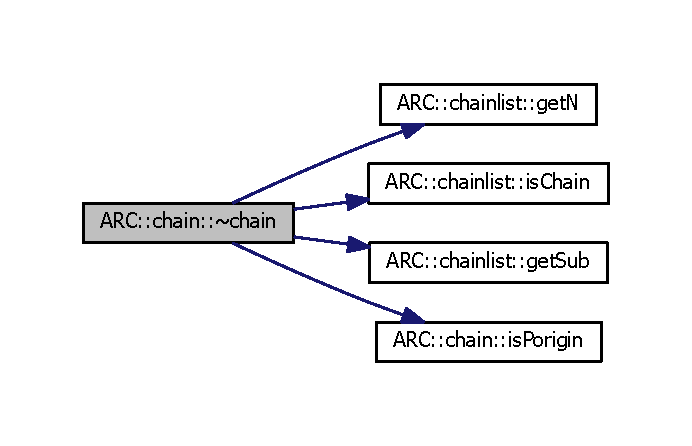
\includegraphics[width=332pt]{classARC_1_1chain_a4e9c6711eb95c5614cd28b14d33ec3eb_cgraph}
\end{center}
\end{figure}


\subsection{Member Function Documentation}
\hypertarget{classARC_1_1chain_a6af4a9c65329265a45f0210c104fa96a}{}\label{classARC_1_1chain_a6af4a9c65329265a45f0210c104fa96a} 
\index{A\+R\+C\+::chain@{A\+R\+C\+::chain}!addP@{addP}}
\index{addP@{addP}!A\+R\+C\+::chain@{A\+R\+C\+::chain}}
\subsubsection{\texorpdfstring{add\+P()}{addP()}\hspace{0.1cm}{\footnotesize\ttfamily [1/3]}}
{\footnotesize\ttfamily template$<$class particle, class int\+\_\+par$>$ \\
void \hyperlink{classARC_1_1chain}{A\+R\+C\+::chain}$<$ particle, int\+\_\+par $>$\+::addP (\begin{DoxyParamCaption}\item[{particle \&}]{a }\end{DoxyParamCaption})\hspace{0.3cm}{\ttfamily [inline]}}



Add particle. 

Add one particle (address pointer) into particle list \#p (see \hyperlink{classARC_1_1chainlist_ab04a5742cd27168e0404e57a67d6afd1}{A\+R\+C\+::chainlist.\+add()}) 
\begin{DoxyParams}[1]{Parameters}
\mbox{\tt in}  & {\em a} & new particle \\
\hline
\end{DoxyParams}
Here is the call graph for this function\+:
\nopagebreak
\begin{figure}[H]
\begin{center}
\leavevmode
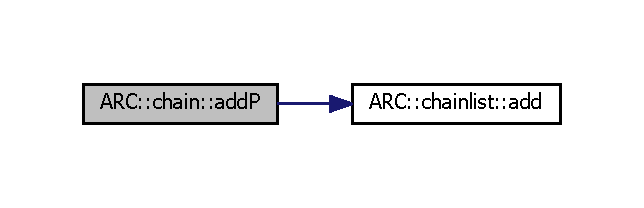
\includegraphics[width=309pt]{classARC_1_1chain_a6af4a9c65329265a45f0210c104fa96a_cgraph}
\end{center}
\end{figure}
\hypertarget{classARC_1_1chain_abf446295cee9e550c32d64e575f68d04}{}\label{classARC_1_1chain_abf446295cee9e550c32d64e575f68d04} 
\index{A\+R\+C\+::chain@{A\+R\+C\+::chain}!addP@{addP}}
\index{addP@{addP}!A\+R\+C\+::chain@{A\+R\+C\+::chain}}
\subsubsection{\texorpdfstring{add\+P()}{addP()}\hspace{0.1cm}{\footnotesize\ttfamily [2/3]}}
{\footnotesize\ttfamily template$<$class particle, class int\+\_\+par$>$ \\
void \hyperlink{classARC_1_1chain}{A\+R\+C\+::chain}$<$ particle, int\+\_\+par $>$\+::addP (\begin{DoxyParamCaption}\item[{\hyperlink{classARC_1_1chain}{chain}$<$ particle, int\+\_\+par $>$ \&}]{a }\end{DoxyParamCaption})\hspace{0.3cm}{\ttfamily [inline]}}



Add chain as a particle in \#p. 

Add one chain (address pointer) into particle list \#p (see \hyperlink{classARC_1_1chainlist_ab04a5742cd27168e0404e57a67d6afd1}{A\+R\+C\+::chainlist.\+add()}) 
\begin{DoxyParams}[1]{Parameters}
\mbox{\tt in}  & {\em a} & new chain particle \\
\hline
\end{DoxyParams}
Here is the call graph for this function\+:
\nopagebreak
\begin{figure}[H]
\begin{center}
\leavevmode
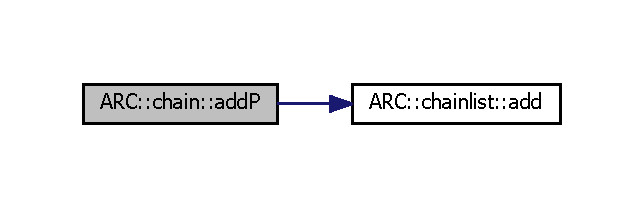
\includegraphics[width=309pt]{classARC_1_1chain_abf446295cee9e550c32d64e575f68d04_cgraph}
\end{center}
\end{figure}
\hypertarget{classARC_1_1chain_a2cd246cb307b8f04766c625de851ff52}{}\label{classARC_1_1chain_a2cd246cb307b8f04766c625de851ff52} 
\index{A\+R\+C\+::chain@{A\+R\+C\+::chain}!addP@{addP}}
\index{addP@{addP}!A\+R\+C\+::chain@{A\+R\+C\+::chain}}
\subsubsection{\texorpdfstring{add\+P()}{addP()}\hspace{0.1cm}{\footnotesize\ttfamily [3/3]}}
{\footnotesize\ttfamily template$<$class particle, class int\+\_\+par$>$ \\
void \hyperlink{classARC_1_1chain}{A\+R\+C\+::chain}$<$ particle, int\+\_\+par $>$\+::addP (\begin{DoxyParamCaption}\item[{const std\+::size\+\_\+t}]{n,  }\item[{particle}]{a\mbox{[}$\,$\mbox{]} }\end{DoxyParamCaption})\hspace{0.3cm}{\ttfamily [inline]}}



Add a list of particle. 

Add a list of particles (see \hyperlink{classARC_1_1chainlist_ab04a5742cd27168e0404e57a67d6afd1}{A\+R\+C\+::chainlist.\+add()}) 
\begin{DoxyParams}[1]{Parameters}
\mbox{\tt in}  & {\em n} & number of particles need to be added \\
\hline
\mbox{\tt in}  & {\em a} & array of new particles \\
\hline
\end{DoxyParams}
Here is the call graph for this function\+:
\nopagebreak
\begin{figure}[H]
\begin{center}
\leavevmode
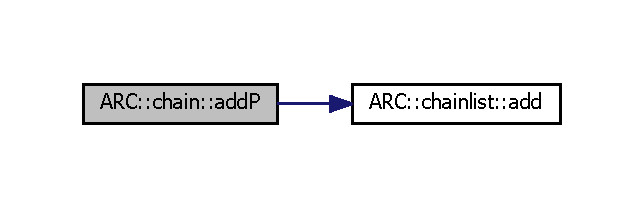
\includegraphics[width=309pt]{classARC_1_1chain_a2cd246cb307b8f04766c625de851ff52_cgraph}
\end{center}
\end{figure}
\hypertarget{classARC_1_1chain_ab6892980b326bd0bbe8a873a71892801}{}\label{classARC_1_1chain_ab6892980b326bd0bbe8a873a71892801} 
\index{A\+R\+C\+::chain@{A\+R\+C\+::chain}!add\+Pext@{add\+Pext}}
\index{add\+Pext@{add\+Pext}!A\+R\+C\+::chain@{A\+R\+C\+::chain}}
\subsubsection{\texorpdfstring{add\+Pext()}{addPext()}\hspace{0.1cm}{\footnotesize\ttfamily [1/3]}}
{\footnotesize\ttfamily template$<$class particle, class int\+\_\+par$>$ \\
void \hyperlink{classARC_1_1chain}{A\+R\+C\+::chain}$<$ particle, int\+\_\+par $>$\+::add\+Pext (\begin{DoxyParamCaption}\item[{particle \&}]{a }\end{DoxyParamCaption})\hspace{0.3cm}{\ttfamily [inline]}}



Add one perturber particle. 

Add one perturber particle (address pointer) into \#pext 
\begin{DoxyParams}[1]{Parameters}
\mbox{\tt in}  & {\em a} & perturber particle \\
\hline
\end{DoxyParams}
Here is the call graph for this function\+:
\nopagebreak
\begin{figure}[H]
\begin{center}
\leavevmode
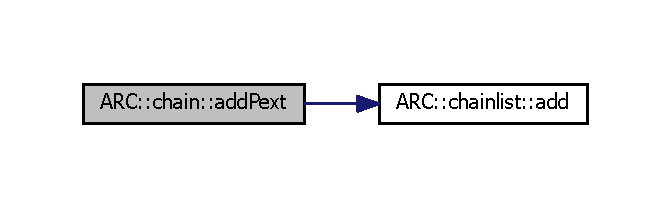
\includegraphics[width=322pt]{classARC_1_1chain_ab6892980b326bd0bbe8a873a71892801_cgraph}
\end{center}
\end{figure}
\hypertarget{classARC_1_1chain_a964e4afb654f3d380969aa2326a287cc}{}\label{classARC_1_1chain_a964e4afb654f3d380969aa2326a287cc} 
\index{A\+R\+C\+::chain@{A\+R\+C\+::chain}!add\+Pext@{add\+Pext}}
\index{add\+Pext@{add\+Pext}!A\+R\+C\+::chain@{A\+R\+C\+::chain}}
\subsubsection{\texorpdfstring{add\+Pext()}{addPext()}\hspace{0.1cm}{\footnotesize\ttfamily [2/3]}}
{\footnotesize\ttfamily template$<$class particle, class int\+\_\+par$>$ \\
void \hyperlink{classARC_1_1chain}{A\+R\+C\+::chain}$<$ particle, int\+\_\+par $>$\+::add\+Pext (\begin{DoxyParamCaption}\item[{\hyperlink{classARC_1_1chain}{chain}$<$ particle, int\+\_\+par $>$ \&}]{a }\end{DoxyParamCaption})\hspace{0.3cm}{\ttfamily [inline]}}



Add one chain as a perturber particle. 

Add one chain as a perturber particle (address pointer) into \#pext 
\begin{DoxyParams}[1]{Parameters}
\mbox{\tt in}  & {\em a} & the chain perturber \\
\hline
\end{DoxyParams}
Here is the call graph for this function\+:
\nopagebreak
\begin{figure}[H]
\begin{center}
\leavevmode
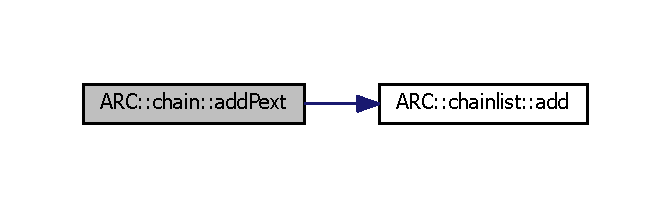
\includegraphics[width=322pt]{classARC_1_1chain_a964e4afb654f3d380969aa2326a287cc_cgraph}
\end{center}
\end{figure}
\hypertarget{classARC_1_1chain_a6b5cf35f505262d9d2326abb2904d91d}{}\label{classARC_1_1chain_a6b5cf35f505262d9d2326abb2904d91d} 
\index{A\+R\+C\+::chain@{A\+R\+C\+::chain}!add\+Pext@{add\+Pext}}
\index{add\+Pext@{add\+Pext}!A\+R\+C\+::chain@{A\+R\+C\+::chain}}
\subsubsection{\texorpdfstring{add\+Pext()}{addPext()}\hspace{0.1cm}{\footnotesize\ttfamily [3/3]}}
{\footnotesize\ttfamily template$<$class particle, class int\+\_\+par$>$ \\
void \hyperlink{classARC_1_1chain}{A\+R\+C\+::chain}$<$ particle, int\+\_\+par $>$\+::add\+Pext (\begin{DoxyParamCaption}\item[{const std\+::size\+\_\+t}]{n,  }\item[{particle}]{a\mbox{[}$\,$\mbox{]} }\end{DoxyParamCaption})\hspace{0.3cm}{\ttfamily [inline]}}



Add a list of perturber particles. 

Add a list of perturber particles (address pointer) into \#pext 
\begin{DoxyParams}[1]{Parameters}
\mbox{\tt in}  & {\em n} & number of particles need to be added \\
\hline
\mbox{\tt in}  & {\em a} & array of perturbers (address) \\
\hline
\end{DoxyParams}
Here is the call graph for this function\+:
\nopagebreak
\begin{figure}[H]
\begin{center}
\leavevmode
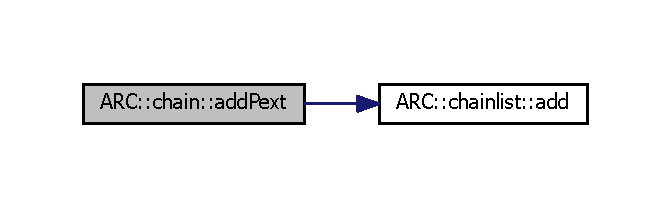
\includegraphics[width=322pt]{classARC_1_1chain_a6b5cf35f505262d9d2326abb2904d91d_cgraph}
\end{center}
\end{figure}
\hypertarget{classARC_1_1chain_a0c3c1daffa75873b39d9964eebc6566f}{}\label{classARC_1_1chain_a0c3c1daffa75873b39d9964eebc6566f} 
\index{A\+R\+C\+::chain@{A\+R\+C\+::chain}!allocate@{allocate}}
\index{allocate@{allocate}!A\+R\+C\+::chain@{A\+R\+C\+::chain}}
\subsubsection{\texorpdfstring{allocate()}{allocate()}}
{\footnotesize\ttfamily template$<$class particle, class int\+\_\+par$>$ \\
void \hyperlink{classARC_1_1chain}{A\+R\+C\+::chain}$<$ particle, int\+\_\+par $>$\+::allocate (\begin{DoxyParamCaption}\item[{const std\+::size\+\_\+t}]{n }\end{DoxyParamCaption})\hspace{0.3cm}{\ttfamily [inline]}}



Allocate memory. 

Allocate memory for maximum particle number n 
\begin{DoxyParams}[1]{Parameters}
\mbox{\tt in}  & {\em n} & maximum number of particles \\
\hline
\end{DoxyParams}
Here is the call graph for this function\+:
\nopagebreak
\begin{figure}[H]
\begin{center}
\leavevmode
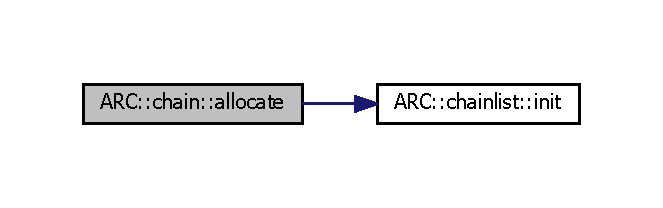
\includegraphics[width=318pt]{classARC_1_1chain_a0c3c1daffa75873b39d9964eebc6566f_cgraph}
\end{center}
\end{figure}
\hypertarget{classARC_1_1chain_ad098493cd057ac19786f5bc85f9ab25d}{}\label{classARC_1_1chain_ad098493cd057ac19786f5bc85f9ab25d} 
\index{A\+R\+C\+::chain@{A\+R\+C\+::chain}!backup@{backup}}
\index{backup@{backup}!A\+R\+C\+::chain@{A\+R\+C\+::chain}}
\subsubsection{\texorpdfstring{backup()}{backup()}}
{\footnotesize\ttfamily template$<$class particle, class int\+\_\+par$>$ \\
void \hyperlink{classARC_1_1chain}{A\+R\+C\+::chain}$<$ particle, int\+\_\+par $>$\+::backup (\begin{DoxyParamCaption}\item[{double $\ast$}]{db }\end{DoxyParamCaption})\hspace{0.3cm}{\ttfamily [inline]}}



Backup chain data (\#t, \#\+Pt, \#w, \#X, \#V) 

Backup chain data to one dimensional array.
\begin{DoxyItemize}
\item \#t \+: current physical time
\item \#\+Pt \+: current time momentum (system binding energy)
\item \#w \+: current time transformation parameter
\item \#X \+: current relative position array
\item \#V \+: current relative velocite array 
\begin{DoxyParams}[1]{Parameters}
\mbox{\tt out}  & {\em db} & backup array (size should be 6$\ast$\#num-\/3) where \#num is the total number of particles in \#p \\
\hline
\end{DoxyParams}

\end{DoxyItemize}\hypertarget{classARC_1_1chain_a1453e04d5f3e15c51cca5de13832732d}{}\label{classARC_1_1chain_a1453e04d5f3e15c51cca5de13832732d} 
\index{A\+R\+C\+::chain@{A\+R\+C\+::chain}!calc\+\_\+dt\+\_\+V@{calc\+\_\+dt\+\_\+V}}
\index{calc\+\_\+dt\+\_\+V@{calc\+\_\+dt\+\_\+V}!A\+R\+C\+::chain@{A\+R\+C\+::chain}}
\subsubsection{\texorpdfstring{calc\+\_\+dt\+\_\+\+V()}{calc\_dt\_V()}}
{\footnotesize\ttfamily template$<$class particle, class int\+\_\+par$>$ \\
double \hyperlink{classARC_1_1chain}{A\+R\+C\+::chain}$<$ particle, int\+\_\+par $>$\+::calc\+\_\+dt\+\_\+V (\begin{DoxyParamCaption}\item[{const double}]{ds }\end{DoxyParamCaption})\hspace{0.3cm}{\ttfamily [inline]}}



Calculate physical time step for V. 

Calculate physical time step dt for \#V based on ds 
\begin{DoxyParams}[1]{Parameters}
\mbox{\tt in}  & {\em ds} & step size s (not physical time step) \\
\hline
\end{DoxyParams}
\begin{DoxyReturn}{Returns}
dt\+: physical integration time step for \#V 
\end{DoxyReturn}
\hypertarget{classARC_1_1chain_a146941e5213125cc4a1c30622eed4568}{}\label{classARC_1_1chain_a146941e5213125cc4a1c30622eed4568} 
\index{A\+R\+C\+::chain@{A\+R\+C\+::chain}!calc\+\_\+dt\+\_\+X@{calc\+\_\+dt\+\_\+X}}
\index{calc\+\_\+dt\+\_\+X@{calc\+\_\+dt\+\_\+X}!A\+R\+C\+::chain@{A\+R\+C\+::chain}}
\subsubsection{\texorpdfstring{calc\+\_\+dt\+\_\+\+X()}{calc\_dt\_X()}}
{\footnotesize\ttfamily template$<$class particle, class int\+\_\+par$>$ \\
double \hyperlink{classARC_1_1chain}{A\+R\+C\+::chain}$<$ particle, int\+\_\+par $>$\+::calc\+\_\+dt\+\_\+X (\begin{DoxyParamCaption}\item[{const double}]{ds }\end{DoxyParamCaption})\hspace{0.3cm}{\ttfamily [inline]}}



Calculate physical time step for X. 

Calculate physical time step dt for \#X based on ds 
\begin{DoxyParams}[1]{Parameters}
\mbox{\tt in}  & {\em ds} & integration step size (not physical time step) \\
\hline
\end{DoxyParams}
\begin{DoxyReturn}{Returns}
dt\+: physical integration time step for \#X 
\end{DoxyReturn}
\hypertarget{classARC_1_1chain_ab3984977684a6ca9bf2214cd957f56a0}{}\label{classARC_1_1chain_ab3984977684a6ca9bf2214cd957f56a0} 
\index{A\+R\+C\+::chain@{A\+R\+C\+::chain}!calc\+\_\+next\+\_\+step\+\_\+custom@{calc\+\_\+next\+\_\+step\+\_\+custom}}
\index{calc\+\_\+next\+\_\+step\+\_\+custom@{calc\+\_\+next\+\_\+step\+\_\+custom}!A\+R\+C\+::chain@{A\+R\+C\+::chain}}
\subsubsection{\texorpdfstring{calc\+\_\+next\+\_\+step\+\_\+custom()}{calc\_next\_step\_custom()}}
{\footnotesize\ttfamily template$<$class particle, class int\+\_\+par$>$ \\
double \hyperlink{classARC_1_1chain}{A\+R\+C\+::chain}$<$ particle, int\+\_\+par $>$\+::calc\+\_\+next\+\_\+step\+\_\+custom (\begin{DoxyParamCaption}{ }\end{DoxyParamCaption})\hspace{0.3cm}{\ttfamily [inline]}}



Calculate next step approximation based on custom defined timescale for two-\/body system. 

The user-\/defined two-\/body timescale function with \+::\+A\+R\+C\+::pair\+\_\+T type will be performed on all neighbor pairs in chain. Then the minimum timescale $ T_m$ is selected to calculate next step size\+: $ ds = \eps T_m |Pt|$, where $\eps$ is \#auto\+\_\+step\+\_\+eps set in \hyperlink{classARC_1_1chainpars_a07a9734583565af190241ec32a6357c5}{chainpars.\+set\+Auto\+Step()}. 
\begin{DoxyParams}[1]{Parameters}
\mbox{\tt in}  & {\em pt} & two-\/body timescale function with \+::\+A\+R\+C\+::pair\+\_\+T type \\
\hline
\end{DoxyParams}
\begin{DoxyReturn}{Returns}
approximation of step size ds 
\end{DoxyReturn}
\hypertarget{classARC_1_1chain_a282545e539f7402b1d44bf285730490a}{}\label{classARC_1_1chain_a282545e539f7402b1d44bf285730490a} 
\index{A\+R\+C\+::chain@{A\+R\+C\+::chain}!calc\+\_\+next\+\_\+step\+\_\+\+X\+VA@{calc\+\_\+next\+\_\+step\+\_\+\+X\+VA}}
\index{calc\+\_\+next\+\_\+step\+\_\+\+X\+VA@{calc\+\_\+next\+\_\+step\+\_\+\+X\+VA}!A\+R\+C\+::chain@{A\+R\+C\+::chain}}
\subsubsection{\texorpdfstring{calc\+\_\+next\+\_\+step\+\_\+\+X\+V\+A()}{calc\_next\_step\_XVA()}}
{\footnotesize\ttfamily template$<$class particle, class int\+\_\+par$>$ \\
double \hyperlink{classARC_1_1chain}{A\+R\+C\+::chain}$<$ particle, int\+\_\+par $>$\+::calc\+\_\+next\+\_\+step\+\_\+\+X\+VA (\begin{DoxyParamCaption}{ }\end{DoxyParamCaption})\hspace{0.3cm}{\ttfamily [inline]}}



Calculate next step approximation based on min(X/(gV),V/(gA)) 

\begin{DoxyReturn}{Returns}
\+: approximation of step size ds 
\end{DoxyReturn}
\hypertarget{classARC_1_1chain_a73419f14f724668f4858a13c01cf7b70}{}\label{classARC_1_1chain_a73419f14f724668f4858a13c01cf7b70} 
\index{A\+R\+C\+::chain@{A\+R\+C\+::chain}!center\+\_\+shift@{center\+\_\+shift}}
\index{center\+\_\+shift@{center\+\_\+shift}!A\+R\+C\+::chain@{A\+R\+C\+::chain}}
\subsubsection{\texorpdfstring{center\+\_\+shift()}{center\_shift()}}
{\footnotesize\ttfamily template$<$class particle, class int\+\_\+par$>$ \\
void \hyperlink{classARC_1_1chain}{A\+R\+C\+::chain}$<$ particle, int\+\_\+par $>$\+::center\+\_\+shift (\begin{DoxyParamCaption}{ }\end{DoxyParamCaption})\hspace{0.3cm}{\ttfamily [inline]}}



Center-\/of-\/mass frame shift for particles. 

Shift positions and velocities of particles in \#p from their original frame to their center-\/of-\/mass frame~\newline
Notice the center-\/of-\/mass position and velocity use values from \hyperlink{classARC_1_1chain_a2eead75bd916fa7ffc05341645527847}{cm} \hypertarget{classARC_1_1chain_a7bd0d1b03bcc2e7cdb146960e9d55ea3}{}\label{classARC_1_1chain_a7bd0d1b03bcc2e7cdb146960e9d55ea3} 
\index{A\+R\+C\+::chain@{A\+R\+C\+::chain}!center\+\_\+shift\+\_\+inverse@{center\+\_\+shift\+\_\+inverse}}
\index{center\+\_\+shift\+\_\+inverse@{center\+\_\+shift\+\_\+inverse}!A\+R\+C\+::chain@{A\+R\+C\+::chain}}
\subsubsection{\texorpdfstring{center\+\_\+shift\+\_\+inverse()}{center\_shift\_inverse()}}
{\footnotesize\ttfamily template$<$class particle, class int\+\_\+par$>$ \\
void \hyperlink{classARC_1_1chain}{A\+R\+C\+::chain}$<$ particle, int\+\_\+par $>$\+::center\+\_\+shift\+\_\+inverse (\begin{DoxyParamCaption}{ }\end{DoxyParamCaption})\hspace{0.3cm}{\ttfamily [inline]}}



Inversed center-\/of-\/mass frame shift for particles. 

Shift the position and velocities of particles in \#p from center-\/of-\/mass frame to original frame Notice the center-\/of-\/mass position and velocity use values from \hyperlink{classARC_1_1chain_a2eead75bd916fa7ffc05341645527847}{cm} \hypertarget{classARC_1_1chain_a61d47f9599d4f7176b8870f825305011}{}\label{classARC_1_1chain_a61d47f9599d4f7176b8870f825305011} 
\index{A\+R\+C\+::chain@{A\+R\+C\+::chain}!clear@{clear}}
\index{clear@{clear}!A\+R\+C\+::chain@{A\+R\+C\+::chain}}
\subsubsection{\texorpdfstring{clear()}{clear()}}
{\footnotesize\ttfamily template$<$class particle, class int\+\_\+par$>$ \\
void \hyperlink{classARC_1_1chain}{A\+R\+C\+::chain}$<$ particle, int\+\_\+par $>$\+::clear (\begin{DoxyParamCaption}{ }\end{DoxyParamCaption})\hspace{0.3cm}{\ttfamily [inline]}}



Clear function. 

Clear allocated memory and set maximum number of particle to zero Here is the call graph for this function\+:
\nopagebreak
\begin{figure}[H]
\begin{center}
\leavevmode
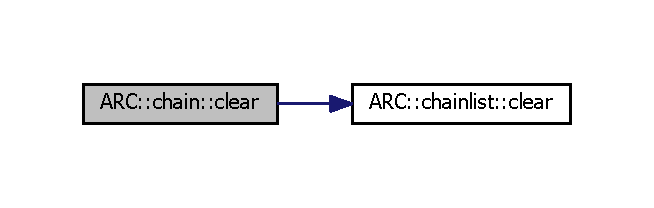
\includegraphics[width=314pt]{classARC_1_1chain_a61d47f9599d4f7176b8870f825305011_cgraph}
\end{center}
\end{figure}
\hypertarget{classARC_1_1chain_a6b7202e64c0a4f5d4f3f8a31f9d27e20}{}\label{classARC_1_1chain_a6b7202e64c0a4f5d4f3f8a31f9d27e20} 
\index{A\+R\+C\+::chain@{A\+R\+C\+::chain}!dump@{dump}}
\index{dump@{dump}!A\+R\+C\+::chain@{A\+R\+C\+::chain}}
\subsubsection{\texorpdfstring{dump()}{dump()}}
{\footnotesize\ttfamily template$<$class particle, class int\+\_\+par$>$ \\
void \hyperlink{classARC_1_1chain}{A\+R\+C\+::chain}$<$ particle, int\+\_\+par $>$\+::dump (\begin{DoxyParamCaption}\item[{const char $\ast$}]{filename }\end{DoxyParamCaption})\hspace{0.3cm}{\ttfamily [inline]}}



Data Dumping to file function. 

Dump chain data into file (binary format) using fwrite. The first variable in the dumping data is particle number \#num The second is the particle chain list index array \#list The third is one dimensional array data storing \#t, \#B, \#w, \#X, \#V generated by using \hyperlink{classARC_1_1chain_ad098493cd057ac19786f5bc85f9ab25d}{backup()}. The forth is center of mass particle data The fifth is one dimensional array storing the masses of particles 
\begin{DoxyParams}[1]{Parameters}
\mbox{\tt in}  & {\em filename} & file for storing the data \\
\hline
\end{DoxyParams}
Here is the call graph for this function\+:
\nopagebreak
\begin{figure}[H]
\begin{center}
\leavevmode
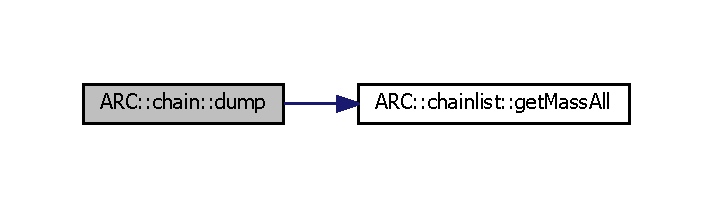
\includegraphics[width=342pt]{classARC_1_1chain_a6b7202e64c0a4f5d4f3f8a31f9d27e20_cgraph}
\end{center}
\end{figure}
\hypertarget{classARC_1_1chain_ae4d0002cceee2397101a43b3755f927e}{}\label{classARC_1_1chain_ae4d0002cceee2397101a43b3755f927e} 
\index{A\+R\+C\+::chain@{A\+R\+C\+::chain}!extrapolation\+\_\+integration@{extrapolation\+\_\+integration}}
\index{extrapolation\+\_\+integration@{extrapolation\+\_\+integration}!A\+R\+C\+::chain@{A\+R\+C\+::chain}}
\subsubsection{\texorpdfstring{extrapolation\+\_\+integration()}{extrapolation\_integration()}}
{\footnotesize\ttfamily template$<$class particle, class int\+\_\+par$>$ \\
double \hyperlink{classARC_1_1chain}{A\+R\+C\+::chain}$<$ particle, int\+\_\+par $>$\+::extrapolation\+\_\+integration (\begin{DoxyParamCaption}\item[{const double}]{ds,  }\item[{const double}]{toff = {\ttfamily -\/1.0},  }\item[{const double3 $\ast$}]{force = {\ttfamily NULL},  }\item[{const bool}]{err\+\_\+ignore = {\ttfamily false} }\end{DoxyParamCaption})\hspace{0.3cm}{\ttfamily [inline]}}



Extrapolation integration. 

Use extrapolation method to get highly accurate integration based on \hyperlink{classARC_1_1chain_aff3cd92c840d1bbbc903a8a07eb079d0}{Leapfrog\+\_\+step\+\_\+forward()}. The auto-\/determination of extrapolation orders based on the accuracy requirement is used.


\begin{DoxyParams}[1]{Parameters}
\mbox{\tt in}  & {\em ds} & integration step size \\
\hline
\mbox{\tt in}  & {\em toff} & ending physical time
\begin{DoxyItemize}
\item if value is negative, it means integration will be done with fixed step size {\itshape ds} 
\item if value is positive and after step {\itshape ds}, the ending physical time is larger than {\itshape toff}, the interpolation of physical time \#t (dense output) will be done instead of integration. In this case, the data are kept as initial values. Instead, the returning value is the ds modification factor (negative value), which can be used to modified current {\itshape ds} and redo the integration by calling this function again with new ds to approach ending physical time of {\itshape toff}. Notice if the required time sychronization criterion (set in chainpars.\+set\+E\+X\+P()) is small ($<$phase and energy error criterion), several iteration may be needed to get the physical time below this criterion. 
\end{DoxyItemize}\\
\hline
\mbox{\tt in}  & {\em force} & external force (not perturber forces which are calculated in pert\+\_\+force) \\
\hline
\mbox{\tt in}  & {\em err\+\_\+ignore} & if true, force integration and ignore error criterion (default false) \\
\hline
\end{DoxyParams}
\begin{DoxyReturn}{Returns}
factor
\begin{DoxyItemize}
\item if factor is positive, it is optimized step size modification factor for next step ({\itshape ds} $\ast$= factor)
\item if factor is negative and {\itshape toff$>$0}; the -\/factor is used for calculate new ds\textquotesingle{} = -\/factor $\ast$ {\itshape ds}. Thus this function should be called again with new step size ds\textquotesingle{} and the new result should have ending physical time close to {\itshape toff}.
\item if factor is zero, maximum extrapolation sequence index (accuracy order/iteration times) is fixed (\hyperlink{classARC_1_1chainpars}{A\+R\+C\+::chainpars}) and err\+\_\+ingore is false, it means the error criterion cannot be satisfied with current maximum sequence index. In this case no integration is done and the data are kept as initial values. User should reduce the integration step and re-\/call this function. 
\end{DoxyItemize}
\end{DoxyReturn}
Here is the call graph for this function\+:
\nopagebreak
\begin{figure}[H]
\begin{center}
\leavevmode
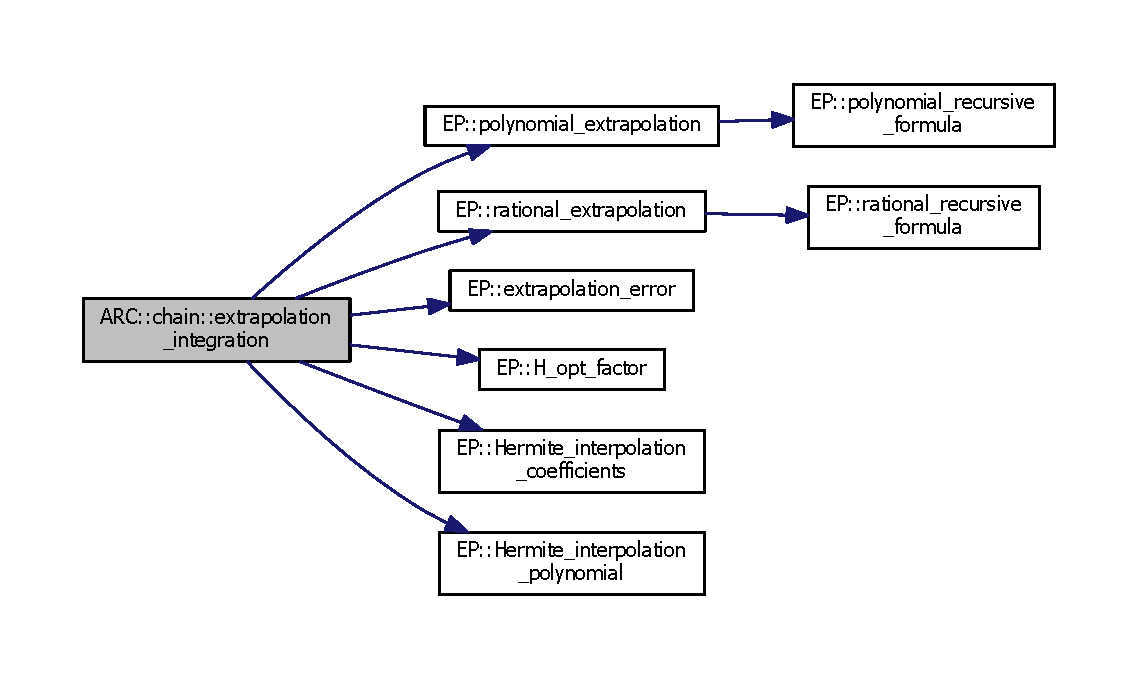
\includegraphics[width=350pt]{classARC_1_1chain_ae4d0002cceee2397101a43b3755f927e_cgraph}
\end{center}
\end{figure}
\hypertarget{classARC_1_1chain_a0c0cadba6cebb17e4d55b40ac98a608a}{}\label{classARC_1_1chain_a0c0cadba6cebb17e4d55b40ac98a608a} 
\index{A\+R\+C\+::chain@{A\+R\+C\+::chain}!find\+\_\+closest\+\_\+pair@{find\+\_\+closest\+\_\+pair}}
\index{find\+\_\+closest\+\_\+pair@{find\+\_\+closest\+\_\+pair}!A\+R\+C\+::chain@{A\+R\+C\+::chain}}
\subsubsection{\texorpdfstring{find\+\_\+closest\+\_\+pair()}{find\_closest\_pair()}}
{\footnotesize\ttfamily template$<$class particle, class int\+\_\+par$>$ \\
double \hyperlink{classARC_1_1chain}{A\+R\+C\+::chain}$<$ particle, int\+\_\+par $>$\+::find\+\_\+closest\+\_\+pair (\begin{DoxyParamCaption}\item[{int}]{pindex\mbox{[}2\mbox{]} }\end{DoxyParamCaption})\hspace{0.3cm}{\ttfamily [inline]}}



Find the closest pair. 

Find the closest pair using relative positions 
\begin{DoxyParams}[1]{Parameters}
\mbox{\tt in}  & {\em pindex} & two element array used for storing pair index. \\
\hline
\end{DoxyParams}
\begin{DoxyReturn}{Returns}
the relative distance of this pair 
\end{DoxyReturn}
\hypertarget{classARC_1_1chain_a7e4f81985bb88e0fb0fcc739b9790396}{}\label{classARC_1_1chain_a7e4f81985bb88e0fb0fcc739b9790396} 
\index{A\+R\+C\+::chain@{A\+R\+C\+::chain}!find\+\_\+strong\+\_\+pair@{find\+\_\+strong\+\_\+pair}}
\index{find\+\_\+strong\+\_\+pair@{find\+\_\+strong\+\_\+pair}!A\+R\+C\+::chain@{A\+R\+C\+::chain}}
\subsubsection{\texorpdfstring{find\+\_\+strong\+\_\+pair()}{find\_strong\_pair()}}
{\footnotesize\ttfamily template$<$class particle, class int\+\_\+par$>$ \\
double \hyperlink{classARC_1_1chain}{A\+R\+C\+::chain}$<$ particle, int\+\_\+par $>$\+::find\+\_\+strong\+\_\+pair (\begin{DoxyParamCaption}\item[{int}]{pindex\mbox{[}2\mbox{]} }\end{DoxyParamCaption})\hspace{0.3cm}{\ttfamily [inline]}}



Find the most strongly interacted pair. 

Find the most strongly interacted pair. First the dacc\mbox{[}i\mbox{]} = acc\mbox{[}i+1\mbox{]}-\/acc\mbox{[}i\mbox{]} (i=0, num-\/1) is calculated, then select the maximum dacc\mbox{[}i\mbox{]}, the corresponding two particles are selected as the strong pair. Their indice are written to pindex. 
\begin{DoxyParams}[1]{Parameters}
\mbox{\tt in}  & {\em pindex} & two element array used for storing pair index. \\
\hline
\end{DoxyParams}
\begin{DoxyReturn}{Returns}
the acceleraction difference of this pair 
\end{DoxyReturn}
\hypertarget{classARC_1_1chain_af9bdf54999606c0d6f32843f0d53d8c4}{}\label{classARC_1_1chain_af9bdf54999606c0d6f32843f0d53d8c4} 
\index{A\+R\+C\+::chain@{A\+R\+C\+::chain}!get\+\_\+int\+\_\+par@{get\+\_\+int\+\_\+par}}
\index{get\+\_\+int\+\_\+par@{get\+\_\+int\+\_\+par}!A\+R\+C\+::chain@{A\+R\+C\+::chain}}
\subsubsection{\texorpdfstring{get\+\_\+int\+\_\+par()}{get\_int\_par()}}
{\footnotesize\ttfamily template$<$class particle, class int\+\_\+par$>$ \\
int\+\_\+par\& \hyperlink{classARC_1_1chain}{A\+R\+C\+::chain}$<$ particle, int\+\_\+par $>$\+::get\+\_\+int\+\_\+par (\begin{DoxyParamCaption}{ }\end{DoxyParamCaption})\hspace{0.3cm}{\ttfamily [inline]}}



Get interaction parameter. 

\begin{DoxyReturn}{Returns}
The reference of Int\+\_\+pars, can be modified 
\end{DoxyReturn}
\hypertarget{classARC_1_1chain_aec4fe3207a5fe2d0a254bdd4bb54ae7f}{}\label{classARC_1_1chain_aec4fe3207a5fe2d0a254bdd4bb54ae7f} 
\index{A\+R\+C\+::chain@{A\+R\+C\+::chain}!get\+Ekin@{get\+Ekin}}
\index{get\+Ekin@{get\+Ekin}!A\+R\+C\+::chain@{A\+R\+C\+::chain}}
\subsubsection{\texorpdfstring{get\+Ekin()}{getEkin()}}
{\footnotesize\ttfamily template$<$class particle, class int\+\_\+par$>$ \\
double \hyperlink{classARC_1_1chain}{A\+R\+C\+::chain}$<$ particle, int\+\_\+par $>$\+::get\+Ekin (\begin{DoxyParamCaption}{ }\end{DoxyParamCaption}) const\hspace{0.3cm}{\ttfamily [inline]}}



Get current kinetic energy. 

\begin{DoxyReturn}{Returns}
current kinetic energy 
\end{DoxyReturn}
\hypertarget{classARC_1_1chain_a5e5a7da2a07800be47623794fe6fe44d}{}\label{classARC_1_1chain_a5e5a7da2a07800be47623794fe6fe44d} 
\index{A\+R\+C\+::chain@{A\+R\+C\+::chain}!get\+List@{get\+List}}
\index{get\+List@{get\+List}!A\+R\+C\+::chain@{A\+R\+C\+::chain}}
\subsubsection{\texorpdfstring{get\+List()}{getList()}}
{\footnotesize\ttfamily template$<$class particle, class int\+\_\+par$>$ \\
void \hyperlink{classARC_1_1chain}{A\+R\+C\+::chain}$<$ particle, int\+\_\+par $>$\+::get\+List (\begin{DoxyParamCaption}\item[{std\+::size\+\_\+t $\ast$}]{indexlist }\end{DoxyParamCaption})\hspace{0.3cm}{\ttfamily [inline]}}



Get chain list. 

Obtain the chain list index ordered by the nearest distances of particles. 
\begin{DoxyParams}[1]{Parameters}
\mbox{\tt out}  & {\em indexlist} & integer array to store the chain list (size of num) \\
\hline
\end{DoxyParams}
\hypertarget{classARC_1_1chain_a582ad9ae8003400e06bba908d70d60d9}{}\label{classARC_1_1chain_a582ad9ae8003400e06bba908d70d60d9} 
\index{A\+R\+C\+::chain@{A\+R\+C\+::chain}!getN@{getN}}
\index{getN@{getN}!A\+R\+C\+::chain@{A\+R\+C\+::chain}}
\subsubsection{\texorpdfstring{get\+N()}{getN()}}
{\footnotesize\ttfamily template$<$class particle, class int\+\_\+par$>$ \\
const int \hyperlink{classARC_1_1chain}{A\+R\+C\+::chain}$<$ particle, int\+\_\+par $>$\+::getN (\begin{DoxyParamCaption}{ }\end{DoxyParamCaption}) const\hspace{0.3cm}{\ttfamily [inline]}}



Get current number of chain members. 

Notice this is not always the number of particles. If Add\+P(), \hyperlink{classARC_1_1chain_a450a7459b076331b6aaa888d209e888c}{remove\+P()} are used, \hyperlink{classARC_1_1chain_a3fe37720ceb48c14905c92d3e25e71a4}{init()} should be called first to get consistent number. \begin{DoxyReturn}{Returns}
\+: number of chain members 
\end{DoxyReturn}
\hypertarget{classARC_1_1chain_ad8bacf5ad6ea0bb31bdb457e4c626701}{}\label{classARC_1_1chain_ad8bacf5ad6ea0bb31bdb457e4c626701} 
\index{A\+R\+C\+::chain@{A\+R\+C\+::chain}!getP@{getP}}
\index{getP@{getP}!A\+R\+C\+::chain@{A\+R\+C\+::chain}}
\subsubsection{\texorpdfstring{get\+P()}{getP()}}
{\footnotesize\ttfamily template$<$class particle, class int\+\_\+par$>$ \\
const particle\& \hyperlink{classARC_1_1chain}{A\+R\+C\+::chain}$<$ particle, int\+\_\+par $>$\+::getP (\begin{DoxyParamCaption}\item[{const std\+::size\+\_\+t}]{i }\end{DoxyParamCaption}) const\hspace{0.3cm}{\ttfamily [inline]}}



Get particle i (const reference) 

\begin{DoxyReturn}{Returns}
\+: particle i (const reference) 
\end{DoxyReturn}
\hypertarget{classARC_1_1chain_a992795e009faf43b59fc338350ae210c}{}\label{classARC_1_1chain_a992795e009faf43b59fc338350ae210c} 
\index{A\+R\+C\+::chain@{A\+R\+C\+::chain}!get\+Pext@{get\+Pext}}
\index{get\+Pext@{get\+Pext}!A\+R\+C\+::chain@{A\+R\+C\+::chain}}
\subsubsection{\texorpdfstring{get\+Pext()}{getPext()}}
{\footnotesize\ttfamily template$<$class particle, class int\+\_\+par$>$ \\
const particle\& \hyperlink{classARC_1_1chain}{A\+R\+C\+::chain}$<$ particle, int\+\_\+par $>$\+::get\+Pext (\begin{DoxyParamCaption}\item[{const std\+::size\+\_\+t}]{i }\end{DoxyParamCaption}) const\hspace{0.3cm}{\ttfamily [inline]}}



Get pertuber particle i (const reference) 

\begin{DoxyReturn}{Returns}
\+: pertuber particle i (const reference) 
\end{DoxyReturn}
\hypertarget{classARC_1_1chain_ade5db39891ff7a2d10ac38786ab866c1}{}\label{classARC_1_1chain_ade5db39891ff7a2d10ac38786ab866c1} 
\index{A\+R\+C\+::chain@{A\+R\+C\+::chain}!get\+Pot@{get\+Pot}}
\index{get\+Pot@{get\+Pot}!A\+R\+C\+::chain@{A\+R\+C\+::chain}}
\subsubsection{\texorpdfstring{get\+Pot()}{getPot()}}
{\footnotesize\ttfamily template$<$class particle, class int\+\_\+par$>$ \\
double \hyperlink{classARC_1_1chain}{A\+R\+C\+::chain}$<$ particle, int\+\_\+par $>$\+::get\+Pot (\begin{DoxyParamCaption}{ }\end{DoxyParamCaption}) const\hspace{0.3cm}{\ttfamily [inline]}}



Get current potential energy. 

\begin{DoxyReturn}{Returns}
current potetnial energy (negative value for bounded systems) 
\end{DoxyReturn}
\hypertarget{classARC_1_1chain_a1404204bd5665aa2d12d57cf653b779c}{}\label{classARC_1_1chain_a1404204bd5665aa2d12d57cf653b779c} 
\index{A\+R\+C\+::chain@{A\+R\+C\+::chain}!get\+Pt@{get\+Pt}}
\index{get\+Pt@{get\+Pt}!A\+R\+C\+::chain@{A\+R\+C\+::chain}}
\subsubsection{\texorpdfstring{get\+Pt()}{getPt()}}
{\footnotesize\ttfamily template$<$class particle, class int\+\_\+par$>$ \\
double \hyperlink{classARC_1_1chain}{A\+R\+C\+::chain}$<$ particle, int\+\_\+par $>$\+::get\+Pt (\begin{DoxyParamCaption}{ }\end{DoxyParamCaption}) const\hspace{0.3cm}{\ttfamily [inline]}}



Get current time momemtum $Pt$ (current system binding energy) 

\begin{DoxyReturn}{Returns}
time momemtum $Pt$ (current system binding energy $(-H(t))$) 
\end{DoxyReturn}
\hypertarget{classARC_1_1chain_ad21bc515c01cf62e65d6d749d8babd63}{}\label{classARC_1_1chain_ad21bc515c01cf62e65d6d749d8babd63} 
\index{A\+R\+C\+::chain@{A\+R\+C\+::chain}!get\+Time@{get\+Time}}
\index{get\+Time@{get\+Time}!A\+R\+C\+::chain@{A\+R\+C\+::chain}}
\subsubsection{\texorpdfstring{get\+Time()}{getTime()}}
{\footnotesize\ttfamily template$<$class particle, class int\+\_\+par$>$ \\
double \hyperlink{classARC_1_1chain}{A\+R\+C\+::chain}$<$ particle, int\+\_\+par $>$\+::get\+Time (\begin{DoxyParamCaption}{ }\end{DoxyParamCaption}) const\hspace{0.3cm}{\ttfamily [inline]}}



Get current physical time. 

\begin{DoxyReturn}{Returns}
current physical time 
\end{DoxyReturn}
\hypertarget{classARC_1_1chain_abdd62eb43e4a7b5eca10190c90ed190f}{}\label{classARC_1_1chain_abdd62eb43e4a7b5eca10190c90ed190f} 
\index{A\+R\+C\+::chain@{A\+R\+C\+::chain}!getw@{getw}}
\index{getw@{getw}!A\+R\+C\+::chain@{A\+R\+C\+::chain}}
\subsubsection{\texorpdfstring{getw()}{getw()}}
{\footnotesize\ttfamily template$<$class particle, class int\+\_\+par$>$ \\
double \hyperlink{classARC_1_1chain}{A\+R\+C\+::chain}$<$ particle, int\+\_\+par $>$\+::getw (\begin{DoxyParamCaption}{ }\end{DoxyParamCaption}) const\hspace{0.3cm}{\ttfamily [inline]}}



Get current integrated time transformation function value $w$. 

$w$\+: $ \frac{dw}{dt} = \sum_k \frac{\partial W}{\partial \vec{r_k}} \bullet \vec{v_k} $ (see W in \hyperlink{classARC_1_1chain_abcfc20c1694a1d68a324ea9a08863af3}{get\+W()};) \begin{DoxyReturn}{Returns}
$w$ 
\end{DoxyReturn}
\hypertarget{classARC_1_1chain_abcfc20c1694a1d68a324ea9a08863af3}{}\label{classARC_1_1chain_abcfc20c1694a1d68a324ea9a08863af3} 
\index{A\+R\+C\+::chain@{A\+R\+C\+::chain}!getW@{getW}}
\index{getW@{getW}!A\+R\+C\+::chain@{A\+R\+C\+::chain}}
\subsubsection{\texorpdfstring{get\+W()}{getW()}}
{\footnotesize\ttfamily template$<$class particle, class int\+\_\+par$>$ \\
double \hyperlink{classARC_1_1chain}{A\+R\+C\+::chain}$<$ particle, int\+\_\+par $>$\+::getW (\begin{DoxyParamCaption}{ }\end{DoxyParamCaption}) const\hspace{0.3cm}{\ttfamily [inline]}}



Get current time transformation function value $W$. 

The $W$ is defined in \+::\+A\+R\+C\+::pair\+\_\+\+A\+W(). \begin{DoxyReturn}{Returns}
$W$ 
\end{DoxyReturn}
\hypertarget{classARC_1_1chain_a3fe37720ceb48c14905c92d3e25e71a4}{}\label{classARC_1_1chain_a3fe37720ceb48c14905c92d3e25e71a4} 
\index{A\+R\+C\+::chain@{A\+R\+C\+::chain}!init@{init}}
\index{init@{init}!A\+R\+C\+::chain@{A\+R\+C\+::chain}}
\subsubsection{\texorpdfstring{init()}{init()}}
{\footnotesize\ttfamily template$<$class particle, class int\+\_\+par$>$ \\
void \hyperlink{classARC_1_1chain}{A\+R\+C\+::chain}$<$ particle, int\+\_\+par $>$\+::init (\begin{DoxyParamCaption}\item[{const double}]{time }\end{DoxyParamCaption})\hspace{0.3cm}{\ttfamily [inline]}}



Initialization. 

Initialize chain based on particle list \#p. After this function, positions and velocities of particles in \#p will be shifted to their center-\/of-\/mass frame. ~\newline
 Chain order list \#list, relative position \#X, velocity \#V, initial system energy \#\+Pt and initial time transformation parameter \#w are calculated. The particle modification indicator (\hyperlink{classARC_1_1chain_a29ff9707fe94a554966c885d9bafa819}{is\+Pmod()}) will be set to false. 
\begin{DoxyParams}[1]{Parameters}
\mbox{\tt in}  & {\em time} & current time of particle system \\
\hline
\end{DoxyParams}
Here is the call graph for this function\+:
\nopagebreak
\begin{figure}[H]
\begin{center}
\leavevmode
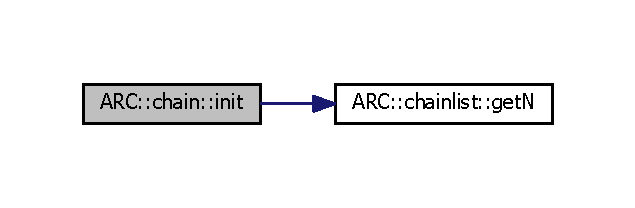
\includegraphics[width=305pt]{classARC_1_1chain_a3fe37720ceb48c14905c92d3e25e71a4_cgraph}
\end{center}
\end{figure}
\hypertarget{classARC_1_1chain_a1c6de84a911feff1425dfb59e7a89087}{}\label{classARC_1_1chain_a1c6de84a911feff1425dfb59e7a89087} 
\index{A\+R\+C\+::chain@{A\+R\+C\+::chain}!init\+Pext@{init\+Pext}}
\index{init\+Pext@{init\+Pext}!A\+R\+C\+::chain@{A\+R\+C\+::chain}}
\subsubsection{\texorpdfstring{init\+Pext()}{initPext()}}
{\footnotesize\ttfamily template$<$class particle, class int\+\_\+par$>$ \\
void \hyperlink{classARC_1_1chain}{A\+R\+C\+::chain}$<$ particle, int\+\_\+par $>$\+::init\+Pext (\begin{DoxyParamCaption}\item[{const std\+::size\+\_\+t}]{n }\end{DoxyParamCaption})\hspace{0.3cm}{\ttfamily [inline]}}



Allocate memory for perturber list. 

Allocate memory for perturber particle list with maximum number of {\itshape n} 
\begin{DoxyParams}[1]{Parameters}
\mbox{\tt in}  & {\em n} & maximum number of perturbers \\
\hline
\end{DoxyParams}
Here is the call graph for this function\+:
\nopagebreak
\begin{figure}[H]
\begin{center}
\leavevmode
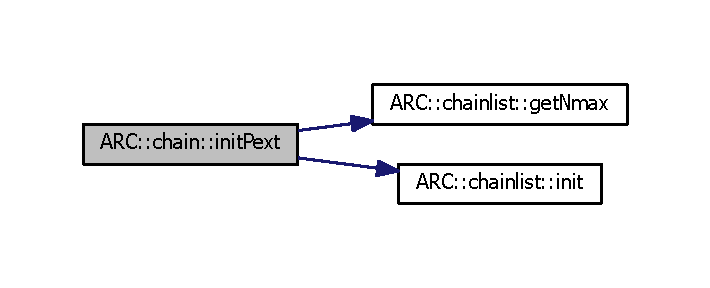
\includegraphics[width=341pt]{classARC_1_1chain_a1c6de84a911feff1425dfb59e7a89087_cgraph}
\end{center}
\end{figure}
\hypertarget{classARC_1_1chain_a29ff9707fe94a554966c885d9bafa819}{}\label{classARC_1_1chain_a29ff9707fe94a554966c885d9bafa819} 
\index{A\+R\+C\+::chain@{A\+R\+C\+::chain}!is\+Pmod@{is\+Pmod}}
\index{is\+Pmod@{is\+Pmod}!A\+R\+C\+::chain@{A\+R\+C\+::chain}}
\subsubsection{\texorpdfstring{is\+Pmod()}{isPmod()}}
{\footnotesize\ttfamily template$<$class particle, class int\+\_\+par$>$ \\
bool \hyperlink{classARC_1_1chain}{A\+R\+C\+::chain}$<$ particle, int\+\_\+par $>$\+::is\+Pmod (\begin{DoxyParamCaption}{ }\end{DoxyParamCaption}) const\hspace{0.3cm}{\ttfamily [inline]}}



Indicator of changes in particle list \#p. 

Reture true if particle list is modifed, in this case, the chain may need to be initialized again \begin{DoxyReturn}{Returns}
true\+: \hyperlink{classParticle}{Particle} list is modified 
\end{DoxyReturn}
\hypertarget{classARC_1_1chain_a7de218a1874b150ee44a05aa9d7b7b6d}{}\label{classARC_1_1chain_a7de218a1874b150ee44a05aa9d7b7b6d} 
\index{A\+R\+C\+::chain@{A\+R\+C\+::chain}!is\+Porigin@{is\+Porigin}}
\index{is\+Porigin@{is\+Porigin}!A\+R\+C\+::chain@{A\+R\+C\+::chain}}
\subsubsection{\texorpdfstring{is\+Porigin()}{isPorigin()}}
{\footnotesize\ttfamily template$<$class particle, class int\+\_\+par$>$ \\
int \hyperlink{classARC_1_1chain}{A\+R\+C\+::chain}$<$ particle, int\+\_\+par $>$\+::is\+Porigin (\begin{DoxyParamCaption}{ }\end{DoxyParamCaption}) const\hspace{0.3cm}{\ttfamily [inline]}}



Indicator of particle frame. 

Return true if particles positions and velocities in \#p are in original frame \begin{DoxyReturn}{Returns}
\+: -\/ 1\+: In the original frame
\begin{DoxyItemize}
\item 2\+: Only positions are in the original frame
\item 0\+: In the center-\/of-\/mass frame 
\end{DoxyItemize}
\end{DoxyReturn}
Here is the caller graph for this function\+:
\nopagebreak
\begin{figure}[H]
\begin{center}
\leavevmode
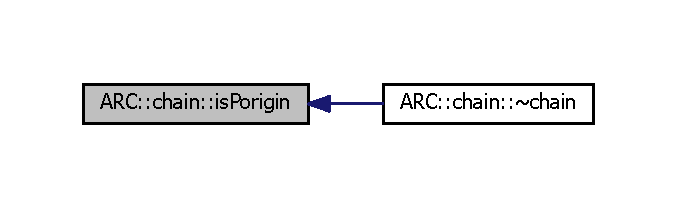
\includegraphics[width=325pt]{classARC_1_1chain_a7de218a1874b150ee44a05aa9d7b7b6d_icgraph}
\end{center}
\end{figure}
\hypertarget{classARC_1_1chain_aff3cd92c840d1bbbc903a8a07eb079d0}{}\label{classARC_1_1chain_aff3cd92c840d1bbbc903a8a07eb079d0} 
\index{A\+R\+C\+::chain@{A\+R\+C\+::chain}!Leapfrog\+\_\+step\+\_\+forward@{Leapfrog\+\_\+step\+\_\+forward}}
\index{Leapfrog\+\_\+step\+\_\+forward@{Leapfrog\+\_\+step\+\_\+forward}!A\+R\+C\+::chain@{A\+R\+C\+::chain}}
\subsubsection{\texorpdfstring{Leapfrog\+\_\+step\+\_\+forward()}{Leapfrog\_step\_forward()}}
{\footnotesize\ttfamily template$<$class particle, class int\+\_\+par$>$ \\
void \hyperlink{classARC_1_1chain}{A\+R\+C\+::chain}$<$ particle, int\+\_\+par $>$\+::Leapfrog\+\_\+step\+\_\+forward (\begin{DoxyParamCaption}\item[{const double}]{s,  }\item[{const int}]{n,  }\item[{const double3 $\ast$}]{force = {\ttfamily NULL},  }\item[{int}]{check\+\_\+flag = {\ttfamily 1},  }\item[{double $\ast$$\ast$}]{dpoly = {\ttfamily NULL},  }\item[{const int}]{ndmax = {\ttfamily 0} }\end{DoxyParamCaption})\hspace{0.3cm}{\ttfamily [inline]}}



Leapfrog integrator. 

Integration with Leapfrog method. ~\newline
The positions and velocities of particles in \#p will be integrated in the center-\/of-\/mass frame 
\begin{DoxyParams}[1]{Parameters}
\mbox{\tt in}  & {\em s} & Integration step size \\
\hline
\mbox{\tt in}  & {\em n} & number of sub-\/steps needed to be divided. Integration step size is ({\itshape s/{\itshape n})} and do {\itshape n} times as\+: X(s/2n)V(s/n)X(s/n)V(s/n)..X(s/2n) \\
\hline
\mbox{\tt in}  & {\em force} & external force (not perturber forces which are calculated in pert\+\_\+force) \\
\hline
\mbox{\tt in}  & {\em check\+\_\+flag} & 2\+: check link every step; 1\+: check link at then end; 0 \+:no check \\
\hline
\mbox{\tt in}  & {\em dpoly} & two dimensional array for storing 0 to {\itshape }(ndmax-\/$\ast$)\textquotesingle{}th order central difference of physical time \#t at {\itshape s/2} as a function of {\itshape s}, array size should be \mbox{[}ndmax\mbox{]}\mbox{[}1\mbox{]} \\
\hline
\mbox{\tt in}  & {\em ndmax} & dpoly array size and the maximum difference is ndmax-\/$\ast$ \\
\hline
\end{DoxyParams}
Here is the call graph for this function\+:
\nopagebreak
\begin{figure}[H]
\begin{center}
\leavevmode
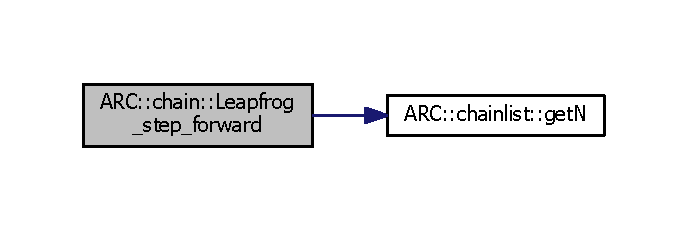
\includegraphics[width=330pt]{classARC_1_1chain_aff3cd92c840d1bbbc903a8a07eb079d0_cgraph}
\end{center}
\end{figure}
\hypertarget{classARC_1_1chain_a34cb0bde571c3d8cc8204c3e7c11a821}{}\label{classARC_1_1chain_a34cb0bde571c3d8cc8204c3e7c11a821} 
\index{A\+R\+C\+::chain@{A\+R\+C\+::chain}!link\+\_\+int\+\_\+par@{link\+\_\+int\+\_\+par}}
\index{link\+\_\+int\+\_\+par@{link\+\_\+int\+\_\+par}!A\+R\+C\+::chain@{A\+R\+C\+::chain}}
\subsubsection{\texorpdfstring{link\+\_\+int\+\_\+par()}{link\_int\_par()}}
{\footnotesize\ttfamily template$<$class particle, class int\+\_\+par$>$ \\
void \hyperlink{classARC_1_1chain}{A\+R\+C\+::chain}$<$ particle, int\+\_\+par $>$\+::link\+\_\+int\+\_\+par (\begin{DoxyParamCaption}\item[{int\+\_\+par \&}]{par }\end{DoxyParamCaption})\hspace{0.3cm}{\ttfamily [inline]}}



link interaction parameter class 

link interaction parameter clsss to chain for the acceleration calculation functions 
\begin{DoxyParams}[1]{Parameters}
\mbox{\tt in}  & {\em par} & int\+\_\+par type interaction parameter class. The address will be stored (not copy) \\
\hline
\end{DoxyParams}
\hypertarget{classARC_1_1chain_a921a250cfcfe7a5b8e597ddcb03730ec}{}\label{classARC_1_1chain_a921a250cfcfe7a5b8e597ddcb03730ec} 
\index{A\+R\+C\+::chain@{A\+R\+C\+::chain}!load@{load}}
\index{load@{load}!A\+R\+C\+::chain@{A\+R\+C\+::chain}}
\subsubsection{\texorpdfstring{load()}{load()}}
{\footnotesize\ttfamily template$<$class particle, class int\+\_\+par$>$ \\
void \hyperlink{classARC_1_1chain}{A\+R\+C\+::chain}$<$ particle, int\+\_\+par $>$\+::load (\begin{DoxyParamCaption}\item[{const char $\ast$}]{filename }\end{DoxyParamCaption})\hspace{0.3cm}{\ttfamily [inline]}}



Data reading from file function. 

Read chain data from binary file generated by \hyperlink{classARC_1_1chain_a6b7202e64c0a4f5d4f3f8a31f9d27e20}{dump()}. The first variable in the dumping data is particle number \#num The second is the particle chain list index array \#list The third is one dimensional array data storing \#t, \#B, \#w, \#X, \#V generated by using \hyperlink{classARC_1_1chain_ad098493cd057ac19786f5bc85f9ab25d}{backup()}. The forth is center of mass particle data The fifth is one dimensional array storing the masses of particles

Notice the particle list will allocate new memory to store the particle data. The particle data are in the center-\/of-\/mass frame 
\begin{DoxyParams}[1]{Parameters}
\mbox{\tt in}  & {\em filename} & file for reading the data \\
\hline
\end{DoxyParams}
Here is the call graph for this function\+:
\nopagebreak
\begin{figure}[H]
\begin{center}
\leavevmode
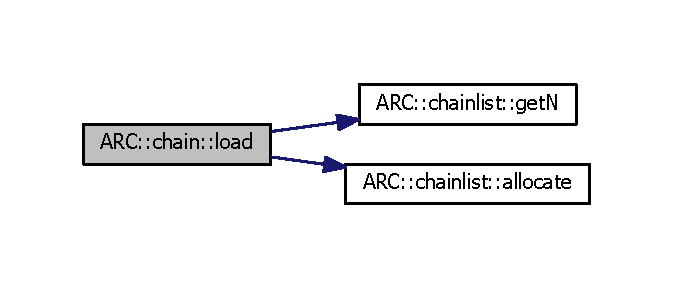
\includegraphics[width=323pt]{classARC_1_1chain_a921a250cfcfe7a5b8e597ddcb03730ec_cgraph}
\end{center}
\end{figure}
\hypertarget{classARC_1_1chain_a4624cf80ecb8804bc08fb7f23fdddb4e}{}\label{classARC_1_1chain_a4624cf80ecb8804bc08fb7f23fdddb4e} 
\index{A\+R\+C\+::chain@{A\+R\+C\+::chain}!print@{print}}
\index{print@{print}!A\+R\+C\+::chain@{A\+R\+C\+::chain}}
\subsubsection{\texorpdfstring{print()}{print()}}
{\footnotesize\ttfamily template$<$class particle, class int\+\_\+par$>$ \\
void \hyperlink{classARC_1_1chain}{A\+R\+C\+::chain}$<$ particle, int\+\_\+par $>$\+::print (\begin{DoxyParamCaption}\item[{std\+::ostream \&}]{fout,  }\item[{const int}]{precision = {\ttfamily 15},  }\item[{const int}]{width = {\ttfamily 15} }\end{DoxyParamCaption})\hspace{0.3cm}{\ttfamily [inline]}}



print chain data 

Print chain data 
\begin{DoxyParams}[1]{Parameters}
\mbox{\tt in}  & {\em fout} & ofstream for printing \\
\hline
\mbox{\tt in}  & {\em precision} & printed precision for one variable \\
\hline
\mbox{\tt in}  & {\em width} & printing width for one variable \\
\hline
\end{DoxyParams}
\hypertarget{classARC_1_1chain_ae14cbd0c85aa090d0848538c6eae0afd}{}\label{classARC_1_1chain_ae14cbd0c85aa090d0848538c6eae0afd} 
\index{A\+R\+C\+::chain@{A\+R\+C\+::chain}!readP@{readP}}
\index{readP@{readP}!A\+R\+C\+::chain@{A\+R\+C\+::chain}}
\subsubsection{\texorpdfstring{read\+P()}{readP()}}
{\footnotesize\ttfamily template$<$class particle, class int\+\_\+par$>$ \\
void \hyperlink{classARC_1_1chain}{A\+R\+C\+::chain}$<$ particle, int\+\_\+par $>$\+::readP (\begin{DoxyParamCaption}\item[{const char $\ast$}]{filename }\end{DoxyParamCaption})\hspace{0.3cm}{\ttfamily [inline]}}



Read particle data from file. 

Read particle data using fread (binary format). Number of particles should be first variable, then the data of particles (the data structure should be consistent with particle class). Notice if read is used, the particle data memory is allocated inside chainlist of chain. 
\begin{DoxyParams}[1]{Parameters}
\mbox{\tt in}  & {\em filename} & file to read the data \\
\hline
\end{DoxyParams}
Here is the call graph for this function\+:
\nopagebreak
\begin{figure}[H]
\begin{center}
\leavevmode
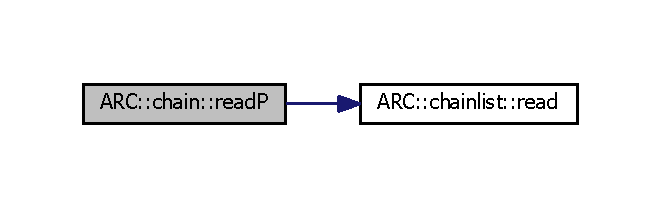
\includegraphics[width=317pt]{classARC_1_1chain_ae14cbd0c85aa090d0848538c6eae0afd_cgraph}
\end{center}
\end{figure}
\hypertarget{classARC_1_1chain_a450a7459b076331b6aaa888d209e888c}{}\label{classARC_1_1chain_a450a7459b076331b6aaa888d209e888c} 
\index{A\+R\+C\+::chain@{A\+R\+C\+::chain}!removeP@{removeP}}
\index{removeP@{removeP}!A\+R\+C\+::chain@{A\+R\+C\+::chain}}
\subsubsection{\texorpdfstring{remove\+P()}{removeP()}}
{\footnotesize\ttfamily template$<$class particle, class int\+\_\+par$>$ \\
void \hyperlink{classARC_1_1chain}{A\+R\+C\+::chain}$<$ particle, int\+\_\+par $>$\+::removeP (\begin{DoxyParamCaption}\item[{const std\+::size\+\_\+t}]{i,  }\item[{bool}]{option = {\ttfamily true} }\end{DoxyParamCaption})\hspace{0.3cm}{\ttfamily [inline]}}



remove one particle 

remove one particle from \#p (see \hyperlink{classARC_1_1chainlist_a16edd790019b6aa7a7f6b5cc3e59a2c3}{A\+R\+C\+::chainlist.\+remove()}) 
\begin{DoxyParams}[1]{Parameters}
\mbox{\tt in}  & {\em i} & particle index in \#p needs to be removed \\
\hline
\mbox{\tt in}  & {\em option} & position update option\+:
\begin{DoxyItemize}
\item true\+: shift last particle to current position (defaulted);
\item false\+: shift all right particle to left by one 
\end{DoxyItemize}\\
\hline
\end{DoxyParams}
Here is the call graph for this function\+:
\nopagebreak
\begin{figure}[H]
\begin{center}
\leavevmode
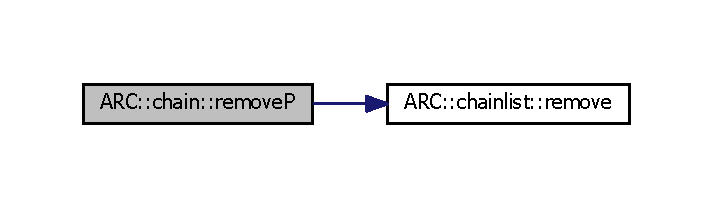
\includegraphics[width=342pt]{classARC_1_1chain_a450a7459b076331b6aaa888d209e888c_cgraph}
\end{center}
\end{figure}
\hypertarget{classARC_1_1chain_a7d563413beb44795b8ecd1348a2d2305}{}\label{classARC_1_1chain_a7d563413beb44795b8ecd1348a2d2305} 
\index{A\+R\+C\+::chain@{A\+R\+C\+::chain}!remove\+Pext@{remove\+Pext}}
\index{remove\+Pext@{remove\+Pext}!A\+R\+C\+::chain@{A\+R\+C\+::chain}}
\subsubsection{\texorpdfstring{remove\+Pext()}{removePext()}}
{\footnotesize\ttfamily template$<$class particle, class int\+\_\+par$>$ \\
void \hyperlink{classARC_1_1chain}{A\+R\+C\+::chain}$<$ particle, int\+\_\+par $>$\+::remove\+Pext (\begin{DoxyParamCaption}\item[{const std\+::size\+\_\+t}]{i,  }\item[{bool}]{option = {\ttfamily true} }\end{DoxyParamCaption})\hspace{0.3cm}{\ttfamily [inline]}}



Remove one perturber. 

Remove one perturber from \#pext 
\begin{DoxyParams}[1]{Parameters}
\mbox{\tt in}  & {\em i} & perturber index in \#pext needs to be removed \\
\hline
\mbox{\tt in}  & {\em option} & position update option\+:
\begin{DoxyItemize}
\item true\+: shift last particle to current position (defaulted);
\item false\+: shift all right particle to left by one 
\end{DoxyItemize}\\
\hline
\end{DoxyParams}
Here is the call graph for this function\+:
\nopagebreak
\begin{figure}[H]
\begin{center}
\leavevmode
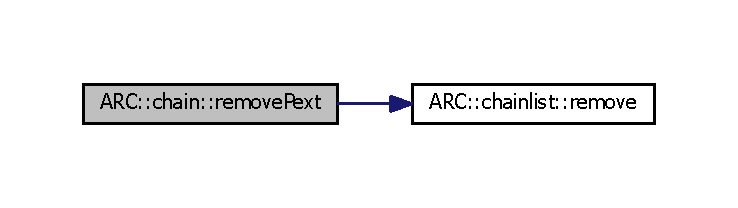
\includegraphics[width=350pt]{classARC_1_1chain_a7d563413beb44795b8ecd1348a2d2305_cgraph}
\end{center}
\end{figure}
\hypertarget{classARC_1_1chain_a5b1bec1324def99667dc6783108d1607}{}\label{classARC_1_1chain_a5b1bec1324def99667dc6783108d1607} 
\index{A\+R\+C\+::chain@{A\+R\+C\+::chain}!restore@{restore}}
\index{restore@{restore}!A\+R\+C\+::chain@{A\+R\+C\+::chain}}
\subsubsection{\texorpdfstring{restore()}{restore()}}
{\footnotesize\ttfamily template$<$class particle, class int\+\_\+par$>$ \\
void \hyperlink{classARC_1_1chain}{A\+R\+C\+::chain}$<$ particle, int\+\_\+par $>$\+::restore (\begin{DoxyParamCaption}\item[{double $\ast$}]{db }\end{DoxyParamCaption})\hspace{0.3cm}{\ttfamily [inline]}}



Restore chain data (\#t, \#\+Pt, \#w, \#X, \#V) 

Restore integration data from one dimensional array, the order of data should be \#t, \#\+Pt, \#w, \#X\mbox{[}\#num\mbox{]}\mbox{[}3\mbox{]}, \#V\mbox{[}\#num\mbox{]}\mbox{[}3\mbox{]}
\begin{DoxyItemize}
\item \#t \+: current physical time
\item \#\+Pt \+: current time momentum (system binding energy)
\item \#w \+: current time transformation parameter
\item \#X \+: current relative position array
\item \#V \+: current relative velocite array 
\begin{DoxyParams}[1]{Parameters}
\mbox{\tt in}  & {\em db} & one dimensional array that storing chain data (array size should be 6$\ast$\#num-\/3) where \#num is the total number of particles in \#p \\
\hline
\end{DoxyParams}

\end{DoxyItemize}

\subsection{Member Data Documentation}
\hypertarget{classARC_1_1chain_a2eead75bd916fa7ffc05341645527847}{}\label{classARC_1_1chain_a2eead75bd916fa7ffc05341645527847} 
\index{A\+R\+C\+::chain@{A\+R\+C\+::chain}!cm@{cm}}
\index{cm@{cm}!A\+R\+C\+::chain@{A\+R\+C\+::chain}}
\subsubsection{\texorpdfstring{cm}{cm}}
{\footnotesize\ttfamily template$<$class particle, class int\+\_\+par$>$ \\
particle \hyperlink{classARC_1_1chain}{A\+R\+C\+::chain}$<$ particle, int\+\_\+par $>$\+::cm}



center mass particle 

\hypertarget{classARC_1_1chain_a7ad20a60e038d16522c11d7fccb47648}{}\label{classARC_1_1chain_a7ad20a60e038d16522c11d7fccb47648} 
\index{A\+R\+C\+::chain@{A\+R\+C\+::chain}!info@{info}}
\index{info@{info}!A\+R\+C\+::chain@{A\+R\+C\+::chain}}
\subsubsection{\texorpdfstring{info}{info}}
{\footnotesize\ttfamily template$<$class particle, class int\+\_\+par$>$ \\
\hyperlink{classARC_1_1chaininfo}{chaininfo}$\ast$ \hyperlink{classARC_1_1chain}{A\+R\+C\+::chain}$<$ particle, int\+\_\+par $>$\+::info}



chain information 



The documentation for this class was generated from the following file\+:\begin{DoxyCompactItemize}
\item 
C\+:/\+Users/longw/\+Documents/\+Git\+Hub/\+A\+R\+C/include/\hyperlink{AR_8h}{A\+R.\+h}\end{DoxyCompactItemize}

\hypertarget{classARC_1_1chaininfo}{}\section{A\+RC\+:\+:chaininfo Class Reference}
\label{classARC_1_1chaininfo}\index{A\+R\+C\+::chaininfo@{A\+R\+C\+::chaininfo}}


class for storing the information of chain (for decision making)  




{\ttfamily \#include $<$A\+R.\+h$>$}

\subsection*{Public Member Functions}
\begin{DoxyCompactItemize}
\item 
\hyperlink{classARC_1_1chaininfo_a9e67e1e081f3a09d8c8bec3b55d108d1}{chaininfo} (const std\+::size\+\_\+t n)
\begin{DoxyCompactList}\small\item\em constructor \end{DoxyCompactList}\item 
void \hyperlink{classARC_1_1chaininfo_ae65957f4d894671dd467a376b898e1a5}{clear} ()
\begin{DoxyCompactList}\small\item\em reset function \end{DoxyCompactList}\item 
\hyperlink{classARC_1_1chaininfo_aca51a64943e31e1ac33473fb90c39a17}{$\sim$chaininfo} ()
\begin{DoxyCompactList}\small\item\em destructor \end{DoxyCompactList}\item 
void \hyperlink{classARC_1_1chaininfo_a75c849e7360a20d88934079a8f5d75f4}{print} (std\+::ostream \&fout, const int precision=10)
\begin{DoxyCompactList}\small\item\em print chain information \end{DoxyCompactList}\item 
void \hyperlink{classARC_1_1chaininfo_a07ad3dcb9540f02984195045357166b0}{Err\+Message} (std\+::ostream \&fout, const int precision=10, const int stat=0, char $\ast$message=N\+U\+LL)
\begin{DoxyCompactList}\small\item\em status message \end{DoxyCompactList}\end{DoxyCompactItemize}
\subsection*{Public Attributes}
\begin{DoxyCompactItemize}
\item 
int \hyperlink{classARC_1_1chaininfo_a64ae72bf5fd209d92b95393826f2a358}{status}
\begin{DoxyCompactList}\small\item\em current status of integration \end{DoxyCompactList}\item 
int \hyperlink{classARC_1_1chaininfo_a0bd3d3a4b97bba8fa1baea9f077f30a7}{intcount}
\begin{DoxyCompactList}\small\item\em current extrapolation sequence index when an accident happen \end{DoxyCompactList}\item 
int \hyperlink{classARC_1_1chaininfo_ab043612acf18c1c850737f67bcb6e141}{inti}
\begin{DoxyCompactList}\small\item\em current number of substeps \end{DoxyCompactList}\item 
int \hyperlink{classARC_1_1chaininfo_a50deb77aefe8f664d65f7320098d4726}{i1}
\item 
int \hyperlink{classARC_1_1chaininfo_a60f94a1f01c83934ad975f5d82638ef1}{i2}
\begin{DoxyCompactList}\small\item\em index of particles causing the accident \end{DoxyCompactList}\item 
int \hyperlink{classARC_1_1chaininfo_a4c85d251b74ed69a458e1b33b9f1173c}{num}
\begin{DoxyCompactList}\small\item\em number of particles \end{DoxyCompactList}\item 
double \hyperlink{classARC_1_1chaininfo_af689a2456268b30374ae6046704511f0}{ds}
\item 
double \hyperlink{classARC_1_1chaininfo_a3185aadb946f5d958016a35f40d0341f}{subds}
\item 
double \hyperlink{classARC_1_1chaininfo_a470e18cf65e805ff41ea3098da9cdd10}{subdt}
\begin{DoxyCompactList}\small\item\em step size, substep size, substep corresponding time step \end{DoxyCompactList}\item 
double \hyperlink{classARC_1_1chaininfo_a4c24552fe5d2005171233432f3cf3832}{toff}
\begin{DoxyCompactList}\small\item\em physical ending time \end{DoxyCompactList}\item 
double \hyperlink{classARC_1_1chaininfo_a83dc2c6904ccf789ac299db95fa57bc5}{perr}
\item 
double \hyperlink{classARC_1_1chaininfo_aa5687aa0deb33f878f2283befe978d5f}{perr0}
\begin{DoxyCompactList}\small\item\em phase error (current and previous) \end{DoxyCompactList}\item 
double \hyperlink{classARC_1_1chaininfo_a2a4787b1089da59e9ad8f008d211faed}{eerr}
\item 
double \hyperlink{classARC_1_1chaininfo_aa25da11049199a727d6d94c172ed93ae}{eerr0}
\begin{DoxyCompactList}\small\item\em energy error (current and previous) \end{DoxyCompactList}\item 
double \hyperlink{classARC_1_1chaininfo_a7732d57314ddb49eb996eb41056a0140}{Ekin}
\item 
double \hyperlink{classARC_1_1chaininfo_afcefd59678495b4fb0e42b5b481cd875}{Pot}
\item 
double \hyperlink{classARC_1_1chaininfo_a1072512674fc88001d6cd560a6c7d295}{W}
\begin{DoxyCompactList}\small\item\em kinetic energy, potential energy and time transformation function \end{DoxyCompactList}\item 
double \hyperlink{classARC_1_1chaininfo_a665c9bc8dfdac9fdee4947e8aaffd8c6}{terr}
\begin{DoxyCompactList}\small\item\em time error \end{DoxyCompactList}\item 
double $\ast$ \hyperlink{classARC_1_1chaininfo_aee6f50a67bbc6f5ed555faa6fe2ecf51}{data}
\begin{DoxyCompactList}\small\item\em chain data for backuping \end{DoxyCompactList}\end{DoxyCompactItemize}


\subsection{Detailed Description}
class for storing the information of chain (for decision making) 

It is used to store the information when an accident happen with chain.\+status != 0. 

\subsection{Constructor \& Destructor Documentation}
\hypertarget{classARC_1_1chaininfo_a9e67e1e081f3a09d8c8bec3b55d108d1}{}\label{classARC_1_1chaininfo_a9e67e1e081f3a09d8c8bec3b55d108d1} 
\index{A\+R\+C\+::chaininfo@{A\+R\+C\+::chaininfo}!chaininfo@{chaininfo}}
\index{chaininfo@{chaininfo}!A\+R\+C\+::chaininfo@{A\+R\+C\+::chaininfo}}
\subsubsection{\texorpdfstring{chaininfo()}{chaininfo()}}
{\footnotesize\ttfamily A\+R\+C\+::chaininfo\+::chaininfo (\begin{DoxyParamCaption}\item[{const std\+::size\+\_\+t}]{n }\end{DoxyParamCaption})\hspace{0.3cm}{\ttfamily [inline]}}



constructor 

Set all variables to infinity 
\begin{DoxyParams}[1]{Parameters}
\mbox{\tt in}  & {\em n} & number of particles \\
\hline
\end{DoxyParams}
\hypertarget{classARC_1_1chaininfo_aca51a64943e31e1ac33473fb90c39a17}{}\label{classARC_1_1chaininfo_aca51a64943e31e1ac33473fb90c39a17} 
\index{A\+R\+C\+::chaininfo@{A\+R\+C\+::chaininfo}!````~chaininfo@{$\sim$chaininfo}}
\index{````~chaininfo@{$\sim$chaininfo}!A\+R\+C\+::chaininfo@{A\+R\+C\+::chaininfo}}
\subsubsection{\texorpdfstring{$\sim$chaininfo()}{~chaininfo()}}
{\footnotesize\ttfamily A\+R\+C\+::chaininfo\+::$\sim$chaininfo (\begin{DoxyParamCaption}{ }\end{DoxyParamCaption})\hspace{0.3cm}{\ttfamily [inline]}}



destructor 



\subsection{Member Function Documentation}
\hypertarget{classARC_1_1chaininfo_ae65957f4d894671dd467a376b898e1a5}{}\label{classARC_1_1chaininfo_ae65957f4d894671dd467a376b898e1a5} 
\index{A\+R\+C\+::chaininfo@{A\+R\+C\+::chaininfo}!clear@{clear}}
\index{clear@{clear}!A\+R\+C\+::chaininfo@{A\+R\+C\+::chaininfo}}
\subsubsection{\texorpdfstring{clear()}{clear()}}
{\footnotesize\ttfamily void A\+R\+C\+::chaininfo\+::clear (\begin{DoxyParamCaption}{ }\end{DoxyParamCaption})\hspace{0.3cm}{\ttfamily [inline]}}



reset function 

Notice the data will not be deleted. \hypertarget{classARC_1_1chaininfo_a07ad3dcb9540f02984195045357166b0}{}\label{classARC_1_1chaininfo_a07ad3dcb9540f02984195045357166b0} 
\index{A\+R\+C\+::chaininfo@{A\+R\+C\+::chaininfo}!Err\+Message@{Err\+Message}}
\index{Err\+Message@{Err\+Message}!A\+R\+C\+::chaininfo@{A\+R\+C\+::chaininfo}}
\subsubsection{\texorpdfstring{Err\+Message()}{ErrMessage()}}
{\footnotesize\ttfamily void A\+R\+C\+::chaininfo\+::\+Err\+Message (\begin{DoxyParamCaption}\item[{std\+::ostream \&}]{fout,  }\item[{const int}]{precision = {\ttfamily 10},  }\item[{const int}]{stat = {\ttfamily 0},  }\item[{char $\ast$}]{message = {\ttfamily NULL} }\end{DoxyParamCaption})\hspace{0.3cm}{\ttfamily [inline]}}



status message 

Output the status message, for status 1 to 5, the error messages are output. The status number includes the return value of user-\/defined acceleration functions. 
\begin{DoxyParams}[1]{Parameters}
\mbox{\tt in}  & {\em fout} & ofstream for printing \\
\hline
\mbox{\tt in}  & {\em precision} & printed precision for one variable \\
\hline
\mbox{\tt in}  & {\em stat} & user-\/defined status number (non-\/zero value) \\
\hline
\mbox{\tt in}  & {\em message} & user-\/defined status corresponding output message), this will overlap defaulted message when {\itshape stat=1} to 5 \\
\hline
\end{DoxyParams}
\hypertarget{classARC_1_1chaininfo_a75c849e7360a20d88934079a8f5d75f4}{}\label{classARC_1_1chaininfo_a75c849e7360a20d88934079a8f5d75f4} 
\index{A\+R\+C\+::chaininfo@{A\+R\+C\+::chaininfo}!print@{print}}
\index{print@{print}!A\+R\+C\+::chaininfo@{A\+R\+C\+::chaininfo}}
\subsubsection{\texorpdfstring{print()}{print()}}
{\footnotesize\ttfamily void A\+R\+C\+::chaininfo\+::print (\begin{DoxyParamCaption}\item[{std\+::ostream \&}]{fout,  }\item[{const int}]{precision = {\ttfamily 10} }\end{DoxyParamCaption})\hspace{0.3cm}{\ttfamily [inline]}}



print chain information 

Print chain information 
\begin{DoxyParams}[1]{Parameters}
\mbox{\tt in}  & {\em fout} & ofstream for printing \\
\hline
\mbox{\tt in}  & {\em precision} & printed precision for one variable \\
\hline
\end{DoxyParams}


\subsection{Member Data Documentation}
\hypertarget{classARC_1_1chaininfo_aee6f50a67bbc6f5ed555faa6fe2ecf51}{}\label{classARC_1_1chaininfo_aee6f50a67bbc6f5ed555faa6fe2ecf51} 
\index{A\+R\+C\+::chaininfo@{A\+R\+C\+::chaininfo}!data@{data}}
\index{data@{data}!A\+R\+C\+::chaininfo@{A\+R\+C\+::chaininfo}}
\subsubsection{\texorpdfstring{data}{data}}
{\footnotesize\ttfamily double$\ast$ A\+R\+C\+::chaininfo\+::data}



chain data for backuping 

\hypertarget{classARC_1_1chaininfo_af689a2456268b30374ae6046704511f0}{}\label{classARC_1_1chaininfo_af689a2456268b30374ae6046704511f0} 
\index{A\+R\+C\+::chaininfo@{A\+R\+C\+::chaininfo}!ds@{ds}}
\index{ds@{ds}!A\+R\+C\+::chaininfo@{A\+R\+C\+::chaininfo}}
\subsubsection{\texorpdfstring{ds}{ds}}
{\footnotesize\ttfamily double A\+R\+C\+::chaininfo\+::ds}

\hypertarget{classARC_1_1chaininfo_a2a4787b1089da59e9ad8f008d211faed}{}\label{classARC_1_1chaininfo_a2a4787b1089da59e9ad8f008d211faed} 
\index{A\+R\+C\+::chaininfo@{A\+R\+C\+::chaininfo}!eerr@{eerr}}
\index{eerr@{eerr}!A\+R\+C\+::chaininfo@{A\+R\+C\+::chaininfo}}
\subsubsection{\texorpdfstring{eerr}{eerr}}
{\footnotesize\ttfamily double A\+R\+C\+::chaininfo\+::eerr}

\hypertarget{classARC_1_1chaininfo_aa25da11049199a727d6d94c172ed93ae}{}\label{classARC_1_1chaininfo_aa25da11049199a727d6d94c172ed93ae} 
\index{A\+R\+C\+::chaininfo@{A\+R\+C\+::chaininfo}!eerr0@{eerr0}}
\index{eerr0@{eerr0}!A\+R\+C\+::chaininfo@{A\+R\+C\+::chaininfo}}
\subsubsection{\texorpdfstring{eerr0}{eerr0}}
{\footnotesize\ttfamily double A\+R\+C\+::chaininfo\+::eerr0}



energy error (current and previous) 

\hypertarget{classARC_1_1chaininfo_a7732d57314ddb49eb996eb41056a0140}{}\label{classARC_1_1chaininfo_a7732d57314ddb49eb996eb41056a0140} 
\index{A\+R\+C\+::chaininfo@{A\+R\+C\+::chaininfo}!Ekin@{Ekin}}
\index{Ekin@{Ekin}!A\+R\+C\+::chaininfo@{A\+R\+C\+::chaininfo}}
\subsubsection{\texorpdfstring{Ekin}{Ekin}}
{\footnotesize\ttfamily double A\+R\+C\+::chaininfo\+::\+Ekin}

\hypertarget{classARC_1_1chaininfo_a50deb77aefe8f664d65f7320098d4726}{}\label{classARC_1_1chaininfo_a50deb77aefe8f664d65f7320098d4726} 
\index{A\+R\+C\+::chaininfo@{A\+R\+C\+::chaininfo}!i1@{i1}}
\index{i1@{i1}!A\+R\+C\+::chaininfo@{A\+R\+C\+::chaininfo}}
\subsubsection{\texorpdfstring{i1}{i1}}
{\footnotesize\ttfamily int A\+R\+C\+::chaininfo\+::i1}

\hypertarget{classARC_1_1chaininfo_a60f94a1f01c83934ad975f5d82638ef1}{}\label{classARC_1_1chaininfo_a60f94a1f01c83934ad975f5d82638ef1} 
\index{A\+R\+C\+::chaininfo@{A\+R\+C\+::chaininfo}!i2@{i2}}
\index{i2@{i2}!A\+R\+C\+::chaininfo@{A\+R\+C\+::chaininfo}}
\subsubsection{\texorpdfstring{i2}{i2}}
{\footnotesize\ttfamily int A\+R\+C\+::chaininfo\+::i2}



index of particles causing the accident 

\hypertarget{classARC_1_1chaininfo_a0bd3d3a4b97bba8fa1baea9f077f30a7}{}\label{classARC_1_1chaininfo_a0bd3d3a4b97bba8fa1baea9f077f30a7} 
\index{A\+R\+C\+::chaininfo@{A\+R\+C\+::chaininfo}!intcount@{intcount}}
\index{intcount@{intcount}!A\+R\+C\+::chaininfo@{A\+R\+C\+::chaininfo}}
\subsubsection{\texorpdfstring{intcount}{intcount}}
{\footnotesize\ttfamily int A\+R\+C\+::chaininfo\+::intcount}



current extrapolation sequence index when an accident happen 

\hypertarget{classARC_1_1chaininfo_ab043612acf18c1c850737f67bcb6e141}{}\label{classARC_1_1chaininfo_ab043612acf18c1c850737f67bcb6e141} 
\index{A\+R\+C\+::chaininfo@{A\+R\+C\+::chaininfo}!inti@{inti}}
\index{inti@{inti}!A\+R\+C\+::chaininfo@{A\+R\+C\+::chaininfo}}
\subsubsection{\texorpdfstring{inti}{inti}}
{\footnotesize\ttfamily int A\+R\+C\+::chaininfo\+::inti}



current number of substeps 

\hypertarget{classARC_1_1chaininfo_a4c85d251b74ed69a458e1b33b9f1173c}{}\label{classARC_1_1chaininfo_a4c85d251b74ed69a458e1b33b9f1173c} 
\index{A\+R\+C\+::chaininfo@{A\+R\+C\+::chaininfo}!num@{num}}
\index{num@{num}!A\+R\+C\+::chaininfo@{A\+R\+C\+::chaininfo}}
\subsubsection{\texorpdfstring{num}{num}}
{\footnotesize\ttfamily int A\+R\+C\+::chaininfo\+::num}



number of particles 

\hypertarget{classARC_1_1chaininfo_a83dc2c6904ccf789ac299db95fa57bc5}{}\label{classARC_1_1chaininfo_a83dc2c6904ccf789ac299db95fa57bc5} 
\index{A\+R\+C\+::chaininfo@{A\+R\+C\+::chaininfo}!perr@{perr}}
\index{perr@{perr}!A\+R\+C\+::chaininfo@{A\+R\+C\+::chaininfo}}
\subsubsection{\texorpdfstring{perr}{perr}}
{\footnotesize\ttfamily double A\+R\+C\+::chaininfo\+::perr}

\hypertarget{classARC_1_1chaininfo_aa5687aa0deb33f878f2283befe978d5f}{}\label{classARC_1_1chaininfo_aa5687aa0deb33f878f2283befe978d5f} 
\index{A\+R\+C\+::chaininfo@{A\+R\+C\+::chaininfo}!perr0@{perr0}}
\index{perr0@{perr0}!A\+R\+C\+::chaininfo@{A\+R\+C\+::chaininfo}}
\subsubsection{\texorpdfstring{perr0}{perr0}}
{\footnotesize\ttfamily double A\+R\+C\+::chaininfo\+::perr0}



phase error (current and previous) 

\hypertarget{classARC_1_1chaininfo_afcefd59678495b4fb0e42b5b481cd875}{}\label{classARC_1_1chaininfo_afcefd59678495b4fb0e42b5b481cd875} 
\index{A\+R\+C\+::chaininfo@{A\+R\+C\+::chaininfo}!Pot@{Pot}}
\index{Pot@{Pot}!A\+R\+C\+::chaininfo@{A\+R\+C\+::chaininfo}}
\subsubsection{\texorpdfstring{Pot}{Pot}}
{\footnotesize\ttfamily double A\+R\+C\+::chaininfo\+::\+Pot}

\hypertarget{classARC_1_1chaininfo_a64ae72bf5fd209d92b95393826f2a358}{}\label{classARC_1_1chaininfo_a64ae72bf5fd209d92b95393826f2a358} 
\index{A\+R\+C\+::chaininfo@{A\+R\+C\+::chaininfo}!status@{status}}
\index{status@{status}!A\+R\+C\+::chaininfo@{A\+R\+C\+::chaininfo}}
\subsubsection{\texorpdfstring{status}{status}}
{\footnotesize\ttfamily int A\+R\+C\+::chaininfo\+::status}



current status of integration 

\hypertarget{classARC_1_1chaininfo_a3185aadb946f5d958016a35f40d0341f}{}\label{classARC_1_1chaininfo_a3185aadb946f5d958016a35f40d0341f} 
\index{A\+R\+C\+::chaininfo@{A\+R\+C\+::chaininfo}!subds@{subds}}
\index{subds@{subds}!A\+R\+C\+::chaininfo@{A\+R\+C\+::chaininfo}}
\subsubsection{\texorpdfstring{subds}{subds}}
{\footnotesize\ttfamily double A\+R\+C\+::chaininfo\+::subds}

\hypertarget{classARC_1_1chaininfo_a470e18cf65e805ff41ea3098da9cdd10}{}\label{classARC_1_1chaininfo_a470e18cf65e805ff41ea3098da9cdd10} 
\index{A\+R\+C\+::chaininfo@{A\+R\+C\+::chaininfo}!subdt@{subdt}}
\index{subdt@{subdt}!A\+R\+C\+::chaininfo@{A\+R\+C\+::chaininfo}}
\subsubsection{\texorpdfstring{subdt}{subdt}}
{\footnotesize\ttfamily double A\+R\+C\+::chaininfo\+::subdt}



step size, substep size, substep corresponding time step 

\hypertarget{classARC_1_1chaininfo_a665c9bc8dfdac9fdee4947e8aaffd8c6}{}\label{classARC_1_1chaininfo_a665c9bc8dfdac9fdee4947e8aaffd8c6} 
\index{A\+R\+C\+::chaininfo@{A\+R\+C\+::chaininfo}!terr@{terr}}
\index{terr@{terr}!A\+R\+C\+::chaininfo@{A\+R\+C\+::chaininfo}}
\subsubsection{\texorpdfstring{terr}{terr}}
{\footnotesize\ttfamily double A\+R\+C\+::chaininfo\+::terr}



time error 

\hypertarget{classARC_1_1chaininfo_a4c24552fe5d2005171233432f3cf3832}{}\label{classARC_1_1chaininfo_a4c24552fe5d2005171233432f3cf3832} 
\index{A\+R\+C\+::chaininfo@{A\+R\+C\+::chaininfo}!toff@{toff}}
\index{toff@{toff}!A\+R\+C\+::chaininfo@{A\+R\+C\+::chaininfo}}
\subsubsection{\texorpdfstring{toff}{toff}}
{\footnotesize\ttfamily double A\+R\+C\+::chaininfo\+::toff}



physical ending time 

\hypertarget{classARC_1_1chaininfo_a1072512674fc88001d6cd560a6c7d295}{}\label{classARC_1_1chaininfo_a1072512674fc88001d6cd560a6c7d295} 
\index{A\+R\+C\+::chaininfo@{A\+R\+C\+::chaininfo}!W@{W}}
\index{W@{W}!A\+R\+C\+::chaininfo@{A\+R\+C\+::chaininfo}}
\subsubsection{\texorpdfstring{W}{W}}
{\footnotesize\ttfamily double A\+R\+C\+::chaininfo\+::W}



kinetic energy, potential energy and time transformation function 



The documentation for this class was generated from the following file\+:\begin{DoxyCompactItemize}
\item 
C\+:/\+Users/longw/\+Documents/\+Git\+Hub/\+A\+R\+C/include/\hyperlink{AR_8h}{A\+R.\+h}\end{DoxyCompactItemize}

\hypertarget{classARC_1_1chainlist}{}\section{A\+RC\+:\+:chainlist$<$ particle\+\_\+ $>$ Class Template Reference}
\label{classARC_1_1chainlist}\index{A\+R\+C\+::chainlist$<$ particle\+\_\+ $>$@{A\+R\+C\+::chainlist$<$ particle\+\_\+ $>$}}


Generalized list to store chain and particle members.  




{\ttfamily \#include $<$A\+R.\+h$>$}

\subsection*{Public Member Functions}
\begin{DoxyCompactItemize}
\item 
\hyperlink{classARC_1_1chainlist_a12641a795a63d6152c22fc4b363e28c1}{chainlist} ()
\begin{DoxyCompactList}\small\item\em Constructor. \end{DoxyCompactList}\item 
\hyperlink{classARC_1_1chainlist_a85e9f10829f11483253d992aceb901a2}{chainlist} (const std\+::size\+\_\+t n)
\begin{DoxyCompactList}\small\item\em Constructor with maximum number of particle {\itshape n}. \end{DoxyCompactList}\item 
void \hyperlink{classARC_1_1chainlist_ab212df89ec5a2e81ce7525adc04001c1}{allocate} (const std\+::size\+\_\+t n)
\begin{DoxyCompactList}\small\item\em Memory allocation of particle and particle address array. \end{DoxyCompactList}\item 
void \hyperlink{classARC_1_1chainlist_af6b33790ba054657d9e132c177ed7f04}{clear} ()
\begin{DoxyCompactList}\small\item\em Clear function. \end{DoxyCompactList}\item 
\hyperlink{classARC_1_1chainlist_ae4e636b2eb05e8e5665315e8215e2c6d}{$\sim$chainlist} ()
\begin{DoxyCompactList}\small\item\em Destructor. \end{DoxyCompactList}\item 
std\+::size\+\_\+t \hyperlink{classARC_1_1chainlist_a4292d4468e5d710392f11cee0c1f01b9}{getN} () const
\begin{DoxyCompactList}\small\item\em Get current particle number. \end{DoxyCompactList}\item 
particle $\ast$ \hyperlink{classARC_1_1chainlist_a0e19bd06e5aa685e88948c947cd06552}{get\+Data} () const
\begin{DoxyCompactList}\small\item\em return particle data first pointer \end{DoxyCompactList}\item 
std\+::size\+\_\+t \hyperlink{classARC_1_1chainlist_a582f94629e7433bab30f7ab5e4ef588f}{get\+Nmax} () const
\begin{DoxyCompactList}\small\item\em Get maximum particle number. \end{DoxyCompactList}\item 
void \hyperlink{classARC_1_1chainlist_a85bba1921256d2a1a6784006927ad397}{get\+Mass\+All} (double mass\mbox{[}$\,$\mbox{]})
\begin{DoxyCompactList}\small\item\em Get particle masses and store into array. \end{DoxyCompactList}\item 
{\footnotesize template$<$class Tp $>$ }\\void \hyperlink{classARC_1_1chainlist_a598c1819d8e715ec0a24669e5bb06c6a}{add} (const Tp \&a)
\begin{DoxyCompactList}\small\item\em Add new particle. \end{DoxyCompactList}\item 
{\footnotesize template$<$class Tp $>$ }\\void \hyperlink{classARC_1_1chainlist_a1d73020beb10702237c27745c3ba851f}{add} (const std\+::size\+\_\+t n, Tp a\mbox{[}$\,$\mbox{]})
\begin{DoxyCompactList}\small\item\em Add a list of particles. \end{DoxyCompactList}\item 
void \hyperlink{classARC_1_1chainlist_aa767ec18c7ed7372a1ef1a4b27a171c3}{load} (const std\+::size\+\_\+t n, particle a\mbox{[}$\,$\mbox{]})
\begin{DoxyCompactList}\small\item\em load a list of particles \end{DoxyCompactList}\item 
void \hyperlink{classARC_1_1chainlist_adcf73b53ad0da50299f4ef3f5fefae04}{remove} (const std\+::size\+\_\+t i, bool option=true)
\begin{DoxyCompactList}\small\item\em remove one particle \end{DoxyCompactList}\item 
particle \& \hyperlink{classARC_1_1chainlist_a995cc0dd04b7c6d8e61080db801845c1}{operator\mbox{[}$\,$\mbox{]}} (const std\+::size\+\_\+t i) const
\begin{DoxyCompactList}\small\item\em Return the i$^\wedge$th of memebr\textquotesingle{}s reference in the particle \#data. \end{DoxyCompactList}\item 
void \hyperlink{classARC_1_1chainlist_a4b42fabdc7ff6edca56ce65b316f581f}{dump} (const char $\ast$filename)
\begin{DoxyCompactList}\small\item\em Dump function for particle data. \end{DoxyCompactList}\item 
void \hyperlink{classARC_1_1chainlist_adfa67e2ccdbdfd7ed945fa7617f90ecc}{read} (const char $\ast$filename)
\begin{DoxyCompactList}\small\item\em Read function for particle data. \end{DoxyCompactList}\item 
void \hyperlink{classARC_1_1chainlist_aba70559e1b70882256a7805744e22b25}{copyback} ()
\begin{DoxyCompactList}\small\item\em copy data back to original address \end{DoxyCompactList}\item 
bool \hyperlink{classARC_1_1chainlist_a0e2f35b8eabe9d9ecd77ed9f24e083de}{is\+\_\+alloc} () const
\begin{DoxyCompactList}\small\item\em show whether the chainlist allocated memory \end{DoxyCompactList}\end{DoxyCompactItemize}


\subsection{Detailed Description}
\subsubsection*{template$<$class particle\+\_\+$>$\newline
class A\+R\+C\+::chainlist$<$ particle\+\_\+ $>$}

Generalized list to store chain and particle members. 

A list that storing particle memory addresses and their copy (based on template class particle\+\_\+) 

\subsection{Constructor \& Destructor Documentation}
\hypertarget{classARC_1_1chainlist_a12641a795a63d6152c22fc4b363e28c1}{}\label{classARC_1_1chainlist_a12641a795a63d6152c22fc4b363e28c1} 
\index{A\+R\+C\+::chainlist@{A\+R\+C\+::chainlist}!chainlist@{chainlist}}
\index{chainlist@{chainlist}!A\+R\+C\+::chainlist@{A\+R\+C\+::chainlist}}
\subsubsection{\texorpdfstring{chainlist()}{chainlist()}\hspace{0.1cm}{\footnotesize\ttfamily [1/2]}}
{\footnotesize\ttfamily template$<$class particle\+\_\+$>$ \\
\hyperlink{classARC_1_1chainlist}{A\+R\+C\+::chainlist}$<$ particle\+\_\+ $>$\+::\hyperlink{classARC_1_1chainlist}{chainlist} (\begin{DoxyParamCaption}{ }\end{DoxyParamCaption})\hspace{0.3cm}{\ttfamily [inline]}}



Constructor. 

Set current particle number to zero, need to use \hyperlink{classARC_1_1chainlist_ab212df89ec5a2e81ce7525adc04001c1}{allocate()} to allocate memory for storing particle addresses, or \hyperlink{classARC_1_1chainlist_aa767ec18c7ed7372a1ef1a4b27a171c3}{load()} to point to exited particle array, or \hyperlink{classARC_1_1chainlist_adfa67e2ccdbdfd7ed945fa7617f90ecc}{read()} to get particle data from a file \hypertarget{classARC_1_1chainlist_a85e9f10829f11483253d992aceb901a2}{}\label{classARC_1_1chainlist_a85e9f10829f11483253d992aceb901a2} 
\index{A\+R\+C\+::chainlist@{A\+R\+C\+::chainlist}!chainlist@{chainlist}}
\index{chainlist@{chainlist}!A\+R\+C\+::chainlist@{A\+R\+C\+::chainlist}}
\subsubsection{\texorpdfstring{chainlist()}{chainlist()}\hspace{0.1cm}{\footnotesize\ttfamily [2/2]}}
{\footnotesize\ttfamily template$<$class particle\+\_\+$>$ \\
\hyperlink{classARC_1_1chainlist}{A\+R\+C\+::chainlist}$<$ particle\+\_\+ $>$\+::\hyperlink{classARC_1_1chainlist}{chainlist} (\begin{DoxyParamCaption}\item[{const std\+::size\+\_\+t}]{n }\end{DoxyParamCaption})\hspace{0.3cm}{\ttfamily [inline]}}



Constructor with maximum number of particle {\itshape n}. 

Set maximum particle number to {\itshape n} and allocate memory for \#p to storing the particle addresses (maximum {\itshape n}) \hypertarget{classARC_1_1chainlist_ae4e636b2eb05e8e5665315e8215e2c6d}{}\label{classARC_1_1chainlist_ae4e636b2eb05e8e5665315e8215e2c6d} 
\index{A\+R\+C\+::chainlist@{A\+R\+C\+::chainlist}!````~chainlist@{$\sim$chainlist}}
\index{````~chainlist@{$\sim$chainlist}!A\+R\+C\+::chainlist@{A\+R\+C\+::chainlist}}
\subsubsection{\texorpdfstring{$\sim$chainlist()}{~chainlist()}}
{\footnotesize\ttfamily template$<$class particle\+\_\+$>$ \\
\hyperlink{classARC_1_1chainlist}{A\+R\+C\+::chainlist}$<$ particle\+\_\+ $>$\+::$\sim$\hyperlink{classARC_1_1chainlist}{chainlist} (\begin{DoxyParamCaption}{ }\end{DoxyParamCaption})\hspace{0.3cm}{\ttfamily [inline]}}



Destructor. 



\subsection{Member Function Documentation}
\hypertarget{classARC_1_1chainlist_a598c1819d8e715ec0a24669e5bb06c6a}{}\label{classARC_1_1chainlist_a598c1819d8e715ec0a24669e5bb06c6a} 
\index{A\+R\+C\+::chainlist@{A\+R\+C\+::chainlist}!add@{add}}
\index{add@{add}!A\+R\+C\+::chainlist@{A\+R\+C\+::chainlist}}
\subsubsection{\texorpdfstring{add()}{add()}\hspace{0.1cm}{\footnotesize\ttfamily [1/2]}}
{\footnotesize\ttfamily template$<$class particle\+\_\+$>$ \\
template$<$class Tp $>$ \\
void \hyperlink{classARC_1_1chainlist}{A\+R\+C\+::chainlist}$<$ particle\+\_\+ $>$\+::add (\begin{DoxyParamCaption}\item[{const Tp \&}]{a }\end{DoxyParamCaption})\hspace{0.3cm}{\ttfamily [inline]}}



Add new particle. 

Add new particle address at the end of the particle address list \#p (particle type should be derived class from particle\+\_\+), and copy it to \#data 
\begin{DoxyParams}[1]{Parameters}
\mbox{\tt in}  & {\em a} & new particle \\
\hline
\end{DoxyParams}
Here is the caller graph for this function\+:
\nopagebreak
\begin{figure}[H]
\begin{center}
\leavevmode
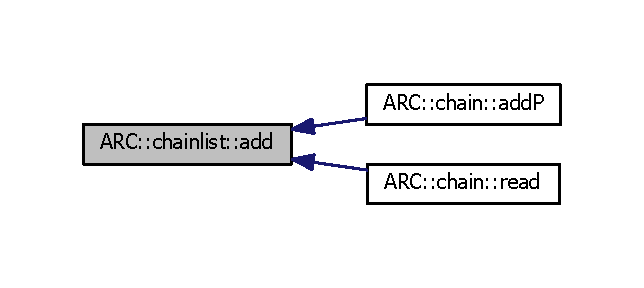
\includegraphics[width=309pt]{classARC_1_1chainlist_a598c1819d8e715ec0a24669e5bb06c6a_icgraph}
\end{center}
\end{figure}
\hypertarget{classARC_1_1chainlist_a1d73020beb10702237c27745c3ba851f}{}\label{classARC_1_1chainlist_a1d73020beb10702237c27745c3ba851f} 
\index{A\+R\+C\+::chainlist@{A\+R\+C\+::chainlist}!add@{add}}
\index{add@{add}!A\+R\+C\+::chainlist@{A\+R\+C\+::chainlist}}
\subsubsection{\texorpdfstring{add()}{add()}\hspace{0.1cm}{\footnotesize\ttfamily [2/2]}}
{\footnotesize\ttfamily template$<$class particle\+\_\+$>$ \\
template$<$class Tp $>$ \\
void \hyperlink{classARC_1_1chainlist}{A\+R\+C\+::chainlist}$<$ particle\+\_\+ $>$\+::add (\begin{DoxyParamCaption}\item[{const std\+::size\+\_\+t}]{n,  }\item[{Tp}]{a\mbox{[}$\,$\mbox{]} }\end{DoxyParamCaption})\hspace{0.3cm}{\ttfamily [inline]}}



Add a list of particles. 

A\+DD a list of particles at the end of the particle address list \#p and copy it to \#data (particle type should be derived class from particle\+\_\+) 
\begin{DoxyParams}[1]{Parameters}
\mbox{\tt in}  & {\em n} & number of new particles \\
\hline
\mbox{\tt in}  & {\em a} & array of new particles \\
\hline
\end{DoxyParams}
\hypertarget{classARC_1_1chainlist_ab212df89ec5a2e81ce7525adc04001c1}{}\label{classARC_1_1chainlist_ab212df89ec5a2e81ce7525adc04001c1} 
\index{A\+R\+C\+::chainlist@{A\+R\+C\+::chainlist}!allocate@{allocate}}
\index{allocate@{allocate}!A\+R\+C\+::chainlist@{A\+R\+C\+::chainlist}}
\subsubsection{\texorpdfstring{allocate()}{allocate()}}
{\footnotesize\ttfamily template$<$class particle\+\_\+$>$ \\
void \hyperlink{classARC_1_1chainlist}{A\+R\+C\+::chainlist}$<$ particle\+\_\+ $>$\+::allocate (\begin{DoxyParamCaption}\item[{const std\+::size\+\_\+t}]{n }\end{DoxyParamCaption})\hspace{0.3cm}{\ttfamily [inline]}}



Memory allocation of particle and particle address array. 

Set maximum particle number to {\itshape n} and allocate memory for \#p to storing the particle addresses (maximum {\itshape n}) and \#data to storing particle copies Here is the caller graph for this function\+:
\nopagebreak
\begin{figure}[H]
\begin{center}
\leavevmode
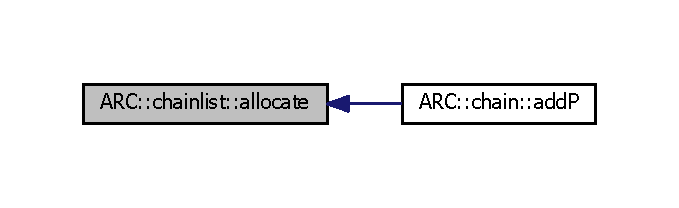
\includegraphics[width=326pt]{classARC_1_1chainlist_ab212df89ec5a2e81ce7525adc04001c1_icgraph}
\end{center}
\end{figure}
\hypertarget{classARC_1_1chainlist_af6b33790ba054657d9e132c177ed7f04}{}\label{classARC_1_1chainlist_af6b33790ba054657d9e132c177ed7f04} 
\index{A\+R\+C\+::chainlist@{A\+R\+C\+::chainlist}!clear@{clear}}
\index{clear@{clear}!A\+R\+C\+::chainlist@{A\+R\+C\+::chainlist}}
\subsubsection{\texorpdfstring{clear()}{clear()}}
{\footnotesize\ttfamily template$<$class particle\+\_\+$>$ \\
void \hyperlink{classARC_1_1chainlist}{A\+R\+C\+::chainlist}$<$ particle\+\_\+ $>$\+::clear (\begin{DoxyParamCaption}{ }\end{DoxyParamCaption})\hspace{0.3cm}{\ttfamily [inline]}}



Clear function. 

allocate memory of n particle data with type of particle class 
\begin{DoxyParams}[1]{Parameters}
\mbox{\tt in}  & {\em n} & number of particles\\
\hline
\end{DoxyParams}
Free dynamical memory space used in particle address list \#p Here is the caller graph for this function\+:
\nopagebreak
\begin{figure}[H]
\begin{center}
\leavevmode
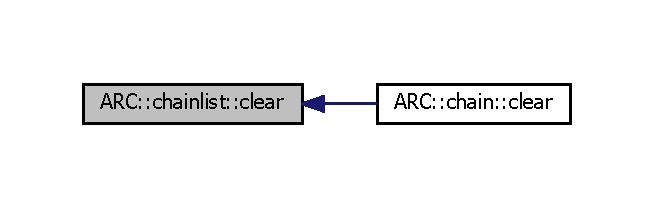
\includegraphics[width=314pt]{classARC_1_1chainlist_af6b33790ba054657d9e132c177ed7f04_icgraph}
\end{center}
\end{figure}
\hypertarget{classARC_1_1chainlist_aba70559e1b70882256a7805744e22b25}{}\label{classARC_1_1chainlist_aba70559e1b70882256a7805744e22b25} 
\index{A\+R\+C\+::chainlist@{A\+R\+C\+::chainlist}!copyback@{copyback}}
\index{copyback@{copyback}!A\+R\+C\+::chainlist@{A\+R\+C\+::chainlist}}
\subsubsection{\texorpdfstring{copyback()}{copyback()}}
{\footnotesize\ttfamily template$<$class particle\+\_\+$>$ \\
void \hyperlink{classARC_1_1chainlist}{A\+R\+C\+::chainlist}$<$ particle\+\_\+ $>$\+::copyback (\begin{DoxyParamCaption}{ }\end{DoxyParamCaption})\hspace{0.3cm}{\ttfamily [inline]}}



copy data back to original address 

! Is i$^\wedge$th a chain? $\ast$! Check whether the i$^\wedge$th member in the particle address list is chain ! Get particle list in a chain type member $\ast$! Return the address of particle list of the i$^\wedge$th member in particle \#p (A\+R\+C\+::chain.\+p)

copy the data back to original address assuming data type as particle\+\_\+ Here is the caller graph for this function\+:
\nopagebreak
\begin{figure}[H]
\begin{center}
\leavevmode
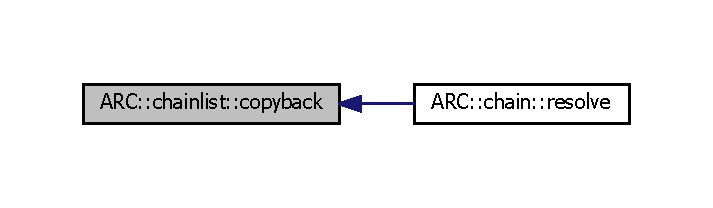
\includegraphics[width=342pt]{classARC_1_1chainlist_aba70559e1b70882256a7805744e22b25_icgraph}
\end{center}
\end{figure}
\hypertarget{classARC_1_1chainlist_a4b42fabdc7ff6edca56ce65b316f581f}{}\label{classARC_1_1chainlist_a4b42fabdc7ff6edca56ce65b316f581f} 
\index{A\+R\+C\+::chainlist@{A\+R\+C\+::chainlist}!dump@{dump}}
\index{dump@{dump}!A\+R\+C\+::chainlist@{A\+R\+C\+::chainlist}}
\subsubsection{\texorpdfstring{dump()}{dump()}}
{\footnotesize\ttfamily template$<$class particle\+\_\+$>$ \\
void \hyperlink{classARC_1_1chainlist}{A\+R\+C\+::chainlist}$<$ particle\+\_\+ $>$\+::dump (\begin{DoxyParamCaption}\item[{const char $\ast$}]{filename }\end{DoxyParamCaption})\hspace{0.3cm}{\ttfamily [inline]}}



Dump function for particle data. 

Dump particle data into file using fwrite (binary format). Number of particles is written first, then the data of particle class in the particle list \#p. 
\begin{DoxyParams}[1]{Parameters}
\mbox{\tt in}  & {\em filename} & file to store the data \\
\hline
\end{DoxyParams}
\hypertarget{classARC_1_1chainlist_a0e19bd06e5aa685e88948c947cd06552}{}\label{classARC_1_1chainlist_a0e19bd06e5aa685e88948c947cd06552} 
\index{A\+R\+C\+::chainlist@{A\+R\+C\+::chainlist}!get\+Data@{get\+Data}}
\index{get\+Data@{get\+Data}!A\+R\+C\+::chainlist@{A\+R\+C\+::chainlist}}
\subsubsection{\texorpdfstring{get\+Data()}{getData()}}
{\footnotesize\ttfamily template$<$class particle\+\_\+$>$ \\
particle$\ast$ \hyperlink{classARC_1_1chainlist}{A\+R\+C\+::chainlist}$<$ particle\+\_\+ $>$\+::get\+Data (\begin{DoxyParamCaption}{ }\end{DoxyParamCaption}) const\hspace{0.3cm}{\ttfamily [inline]}}



return particle data first pointer 

Here is the caller graph for this function\+:
\nopagebreak
\begin{figure}[H]
\begin{center}
\leavevmode
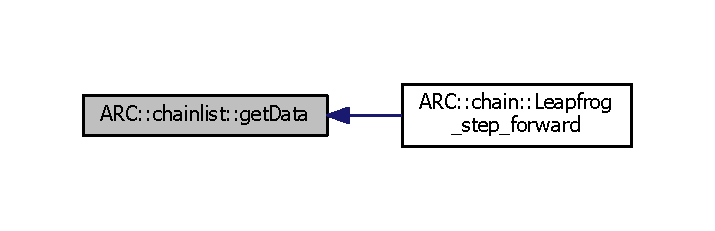
\includegraphics[width=343pt]{classARC_1_1chainlist_a0e19bd06e5aa685e88948c947cd06552_icgraph}
\end{center}
\end{figure}
\hypertarget{classARC_1_1chainlist_a85bba1921256d2a1a6784006927ad397}{}\label{classARC_1_1chainlist_a85bba1921256d2a1a6784006927ad397} 
\index{A\+R\+C\+::chainlist@{A\+R\+C\+::chainlist}!get\+Mass\+All@{get\+Mass\+All}}
\index{get\+Mass\+All@{get\+Mass\+All}!A\+R\+C\+::chainlist@{A\+R\+C\+::chainlist}}
\subsubsection{\texorpdfstring{get\+Mass\+All()}{getMassAll()}}
{\footnotesize\ttfamily template$<$class particle\+\_\+$>$ \\
void \hyperlink{classARC_1_1chainlist}{A\+R\+C\+::chainlist}$<$ particle\+\_\+ $>$\+::get\+Mass\+All (\begin{DoxyParamCaption}\item[{double}]{mass\mbox{[}$\,$\mbox{]} }\end{DoxyParamCaption})\hspace{0.3cm}{\ttfamily [inline]}}



Get particle masses and store into array. 

! Get number of chain members $\ast$! \begin{DoxyReturn}{Returns}
Number of chain members in particle address list \#p
\end{DoxyReturn}
Obtain particle masses and store into the double array 
\begin{DoxyParams}[1]{Parameters}
\mbox{\tt in}  & {\em mass} & double array to store the particle masses \\
\hline
\end{DoxyParams}
Here is the caller graph for this function\+:
\nopagebreak
\begin{figure}[H]
\begin{center}
\leavevmode
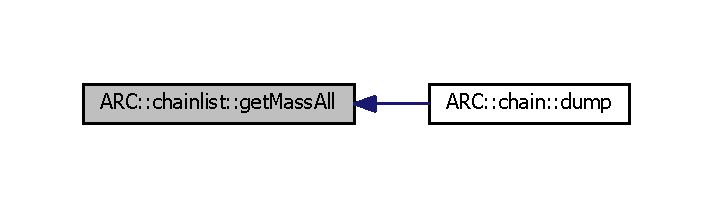
\includegraphics[width=342pt]{classARC_1_1chainlist_a85bba1921256d2a1a6784006927ad397_icgraph}
\end{center}
\end{figure}
\hypertarget{classARC_1_1chainlist_a4292d4468e5d710392f11cee0c1f01b9}{}\label{classARC_1_1chainlist_a4292d4468e5d710392f11cee0c1f01b9} 
\index{A\+R\+C\+::chainlist@{A\+R\+C\+::chainlist}!getN@{getN}}
\index{getN@{getN}!A\+R\+C\+::chainlist@{A\+R\+C\+::chainlist}}
\subsubsection{\texorpdfstring{get\+N()}{getN()}}
{\footnotesize\ttfamily template$<$class particle\+\_\+$>$ \\
std\+::size\+\_\+t \hyperlink{classARC_1_1chainlist}{A\+R\+C\+::chainlist}$<$ particle\+\_\+ $>$\+::getN (\begin{DoxyParamCaption}{ }\end{DoxyParamCaption}) const\hspace{0.3cm}{\ttfamily [inline]}}



Get current particle number. 

\begin{DoxyReturn}{Returns}
Current particle number in particle address list \#p 
\end{DoxyReturn}
Here is the caller graph for this function\+:
\nopagebreak
\begin{figure}[H]
\begin{center}
\leavevmode
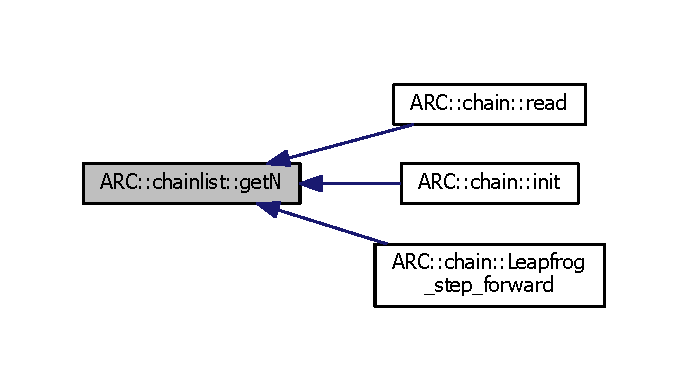
\includegraphics[width=330pt]{classARC_1_1chainlist_a4292d4468e5d710392f11cee0c1f01b9_icgraph}
\end{center}
\end{figure}
\hypertarget{classARC_1_1chainlist_a582f94629e7433bab30f7ab5e4ef588f}{}\label{classARC_1_1chainlist_a582f94629e7433bab30f7ab5e4ef588f} 
\index{A\+R\+C\+::chainlist@{A\+R\+C\+::chainlist}!get\+Nmax@{get\+Nmax}}
\index{get\+Nmax@{get\+Nmax}!A\+R\+C\+::chainlist@{A\+R\+C\+::chainlist}}
\subsubsection{\texorpdfstring{get\+Nmax()}{getNmax()}}
{\footnotesize\ttfamily template$<$class particle\+\_\+$>$ \\
std\+::size\+\_\+t \hyperlink{classARC_1_1chainlist}{A\+R\+C\+::chainlist}$<$ particle\+\_\+ $>$\+::get\+Nmax (\begin{DoxyParamCaption}{ }\end{DoxyParamCaption}) const\hspace{0.3cm}{\ttfamily [inline]}}



Get maximum particle number. 

\begin{DoxyReturn}{Returns}
Current maximum particle number that can be stored in particle address list \#p 
\end{DoxyReturn}
\hypertarget{classARC_1_1chainlist_a0e2f35b8eabe9d9ecd77ed9f24e083de}{}\label{classARC_1_1chainlist_a0e2f35b8eabe9d9ecd77ed9f24e083de} 
\index{A\+R\+C\+::chainlist@{A\+R\+C\+::chainlist}!is\+\_\+alloc@{is\+\_\+alloc}}
\index{is\+\_\+alloc@{is\+\_\+alloc}!A\+R\+C\+::chainlist@{A\+R\+C\+::chainlist}}
\subsubsection{\texorpdfstring{is\+\_\+alloc()}{is\_alloc()}}
{\footnotesize\ttfamily template$<$class particle\+\_\+$>$ \\
bool \hyperlink{classARC_1_1chainlist}{A\+R\+C\+::chainlist}$<$ particle\+\_\+ $>$\+::is\+\_\+alloc (\begin{DoxyParamCaption}{ }\end{DoxyParamCaption}) const\hspace{0.3cm}{\ttfamily [inline]}}



show whether the chainlist allocated memory 

\begin{DoxyReturn}{Returns}
if allocated, ture; otherwise false 
\end{DoxyReturn}
Here is the caller graph for this function\+:
\nopagebreak
\begin{figure}[H]
\begin{center}
\leavevmode
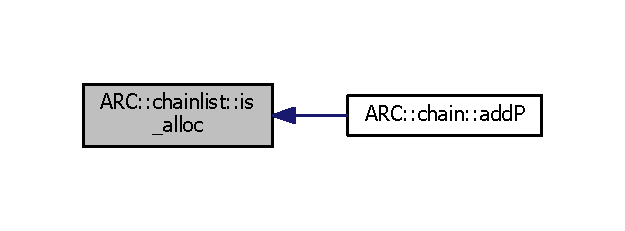
\includegraphics[width=300pt]{classARC_1_1chainlist_a0e2f35b8eabe9d9ecd77ed9f24e083de_icgraph}
\end{center}
\end{figure}
\hypertarget{classARC_1_1chainlist_aa767ec18c7ed7372a1ef1a4b27a171c3}{}\label{classARC_1_1chainlist_aa767ec18c7ed7372a1ef1a4b27a171c3} 
\index{A\+R\+C\+::chainlist@{A\+R\+C\+::chainlist}!load@{load}}
\index{load@{load}!A\+R\+C\+::chainlist@{A\+R\+C\+::chainlist}}
\subsubsection{\texorpdfstring{load()}{load()}}
{\footnotesize\ttfamily template$<$class particle\+\_\+$>$ \\
void \hyperlink{classARC_1_1chainlist}{A\+R\+C\+::chainlist}$<$ particle\+\_\+ $>$\+::load (\begin{DoxyParamCaption}\item[{const std\+::size\+\_\+t}]{n,  }\item[{particle}]{a\mbox{[}$\,$\mbox{]} }\end{DoxyParamCaption})\hspace{0.3cm}{\ttfamily [inline]}}



load a list of particles 

different from \hyperlink{classARC_1_1chainlist_a598c1819d8e715ec0a24669e5bb06c6a}{add()}, this function will directly register the first particle address and the number of particles. Thus no copies of particles are made. This is used when all particles are continued distributed in memory. This function can not be used when \hyperlink{classARC_1_1chainlist_ab212df89ec5a2e81ce7525adc04001c1}{allocate()} is already called. 
\begin{DoxyParams}[1]{Parameters}
\mbox{\tt in}  & {\em n} & number of new particles \\
\hline
\mbox{\tt in}  & {\em a} & array of new particles \\
\hline
\end{DoxyParams}
Here is the caller graph for this function\+:
\nopagebreak
\begin{figure}[H]
\begin{center}
\leavevmode
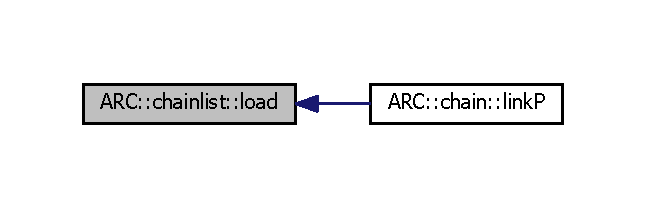
\includegraphics[width=310pt]{classARC_1_1chainlist_aa767ec18c7ed7372a1ef1a4b27a171c3_icgraph}
\end{center}
\end{figure}
\hypertarget{classARC_1_1chainlist_a995cc0dd04b7c6d8e61080db801845c1}{}\label{classARC_1_1chainlist_a995cc0dd04b7c6d8e61080db801845c1} 
\index{A\+R\+C\+::chainlist@{A\+R\+C\+::chainlist}!operator\mbox{[}\mbox{]}@{operator[]}}
\index{operator\mbox{[}\mbox{]}@{operator[]}!A\+R\+C\+::chainlist@{A\+R\+C\+::chainlist}}
\subsubsection{\texorpdfstring{operator[]()}{operator[]()}}
{\footnotesize\ttfamily template$<$class particle\+\_\+$>$ \\
particle\& \hyperlink{classARC_1_1chainlist}{A\+R\+C\+::chainlist}$<$ particle\+\_\+ $>$\+::operator\mbox{[}$\,$\mbox{]} (\begin{DoxyParamCaption}\item[{const std\+::size\+\_\+t}]{i }\end{DoxyParamCaption}) const\hspace{0.3cm}{\ttfamily [inline]}}



Return the i$^\wedge$th of memebr\textquotesingle{}s reference in the particle \#data. 

\mbox{[}\mbox{]} Operator overloading, return the i$^\wedge$th particle reference from the particle (copied) data list 
\begin{DoxyParams}[1]{Parameters}
\mbox{\tt in}  & {\em i} & the index of member in the list \#p \\
\hline
\end{DoxyParams}
\begin{DoxyReturn}{Returns}
particle reference in chainlist \#data 
\end{DoxyReturn}
\hypertarget{classARC_1_1chainlist_adfa67e2ccdbdfd7ed945fa7617f90ecc}{}\label{classARC_1_1chainlist_adfa67e2ccdbdfd7ed945fa7617f90ecc} 
\index{A\+R\+C\+::chainlist@{A\+R\+C\+::chainlist}!read@{read}}
\index{read@{read}!A\+R\+C\+::chainlist@{A\+R\+C\+::chainlist}}
\subsubsection{\texorpdfstring{read()}{read()}}
{\footnotesize\ttfamily template$<$class particle\+\_\+$>$ \\
void \hyperlink{classARC_1_1chainlist}{A\+R\+C\+::chainlist}$<$ particle\+\_\+ $>$\+::read (\begin{DoxyParamCaption}\item[{const char $\ast$}]{filename }\end{DoxyParamCaption})\hspace{0.3cm}{\ttfamily [inline]}}



Read function for particle data. 

Read particle data using fread (binary format). Number of particles should be first variable, then the data of particles (the data structure should be consistent with particle class). Notice if read is used, the particle data memory is allocated inside chainlist, this is different from \hyperlink{classARC_1_1chainlist_a598c1819d8e715ec0a24669e5bb06c6a}{add()} function. 
\begin{DoxyParams}[1]{Parameters}
\mbox{\tt in}  & {\em filename} & file to read the data \\
\hline
\end{DoxyParams}
Here is the caller graph for this function\+:
\nopagebreak
\begin{figure}[H]
\begin{center}
\leavevmode
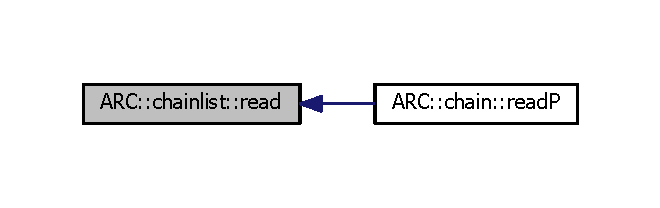
\includegraphics[width=317pt]{classARC_1_1chainlist_adfa67e2ccdbdfd7ed945fa7617f90ecc_icgraph}
\end{center}
\end{figure}
\hypertarget{classARC_1_1chainlist_adcf73b53ad0da50299f4ef3f5fefae04}{}\label{classARC_1_1chainlist_adcf73b53ad0da50299f4ef3f5fefae04} 
\index{A\+R\+C\+::chainlist@{A\+R\+C\+::chainlist}!remove@{remove}}
\index{remove@{remove}!A\+R\+C\+::chainlist@{A\+R\+C\+::chainlist}}
\subsubsection{\texorpdfstring{remove()}{remove()}}
{\footnotesize\ttfamily template$<$class particle\+\_\+$>$ \\
void \hyperlink{classARC_1_1chainlist}{A\+R\+C\+::chainlist}$<$ particle\+\_\+ $>$\+::remove (\begin{DoxyParamCaption}\item[{const std\+::size\+\_\+t}]{i,  }\item[{bool}]{option = {\ttfamily true} }\end{DoxyParamCaption})\hspace{0.3cm}{\ttfamily [inline]}}



remove one particle 

! Add a chain in particle address list \#p $\ast$! Add one chain\textquotesingle{}s address at the end of particle address list \#p

remove one particle from \#p 
\begin{DoxyParams}[1]{Parameters}
\mbox{\tt in}  & {\em i} & particle index in \#p needs to be removed \\
\hline
\mbox{\tt in}  & {\em option} & position update option\+:
\begin{DoxyItemize}
\item true\+: shift last particle to current position (defaulted);
\item false\+: shift all right particle to left by one 
\end{DoxyItemize}\\
\hline
\end{DoxyParams}
Here is the caller graph for this function\+:
\nopagebreak
\begin{figure}[H]
\begin{center}
\leavevmode
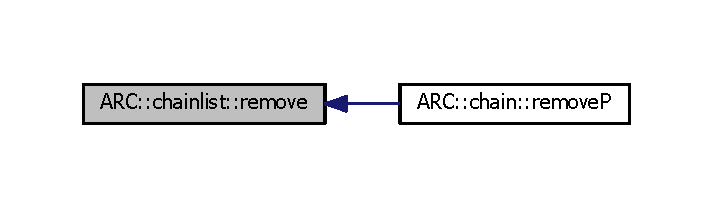
\includegraphics[width=342pt]{classARC_1_1chainlist_adcf73b53ad0da50299f4ef3f5fefae04_icgraph}
\end{center}
\end{figure}


The documentation for this class was generated from the following file\+:\begin{DoxyCompactItemize}
\item 
C\+:/\+Users/longw/\+Documents/\+Git\+Hub/\+A\+R\+C/include/\hyperlink{AR_8h}{A\+R.\+h}\end{DoxyCompactItemize}

\hypertarget{classARC_1_1chainpars}{}\section{A\+RC\+:\+:chainpars Class Reference}
\label{classARC_1_1chainpars}\index{A\+R\+C\+::chainpars@{A\+R\+C\+::chainpars}}


The chain parameter controller class.  




{\ttfamily \#include $<$A\+R.\+h$>$}

\subsection*{Public Member Functions}
\begin{DoxyCompactItemize}
\item 
\hyperlink{classARC_1_1chainpars_a2019a609d85e2b801f306ac8c7f268ab}{chainpars} ()
\begin{DoxyCompactList}\small\item\em constructor with defaulted parameters \end{DoxyCompactList}\item 
\hyperlink{classARC_1_1chainpars_a26235d742aafa97dcaad75a5db74141e}{chainpars} (const double a, const double b, const double g, const double error=1\+E-\/10, const double dtm=5.\+4e-\/20, const double dte=1e-\/6, const std\+::size\+\_\+t itermax=20, const int ext\+\_\+method=2, const int ext\+\_\+sequence=2, const int dense\+\_\+intpmax=10, const bool ext\+\_\+iteration\+\_\+const=false)
\begin{DoxyCompactList}\small\item\em constructor \end{DoxyCompactList}\item 
\hyperlink{classARC_1_1chainpars_a032873f782645efb6e60dc77f6d425dc}{$\sim$chainpars} ()
\begin{DoxyCompactList}\small\item\em destructor \end{DoxyCompactList}\item 
void \hyperlink{classARC_1_1chainpars_a37f8af288217cbfc61a3593e21976d06}{setabg} (const double a=1.\+0, const double b=0.\+0, const double g=0.\+0)
\begin{DoxyCompactList}\small\item\em Set time step transformation parameter. \end{DoxyCompactList}\item 
void \hyperlink{classARC_1_1chainpars_ad89c97941d06711adf5d46e56c5ff247}{getabg} (double \&a, double \&b, double \&g) const 
\begin{DoxyCompactList}\small\item\em Get time step transformation parameter. \end{DoxyCompactList}\item 
void \hyperlink{classARC_1_1chainpars_a59709cc9464bed3a17f99cf3fd611ad3}{set\+Err} (const double error=1\+E-\/10, const double dtm=5.\+4e-\/20, const double dte=1e-\/6)
\begin{DoxyCompactList}\small\item\em Set error paremeters. \end{DoxyCompactList}\item 
void \hyperlink{classARC_1_1chainpars_ae5946e3523a7e72d38f579e900dd20e5}{set\+Intp} (const int method=2)
\begin{DoxyCompactList}\small\item\em Set interpolation method. \end{DoxyCompactList}\item 
const int \hyperlink{classARC_1_1chainpars_a090e8199e8081235539b2ffd71cf60ef}{get\+Intp} () const 
\begin{DoxyCompactList}\small\item\em Get interpolation method index. \end{DoxyCompactList}\item 
void \hyperlink{classARC_1_1chainpars_acee4adb70778441325e76eedbdbe6343}{set\+Iter\+Const} (const bool ext\+\_\+iteration\+\_\+const=false)
\begin{DoxyCompactList}\small\item\em Set whether to use constant iteration number in extrapolation integration. \end{DoxyCompactList}\item 
void \hyperlink{classARC_1_1chainpars_a4b9a1b853f414f1dfb4ca1fc36d2178b}{set\+Iter\+Seq} (const std\+::size\+\_\+t itermax=20, const int sequence=2, const std\+::size\+\_\+t intpmax=0)
\begin{DoxyCompactList}\small\item\em Set extrapolation maximum iteration number and sequences. \end{DoxyCompactList}\item 
void \hyperlink{classARC_1_1chainpars_aa19305c22ed42da4256e968ba38df871}{set\+Den\+Intpmax} (const std\+::size\+\_\+t intpmax)
\begin{DoxyCompactList}\small\item\em set maximum derivate index for dense output interpolation \end{DoxyCompactList}\item 
const int \hyperlink{classARC_1_1chainpars_a31637df57e2c90f5435e58a08bdc1475}{get\+Den\+Intpmax} () const 
\begin{DoxyCompactList}\small\item\em Get maximum derivate index for dense output interpolation. \end{DoxyCompactList}\item 
const int \hyperlink{classARC_1_1chainpars_ae2a108596c0f621590192fbf5cd1727f}{get\+Seq} () const 
\begin{DoxyCompactList}\small\item\em Get sequence method indices. \end{DoxyCompactList}\item 
const int \hyperlink{classARC_1_1chainpars_a24ffafdeab7dfb59824a4dc3a17e5777}{get\+Iter} () const 
\begin{DoxyCompactList}\small\item\em Get extrapolation maximum iteration times (maximum sequence index) \end{DoxyCompactList}\item 
void \hyperlink{classARC_1_1chainpars_a12066ef8bca0ad69362d608959c9149b}{set\+Auto\+Step} (const int option, const double factor\+\_\+min=0.\+7, const double factor\+\_\+max=1.\+3, const double eps=0.\+125, const std\+::size\+\_\+t iter\+\_\+min=5, const std\+::size\+\_\+t iter\+\_\+max=17)
\begin{DoxyCompactList}\small\item\em Determine auto-\/step parameter. \end{DoxyCompactList}\item 
void \hyperlink{classARC_1_1chainpars_a2e5d65ea1a3b76263cad7fbd9e906e65}{get\+Auto\+Step} (int \&option, double \&factor\+\_\+min, double \&factor\+\_\+max, double \&eps, std\+::size\+\_\+t \&iter\+\_\+min, std\+::size\+\_\+t \&iter\+\_\+max) const 
\begin{DoxyCompactList}\small\item\em Get auto-\/step parameters. \end{DoxyCompactList}\item 
void \hyperlink{classARC_1_1chainpars_a96c5e40acaa2abb81e0630935eaf3ed3}{dump} (const char $\ast$filename) const 
\begin{DoxyCompactList}\small\item\em parameters dumping \end{DoxyCompactList}\item 
void \hyperlink{classARC_1_1chainpars_aa42cf56363fba1701a26cc445eda01d5}{load} (const char $\ast$filename)
\begin{DoxyCompactList}\small\item\em parameters loading from a dumped file \end{DoxyCompactList}\item 
void \hyperlink{classARC_1_1chainpars_a3bd667353d49614c52ad6c965a7480f3}{print} (std\+::ostream \&fout)
\begin{DoxyCompactList}\small\item\em Print parameter table. \end{DoxyCompactList}\end{DoxyCompactItemize}
\subsection*{Public Attributes}
\begin{DoxyCompactItemize}
\item 
double \hyperlink{classARC_1_1chainpars_ac414014d19915aecb35245ba11649c2e}{dtmin}
\begin{DoxyCompactList}\small\item\em minimum physical time step \end{DoxyCompactList}\item 
double \hyperlink{classARC_1_1chainpars_ad3a3e8f9199180ec82b9c257b1e8570e}{dterr}
\begin{DoxyCompactList}\small\item\em physical time error criterion \end{DoxyCompactList}\item 
double \hyperlink{classARC_1_1chainpars_a7ee477ebe8b1d67457891ab58560c074}{exp\+\_\+error}
\begin{DoxyCompactList}\small\item\em relative error requirement for extrapolation \end{DoxyCompactList}\item 
bool \hyperlink{classARC_1_1chainpars_a3f16e6ea9497e294265c4a17df0394ba}{exp\+\_\+fix\+\_\+iter}
\begin{DoxyCompactList}\small\item\em flag showing whether the times of iteration is fixed or not \end{DoxyCompactList}\end{DoxyCompactItemize}
\subsection*{Friends}
\begin{DoxyCompactItemize}
\item 
{\footnotesize template$<$class T $>$ }\\class \hyperlink{classARC_1_1chainpars_a498fbb4337b9878a5f0044996e4a2489}{chain}
\end{DoxyCompactItemize}


\subsection{Detailed Description}
The chain parameter controller class. 

This class control integration methods and error parameters for \hyperlink{classARC_1_1chain}{chain} 

\subsection{Constructor \& Destructor Documentation}
\index{A\+R\+C\+::chainpars@{A\+R\+C\+::chainpars}!chainpars@{chainpars}}
\index{chainpars@{chainpars}!A\+R\+C\+::chainpars@{A\+R\+C\+::chainpars}}
\subsubsection[{\texorpdfstring{chainpars()}{chainpars()}}]{\setlength{\rightskip}{0pt plus 5cm}A\+R\+C\+::chainpars\+::chainpars (
\begin{DoxyParamCaption}
{}
\end{DoxyParamCaption}
)\hspace{0.3cm}{\ttfamily [inline]}}\hypertarget{classARC_1_1chainpars_a2019a609d85e2b801f306ac8c7f268ab}{}\label{classARC_1_1chainpars_a2019a609d85e2b801f306ac8c7f268ab}


constructor with defaulted parameters 


\begin{DoxyItemize}
\item \hyperlink{namespaceARC}{A\+RC} method use logarithmic Hamiltonian (logH) (\#alpha = 1.\+0, \#beta = 0.\+0 \#gamma = 0.\+0).
\item Phase/energy error limit \hyperlink{classARC_1_1chainpars_a7ee477ebe8b1d67457891ab58560c074}{exp\+\_\+error} = 1e-\/10.
\item Minimum physical time step \hyperlink{classARC_1_1chainpars_ac414014d19915aecb35245ba11649c2e}{dtmin} = 5.\+4e-\/20.
\item Time synchronization error limit \hyperlink{classARC_1_1chainpars_ad3a3e8f9199180ec82b9c257b1e8570e}{dterr} = 1e-\/10.
\item Maximum extrapolation sequence index (accuracy order/iteration times) \#exp\+\_\+itermax = 20
\item The maximum sequence index (iteration times) is adjusted by error criterion
\item Bulirsch \& Stoer sequence \{h, h/2, h/3, h/4, h/6...\} is used
\item No auto-\/step 
\end{DoxyItemize}\index{A\+R\+C\+::chainpars@{A\+R\+C\+::chainpars}!chainpars@{chainpars}}
\index{chainpars@{chainpars}!A\+R\+C\+::chainpars@{A\+R\+C\+::chainpars}}
\subsubsection[{\texorpdfstring{chainpars(const double a, const double b, const double g, const double error=1\+E-\/10, const double dtm=5.\+4e-\/20, const double dte=1e-\/6, const std\+::size\+\_\+t itermax=20, const int ext\+\_\+method=2, const int ext\+\_\+sequence=2, const int dense\+\_\+intpmax=10, const bool ext\+\_\+iteration\+\_\+const=false)}{chainpars(const double a, const double b, const double g, const double error=1E-10, const double dtm=5.4e-20, const double dte=1e-6, const std::size_t itermax=20, const int ext_method=2, const int ext_sequence=2, const int dense_intpmax=10, const bool ext_iteration_const=false)}}]{\setlength{\rightskip}{0pt plus 5cm}A\+R\+C\+::chainpars\+::chainpars (
\begin{DoxyParamCaption}
\item[{const double}]{a, }
\item[{const double}]{b, }
\item[{const double}]{g, }
\item[{const double}]{error = {\ttfamily 1E-\/10}, }
\item[{const double}]{dtm = {\ttfamily 5.4e-\/20}, }
\item[{const double}]{dte = {\ttfamily 1e-\/6}, }
\item[{const std\+::size\+\_\+t}]{itermax = {\ttfamily 20}, }
\item[{const int}]{ext\+\_\+method = {\ttfamily 2}, }
\item[{const int}]{ext\+\_\+sequence = {\ttfamily 2}, }
\item[{const int}]{dense\+\_\+intpmax = {\ttfamily 10}, }
\item[{const bool}]{ext\+\_\+iteration\+\_\+const = {\ttfamily false}}
\end{DoxyParamCaption}
)\hspace{0.3cm}{\ttfamily [inline]}}\hypertarget{classARC_1_1chainpars_a26235d742aafa97dcaad75a5db74141e}{}\label{classARC_1_1chainpars_a26235d742aafa97dcaad75a5db74141e}


constructor 

All parameters can be set except anto-\/step method (defaulted is zero) 
\begin{DoxyParams}[1]{Parameters}
\mbox{\tt in}  & {\em a,b,g} & \hyperlink{namespaceARC}{A\+RC} time transformation method coefficients ( $ dt = ds/[a *(logH) + b * (TTL) + g])$. ~\newline

\begin{DoxyItemize}
\item a\+: Logarithmic Hamiltonian (logH) method coefficient \#alpha (0.\+0, 1.\+0)
\item b\+: Time-\/\+Transformed Leapfrog (T\+TL) method coefficient \#beta (0.\+0, 1.\+0)
\item g\+: Constant coefficient (no time transformation) \#gamma 
\end{DoxyItemize}\\
\hline
\mbox{\tt in}  & {\em error} & Phase/energy error limit (defaulted \hyperlink{classARC_1_1chainpars_a7ee477ebe8b1d67457891ab58560c074}{exp\+\_\+error} = 1e-\/10) \\
\hline
\mbox{\tt in}  & {\em dtm} & Minimum physical time step (defaulted \hyperlink{classARC_1_1chainpars_ac414014d19915aecb35245ba11649c2e}{dtmin} = 5.\+4e-\/20) \\
\hline
\mbox{\tt in}  & {\em dte} & Time synchronization error limit (defaulted \hyperlink{classARC_1_1chainpars_ad3a3e8f9199180ec82b9c257b1e8570e}{dterr} = 1e-\/6) \\
\hline
\mbox{\tt in}  & {\em itermax} & Maximum extrapolation sequence index (accuracy order/iteration times) (defaulted \#exp\+\_\+itermax = 20) \\
\hline
\mbox{\tt in}  & {\em ext\+\_\+method} & 1\+: Polynomial interpolation method; others\+: Rational interpolation method (defaulted\+: Rational) \\
\hline
\mbox{\tt in}  & {\em ext\+\_\+sequence} & 1\+: Romberg sequence \{h, h/2, h/4, h/8 ...\}; 2\+: Bulirsch \& Stoer (BS) sequence \{h, h/2, h/3, h/4, h/6, h/8 ...\}; 3\+: 4k sequence \{h, h/2, h/6, h/10, h/14 ...\}; others\+: Harmonic sequence \{h, h/2, h/3, h/4 ...\} (defaulted 2. BS sequence) \\
\hline
\mbox{\tt in}  & {\em dense\+\_\+intpmax} & maximum derivate index for dense output interpolation (defaulted \#itermax/2) \\
\hline
\mbox{\tt in}  & {\em ext\+\_\+iteration\+\_\+const} & true\+: the maximum sequence index (iteration times) is fixed to itermax; false\+: adjust the maximum sequence index by error criterion (false) \\
\hline
\end{DoxyParams}
\index{A\+R\+C\+::chainpars@{A\+R\+C\+::chainpars}!````~chainpars@{$\sim$chainpars}}
\index{````~chainpars@{$\sim$chainpars}!A\+R\+C\+::chainpars@{A\+R\+C\+::chainpars}}
\subsubsection[{\texorpdfstring{$\sim$chainpars()}{~chainpars()}}]{\setlength{\rightskip}{0pt plus 5cm}A\+R\+C\+::chainpars\+::$\sim$chainpars (
\begin{DoxyParamCaption}
{}
\end{DoxyParamCaption}
)\hspace{0.3cm}{\ttfamily [inline]}}\hypertarget{classARC_1_1chainpars_a032873f782645efb6e60dc77f6d425dc}{}\label{classARC_1_1chainpars_a032873f782645efb6e60dc77f6d425dc}


destructor 



\subsection{Member Function Documentation}
\index{A\+R\+C\+::chainpars@{A\+R\+C\+::chainpars}!dump@{dump}}
\index{dump@{dump}!A\+R\+C\+::chainpars@{A\+R\+C\+::chainpars}}
\subsubsection[{\texorpdfstring{dump(const char $\ast$filename) const }{dump(const char *filename) const }}]{\setlength{\rightskip}{0pt plus 5cm}void A\+R\+C\+::chainpars\+::dump (
\begin{DoxyParamCaption}
\item[{const char $\ast$}]{filename}
\end{DoxyParamCaption}
) const\hspace{0.3cm}{\ttfamily [inline]}}\hypertarget{classARC_1_1chainpars_a96c5e40acaa2abb81e0630935eaf3ed3}{}\label{classARC_1_1chainpars_a96c5e40acaa2abb81e0630935eaf3ed3}


parameters dumping 

Dump parameters into file. Notice dynamic array data will not be dumped. The dumping data includes\+: \#alpha, \#beta, \#gamma, \#exp\+\_\+method, \#exp\+\_\+sequence, \#exp\+\_\+itermax, \hyperlink{classARC_1_1chainpars_a7ee477ebe8b1d67457891ab58560c074}{exp\+\_\+error}, \hyperlink{classARC_1_1chainpars_a3f16e6ea9497e294265c4a17df0394ba}{exp\+\_\+fix\+\_\+iter}, \hyperlink{classARC_1_1chainpars_ac414014d19915aecb35245ba11649c2e}{dtmin}, \hyperlink{classARC_1_1chainpars_ad3a3e8f9199180ec82b9c257b1e8570e}{dterr}, \#auto\+\_\+step, auto\+\_\+step parameters 
\begin{DoxyParams}[1]{Parameters}
\mbox{\tt in}  & {\em filename} & file for storing the data \\
\hline
\end{DoxyParams}
\index{A\+R\+C\+::chainpars@{A\+R\+C\+::chainpars}!getabg@{getabg}}
\index{getabg@{getabg}!A\+R\+C\+::chainpars@{A\+R\+C\+::chainpars}}
\subsubsection[{\texorpdfstring{getabg(double \&a, double \&b, double \&g) const }{getabg(double &a, double &b, double &g) const }}]{\setlength{\rightskip}{0pt plus 5cm}void A\+R\+C\+::chainpars\+::getabg (
\begin{DoxyParamCaption}
\item[{double \&}]{a, }
\item[{double \&}]{b, }
\item[{double \&}]{g}
\end{DoxyParamCaption}
) const\hspace{0.3cm}{\ttfamily [inline]}}\hypertarget{classARC_1_1chainpars_ad89c97941d06711adf5d46e56c5ff247}{}\label{classARC_1_1chainpars_ad89c97941d06711adf5d46e56c5ff247}


Get time step transformation parameter. 

Get parameter a,b,g where physical time step $ dt = ds/[a *(logH) + b * (TTL) + g]$ ~\newline

\begin{DoxyParams}[1]{Parameters}
\mbox{\tt in}  & {\em a} & Logarithmic Hamiltonian (logH) method coefficient \#alpha (0.\+0, 1.\+0) \\
\hline
\mbox{\tt in}  & {\em b} & Time-\/\+Transformed Leapfrog (T\+TL) method coefficient \#beta (0.\+0, 1.\+0) \\
\hline
\mbox{\tt in}  & {\em g} & Constant coefficient (no time transformation) \#gamma \\
\hline
\end{DoxyParams}
\index{A\+R\+C\+::chainpars@{A\+R\+C\+::chainpars}!get\+Auto\+Step@{get\+Auto\+Step}}
\index{get\+Auto\+Step@{get\+Auto\+Step}!A\+R\+C\+::chainpars@{A\+R\+C\+::chainpars}}
\subsubsection[{\texorpdfstring{get\+Auto\+Step(int \&option, double \&factor\+\_\+min, double \&factor\+\_\+max, double \&eps, std\+::size\+\_\+t \&iter\+\_\+min, std\+::size\+\_\+t \&iter\+\_\+max) const }{getAutoStep(int &option, double &factor_min, double &factor_max, double &eps, std::size_t &iter_min, std::size_t &iter_max) const }}]{\setlength{\rightskip}{0pt plus 5cm}void A\+R\+C\+::chainpars\+::get\+Auto\+Step (
\begin{DoxyParamCaption}
\item[{int \&}]{option, }
\item[{double \&}]{factor\+\_\+min, }
\item[{double \&}]{factor\+\_\+max, }
\item[{double \&}]{eps, }
\item[{std\+::size\+\_\+t \&}]{iter\+\_\+min, }
\item[{std\+::size\+\_\+t \&}]{iter\+\_\+max}
\end{DoxyParamCaption}
) const\hspace{0.3cm}{\ttfamily [inline]}}\hypertarget{classARC_1_1chainpars_a2e5d65ea1a3b76263cad7fbd9e906e65}{}\label{classARC_1_1chainpars_a2e5d65ea1a3b76263cad7fbd9e906e65}


Get auto-\/step parameters. 


\begin{DoxyParams}[1]{Parameters}
\mbox{\tt in}  & {\em option} & auto-\/step method
\begin{DoxyItemize}
\item 0. no auto-\/step
\item 1. use extrapolation error to estimate next step
\item 2. use min( $X/(gV)$, $V/(gA)$) to estimate next step
\item 3\+: use maximum sequence index to control next step. If index $>${\itshape iter\+\_\+max}, modification factor = {\itshape factor\+\_\+min}; if index $<$ {\itshape iter\+\_\+min}, modification factor = {\itshape factor\+\_\+max};
\item 4\+: use mimimum user-\/defined two-\/body timescale of every two neigbor members to estimate next step 
\end{DoxyItemize}\\
\hline
\mbox{\tt in}  & {\em factor\+\_\+min} & if {\itshape option} = 1-\/$>$3, it is the minimum step reduction factor (defaulted\+: 0.\+7) \\
\hline
\mbox{\tt in}  & {\em factor\+\_\+max} & if {\itshape option} = 1-\/$>$3, it is the maximum step reduction factor (defaulted\+: 1.\+3) \\
\hline
\mbox{\tt in}  & {\em eps} & coefficient. If {\itshape option} = 2 or 4, coefficient is the multiplying factor for the estimated next step (defaulted\+: 0.\+125) \\
\hline
\mbox{\tt in}  & {\em iter\+\_\+min} & if {\itshape option} = 3, it is the minimum sequence index (iteration times) criterion during extrapolation intergration (defaulted\+: 5) \\
\hline
\mbox{\tt in}  & {\em iter\+\_\+max} & if {\itshape option} = 3, it is the maximum sequence index (iteration times) criterion during extrapolation intergration (defaulted\+: 17) \\
\hline
\end{DoxyParams}
\index{A\+R\+C\+::chainpars@{A\+R\+C\+::chainpars}!get\+Den\+Intpmax@{get\+Den\+Intpmax}}
\index{get\+Den\+Intpmax@{get\+Den\+Intpmax}!A\+R\+C\+::chainpars@{A\+R\+C\+::chainpars}}
\subsubsection[{\texorpdfstring{get\+Den\+Intpmax() const }{getDenIntpmax() const }}]{\setlength{\rightskip}{0pt plus 5cm}const int A\+R\+C\+::chainpars\+::get\+Den\+Intpmax (
\begin{DoxyParamCaption}
{}
\end{DoxyParamCaption}
) const\hspace{0.3cm}{\ttfamily [inline]}}\hypertarget{classARC_1_1chainpars_a31637df57e2c90f5435e58a08bdc1475}{}\label{classARC_1_1chainpars_a31637df57e2c90f5435e58a08bdc1475}


Get maximum derivate index for dense output interpolation. 

\begin{DoxyReturn}{Returns}
maximum derivate index for dense ouput interpolation (defaulted \#itermax/2) 
\end{DoxyReturn}
\index{A\+R\+C\+::chainpars@{A\+R\+C\+::chainpars}!get\+Intp@{get\+Intp}}
\index{get\+Intp@{get\+Intp}!A\+R\+C\+::chainpars@{A\+R\+C\+::chainpars}}
\subsubsection[{\texorpdfstring{get\+Intp() const }{getIntp() const }}]{\setlength{\rightskip}{0pt plus 5cm}const int A\+R\+C\+::chainpars\+::get\+Intp (
\begin{DoxyParamCaption}
{}
\end{DoxyParamCaption}
) const\hspace{0.3cm}{\ttfamily [inline]}}\hypertarget{classARC_1_1chainpars_a090e8199e8081235539b2ffd71cf60ef}{}\label{classARC_1_1chainpars_a090e8199e8081235539b2ffd71cf60ef}


Get interpolation method index. 

\begin{DoxyReturn}{Returns}
method index\+: 1\+: Polynomial method; others\+: Rational interpolation method (defaulted Rational) 
\end{DoxyReturn}
\index{A\+R\+C\+::chainpars@{A\+R\+C\+::chainpars}!get\+Iter@{get\+Iter}}
\index{get\+Iter@{get\+Iter}!A\+R\+C\+::chainpars@{A\+R\+C\+::chainpars}}
\subsubsection[{\texorpdfstring{get\+Iter() const }{getIter() const }}]{\setlength{\rightskip}{0pt plus 5cm}const int A\+R\+C\+::chainpars\+::get\+Iter (
\begin{DoxyParamCaption}
{}
\end{DoxyParamCaption}
) const\hspace{0.3cm}{\ttfamily [inline]}}\hypertarget{classARC_1_1chainpars_a24ffafdeab7dfb59824a4dc3a17e5777}{}\label{classARC_1_1chainpars_a24ffafdeab7dfb59824a4dc3a17e5777}


Get extrapolation maximum iteration times (maximum sequence index) 

\index{A\+R\+C\+::chainpars@{A\+R\+C\+::chainpars}!get\+Seq@{get\+Seq}}
\index{get\+Seq@{get\+Seq}!A\+R\+C\+::chainpars@{A\+R\+C\+::chainpars}}
\subsubsection[{\texorpdfstring{get\+Seq() const }{getSeq() const }}]{\setlength{\rightskip}{0pt plus 5cm}const int A\+R\+C\+::chainpars\+::get\+Seq (
\begin{DoxyParamCaption}
{}
\end{DoxyParamCaption}
) const\hspace{0.3cm}{\ttfamily [inline]}}\hypertarget{classARC_1_1chainpars_ae2a108596c0f621590192fbf5cd1727f}{}\label{classARC_1_1chainpars_ae2a108596c0f621590192fbf5cd1727f}


Get sequence method indices. 

\index{A\+R\+C\+::chainpars@{A\+R\+C\+::chainpars}!load@{load}}
\index{load@{load}!A\+R\+C\+::chainpars@{A\+R\+C\+::chainpars}}
\subsubsection[{\texorpdfstring{load(const char $\ast$filename)}{load(const char *filename)}}]{\setlength{\rightskip}{0pt plus 5cm}void A\+R\+C\+::chainpars\+::load (
\begin{DoxyParamCaption}
\item[{const char $\ast$}]{filename}
\end{DoxyParamCaption}
)\hspace{0.3cm}{\ttfamily [inline]}}\hypertarget{classARC_1_1chainpars_aa42cf56363fba1701a26cc445eda01d5}{}\label{classARC_1_1chainpars_aa42cf56363fba1701a26cc445eda01d5}


parameters loading from a dumped file 

Load parameters from a dumped file. All dynamical array will be initialized after reading parameters. Notice this function will load all parameters except acceleration function pointers \#pp\+\_\+\+AW and \#pp\+\_\+\+Ap. set\+A() should be called before chain integration. The reading data list is shown in \hyperlink{classARC_1_1chainpars_a96c5e40acaa2abb81e0630935eaf3ed3}{dump()} 
\begin{DoxyParams}[1]{Parameters}
\mbox{\tt in}  & {\em filename} & file to read the data \\
\hline
\end{DoxyParams}
\index{A\+R\+C\+::chainpars@{A\+R\+C\+::chainpars}!print@{print}}
\index{print@{print}!A\+R\+C\+::chainpars@{A\+R\+C\+::chainpars}}
\subsubsection[{\texorpdfstring{print(std\+::ostream \&fout)}{print(std::ostream &fout)}}]{\setlength{\rightskip}{0pt plus 5cm}void A\+R\+C\+::chainpars\+::print (
\begin{DoxyParamCaption}
\item[{std\+::ostream \&}]{fout}
\end{DoxyParamCaption}
)\hspace{0.3cm}{\ttfamily [inline]}}\hypertarget{classARC_1_1chainpars_a3bd667353d49614c52ad6c965a7480f3}{}\label{classARC_1_1chainpars_a3bd667353d49614c52ad6c965a7480f3}


Print parameter table. 

Print parameter table 
\begin{DoxyParams}[1]{Parameters}
\mbox{\tt in}  & {\em fout} & ofstream for printing \\
\hline
\end{DoxyParams}
\index{A\+R\+C\+::chainpars@{A\+R\+C\+::chainpars}!setabg@{setabg}}
\index{setabg@{setabg}!A\+R\+C\+::chainpars@{A\+R\+C\+::chainpars}}
\subsubsection[{\texorpdfstring{setabg(const double a=1.\+0, const double b=0.\+0, const double g=0.\+0)}{setabg(const double a=1.0, const double b=0.0, const double g=0.0)}}]{\setlength{\rightskip}{0pt plus 5cm}void A\+R\+C\+::chainpars\+::setabg (
\begin{DoxyParamCaption}
\item[{const double}]{a = {\ttfamily 1.0}, }
\item[{const double}]{b = {\ttfamily 0.0}, }
\item[{const double}]{g = {\ttfamily 0.0}}
\end{DoxyParamCaption}
)\hspace{0.3cm}{\ttfamily [inline]}}\hypertarget{classARC_1_1chainpars_a37f8af288217cbfc61a3593e21976d06}{}\label{classARC_1_1chainpars_a37f8af288217cbfc61a3593e21976d06}


Set time step transformation parameter. 

! Set acceleration, potential, time transformation function $\partial W/\partial r$ and $W$ calculator $\ast$! Set acceleration, potential, time transformation function $\partial W/\partial r$ and $W$ for two particles. This is the basic functions used for interaction between chain members and from perturbers.

Set parameter a,b,g where physical time step $ dt = ds/[a *(logH) + b * (TTL) + g]$ ~\newline

\begin{DoxyParams}[1]{Parameters}
\mbox{\tt in}  & {\em a} & Logarithmic Hamiltonian (logH) method coefficient \#alpha (0.\+0, 1.\+0) \\
\hline
\mbox{\tt in}  & {\em b} & Time-\/\+Transformed Leapfrog (T\+TL) method coefficient \#beta (0.\+0, 1.\+0) \\
\hline
\mbox{\tt in}  & {\em g} & Constant coefficient (no time transformation) \#gamma \\
\hline
\end{DoxyParams}
\index{A\+R\+C\+::chainpars@{A\+R\+C\+::chainpars}!set\+Auto\+Step@{set\+Auto\+Step}}
\index{set\+Auto\+Step@{set\+Auto\+Step}!A\+R\+C\+::chainpars@{A\+R\+C\+::chainpars}}
\subsubsection[{\texorpdfstring{set\+Auto\+Step(const int option, const double factor\+\_\+min=0.\+7, const double factor\+\_\+max=1.\+3, const double eps=0.\+125, const std\+::size\+\_\+t iter\+\_\+min=5, const std\+::size\+\_\+t iter\+\_\+max=17)}{setAutoStep(const int option, const double factor_min=0.7, const double factor_max=1.3, const double eps=0.125, const std::size_t iter_min=5, const std::size_t iter_max=17)}}]{\setlength{\rightskip}{0pt plus 5cm}void A\+R\+C\+::chainpars\+::set\+Auto\+Step (
\begin{DoxyParamCaption}
\item[{const int}]{option, }
\item[{const double}]{factor\+\_\+min = {\ttfamily 0.7}, }
\item[{const double}]{factor\+\_\+max = {\ttfamily 1.3}, }
\item[{const double}]{eps = {\ttfamily 0.125}, }
\item[{const std\+::size\+\_\+t}]{iter\+\_\+min = {\ttfamily 5}, }
\item[{const std\+::size\+\_\+t}]{iter\+\_\+max = {\ttfamily 17}}
\end{DoxyParamCaption}
)\hspace{0.3cm}{\ttfamily [inline]}}\hypertarget{classARC_1_1chainpars_a12066ef8bca0ad69362d608959c9149b}{}\label{classARC_1_1chainpars_a12066ef8bca0ad69362d608959c9149b}


Determine auto-\/step parameter. 


\begin{DoxyParams}[1]{Parameters}
\mbox{\tt in}  & {\em option} & auto-\/step method
\begin{DoxyItemize}
\item 0. no auto-\/step
\item 1. use extrapolation error to estimate next step
\item 2. use min( $X/(gV)$, $V/(gA)$) to estimate next step
\item 3\+: use maximum sequence index to control next step. If index $>${\itshape iter\+\_\+max}, modification factor = {\itshape factor\+\_\+min}; if index $<$ {\itshape iter\+\_\+min}, modification factor = {\itshape factor\+\_\+max};
\item 4\+: use mimimum user-\/defined two-\/body timescale of every two neigbor members to estimate next step 
\end{DoxyItemize}\\
\hline
\mbox{\tt in}  & {\em factor\+\_\+min} & if {\itshape option} = 1-\/$>$3, it is the minimum step reduction factor (defaulted\+: 0.\+7) \\
\hline
\mbox{\tt in}  & {\em factor\+\_\+max} & if {\itshape option} = 1-\/$>$3, it is the maximum step reduction factor (defaulted\+: 1.\+3) \\
\hline
\mbox{\tt in}  & {\em eps} & coefficient. If {\itshape option} = 2 or 4, coefficient is the multiplying factor for the estimated next step (defaulted\+: 0.\+125) \\
\hline
\mbox{\tt in}  & {\em iter\+\_\+min} & if {\itshape option} = 3, it is the minimum sequence index (iteration times) criterion during extrapolation intergration (defaulted\+: 5) \\
\hline
\mbox{\tt in}  & {\em iter\+\_\+max} & if {\itshape option} = 3, it is the maximum sequence index (iteration times) criterion during extrapolation intergration (defaulted\+: 17) \\
\hline
\end{DoxyParams}
\index{A\+R\+C\+::chainpars@{A\+R\+C\+::chainpars}!set\+Den\+Intpmax@{set\+Den\+Intpmax}}
\index{set\+Den\+Intpmax@{set\+Den\+Intpmax}!A\+R\+C\+::chainpars@{A\+R\+C\+::chainpars}}
\subsubsection[{\texorpdfstring{set\+Den\+Intpmax(const std\+::size\+\_\+t intpmax)}{setDenIntpmax(const std::size_t intpmax)}}]{\setlength{\rightskip}{0pt plus 5cm}void A\+R\+C\+::chainpars\+::set\+Den\+Intpmax (
\begin{DoxyParamCaption}
\item[{const std\+::size\+\_\+t}]{intpmax}
\end{DoxyParamCaption}
)\hspace{0.3cm}{\ttfamily [inline]}}\hypertarget{classARC_1_1chainpars_aa19305c22ed42da4256e968ba38df871}{}\label{classARC_1_1chainpars_aa19305c22ed42da4256e968ba38df871}


set maximum derivate index for dense output interpolation 


\begin{DoxyParams}[1]{Parameters}
\mbox{\tt in}  & {\em intpmax} & maximum derivate index for dense ouput interpolation (defaulted \#itermax/2) \\
\hline
\end{DoxyParams}
\index{A\+R\+C\+::chainpars@{A\+R\+C\+::chainpars}!set\+Err@{set\+Err}}
\index{set\+Err@{set\+Err}!A\+R\+C\+::chainpars@{A\+R\+C\+::chainpars}}
\subsubsection[{\texorpdfstring{set\+Err(const double error=1\+E-\/10, const double dtm=5.\+4e-\/20, const double dte=1e-\/6)}{setErr(const double error=1E-10, const double dtm=5.4e-20, const double dte=1e-6)}}]{\setlength{\rightskip}{0pt plus 5cm}void A\+R\+C\+::chainpars\+::set\+Err (
\begin{DoxyParamCaption}
\item[{const double}]{error = {\ttfamily 1E-\/10}, }
\item[{const double}]{dtm = {\ttfamily 5.4e-\/20}, }
\item[{const double}]{dte = {\ttfamily 1e-\/6}}
\end{DoxyParamCaption}
)\hspace{0.3cm}{\ttfamily [inline]}}\hypertarget{classARC_1_1chainpars_a59709cc9464bed3a17f99cf3fd611ad3}{}\label{classARC_1_1chainpars_a59709cc9464bed3a17f99cf3fd611ad3}


Set error paremeters. 


\begin{DoxyParams}[1]{Parameters}
\mbox{\tt in}  & {\em error} & phase/energy relative error requirement for extrapolation (defaulted \hyperlink{classARC_1_1chainpars_a7ee477ebe8b1d67457891ab58560c074}{exp\+\_\+error} = 1e-\/10) \\
\hline
\mbox{\tt in}  & {\em dtm} & minimum physical time step allown (defaulted \hyperlink{classARC_1_1chainpars_ac414014d19915aecb35245ba11649c2e}{dtmin} = 5.\+4e-\/20) \\
\hline
\mbox{\tt in}  & {\em dte} & Time synchronization error limit (defaulted \hyperlink{classARC_1_1chainpars_ad3a3e8f9199180ec82b9c257b1e8570e}{dterr} = 1e-\/6) \\
\hline
\end{DoxyParams}
\index{A\+R\+C\+::chainpars@{A\+R\+C\+::chainpars}!set\+Intp@{set\+Intp}}
\index{set\+Intp@{set\+Intp}!A\+R\+C\+::chainpars@{A\+R\+C\+::chainpars}}
\subsubsection[{\texorpdfstring{set\+Intp(const int method=2)}{setIntp(const int method=2)}}]{\setlength{\rightskip}{0pt plus 5cm}void A\+R\+C\+::chainpars\+::set\+Intp (
\begin{DoxyParamCaption}
\item[{const int}]{method = {\ttfamily 2}}
\end{DoxyParamCaption}
)\hspace{0.3cm}{\ttfamily [inline]}}\hypertarget{classARC_1_1chainpars_ae5946e3523a7e72d38f579e900dd20e5}{}\label{classARC_1_1chainpars_ae5946e3523a7e72d38f579e900dd20e5}


Set interpolation method. 

Set interpolation method for extrapolation integration 
\begin{DoxyParams}[1]{Parameters}
\mbox{\tt in}  & {\em method} & 1\+: Polynomial method; others\+: Rational interpolation method (defaulted Rational) \\
\hline
\end{DoxyParams}
\index{A\+R\+C\+::chainpars@{A\+R\+C\+::chainpars}!set\+Iter\+Const@{set\+Iter\+Const}}
\index{set\+Iter\+Const@{set\+Iter\+Const}!A\+R\+C\+::chainpars@{A\+R\+C\+::chainpars}}
\subsubsection[{\texorpdfstring{set\+Iter\+Const(const bool ext\+\_\+iteration\+\_\+const=false)}{setIterConst(const bool ext_iteration_const=false)}}]{\setlength{\rightskip}{0pt plus 5cm}void A\+R\+C\+::chainpars\+::set\+Iter\+Const (
\begin{DoxyParamCaption}
\item[{const bool}]{ext\+\_\+iteration\+\_\+const = {\ttfamily false}}
\end{DoxyParamCaption}
)\hspace{0.3cm}{\ttfamily [inline]}}\hypertarget{classARC_1_1chainpars_acee4adb70778441325e76eedbdbe6343}{}\label{classARC_1_1chainpars_acee4adb70778441325e76eedbdbe6343}


Set whether to use constant iteration number in extrapolation integration. 


\begin{DoxyParams}[1]{Parameters}
\mbox{\tt in}  & {\em ext\+\_\+iteration\+\_\+const} & true\+: the maximum sequence index (iteration times) is fixed to itermax; false\+: adjust the maximum sequence index by error criterion (false) \\
\hline
\end{DoxyParams}
\index{A\+R\+C\+::chainpars@{A\+R\+C\+::chainpars}!set\+Iter\+Seq@{set\+Iter\+Seq}}
\index{set\+Iter\+Seq@{set\+Iter\+Seq}!A\+R\+C\+::chainpars@{A\+R\+C\+::chainpars}}
\subsubsection[{\texorpdfstring{set\+Iter\+Seq(const std\+::size\+\_\+t itermax=20, const int sequence=2, const std\+::size\+\_\+t intpmax=0)}{setIterSeq(const std::size_t itermax=20, const int sequence=2, const std::size_t intpmax=0)}}]{\setlength{\rightskip}{0pt plus 5cm}void A\+R\+C\+::chainpars\+::set\+Iter\+Seq (
\begin{DoxyParamCaption}
\item[{const std\+::size\+\_\+t}]{itermax = {\ttfamily 20}, }
\item[{const int}]{sequence = {\ttfamily 2}, }
\item[{const std\+::size\+\_\+t}]{intpmax = {\ttfamily 0}}
\end{DoxyParamCaption}
)\hspace{0.3cm}{\ttfamily [inline]}}\hypertarget{classARC_1_1chainpars_a4b9a1b853f414f1dfb4ca1fc36d2178b}{}\label{classARC_1_1chainpars_a4b9a1b853f414f1dfb4ca1fc36d2178b}


Set extrapolation maximum iteration number and sequences. 


\begin{DoxyParams}[1]{Parameters}
\mbox{\tt in}  & {\em itermax} & Maximum extrapolation sequence index (accuracy order/iteration times) (defaulted \#exp\+\_\+itermax = 20) \\
\hline
\mbox{\tt in}  & {\em sequence} & 1\+: Romberg sequence \{h, h/2, h/4, h/8 ...\}; 2\+: Bulirsch \& Stoer (BS) sequence \{h, h/2, h/3, h/4, h/6, h/8 ...\}; 3\+: 4k sequence \{h, h/2, h/6, h/10, h/14 ...\}; others\+: Harmonic sequence \{h, h/2, h/3, h/4 ...\} (defaulted 2. BS sequence) \\
\hline
\mbox{\tt in}  & {\em intpmax} & maximum derivate index for dense ouput interpolation (defaulted \#itermax/2) \\
\hline
\end{DoxyParams}


Here is the call graph for this function\+:\nopagebreak
\begin{figure}[H]
\begin{center}
\leavevmode
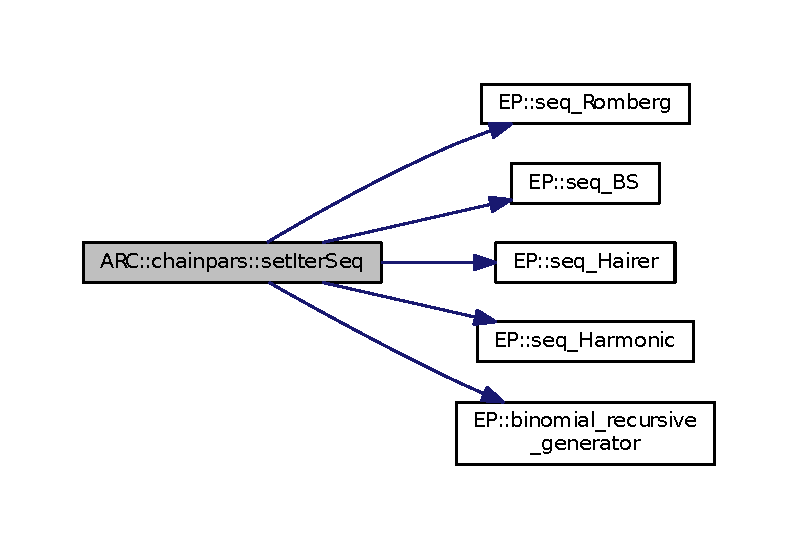
\includegraphics[width=350pt]{classARC_1_1chainpars_a4b9a1b853f414f1dfb4ca1fc36d2178b_cgraph}
\end{center}
\end{figure}




\subsection{Friends And Related Function Documentation}
\index{A\+R\+C\+::chainpars@{A\+R\+C\+::chainpars}!chain@{chain}}
\index{chain@{chain}!A\+R\+C\+::chainpars@{A\+R\+C\+::chainpars}}
\subsubsection[{\texorpdfstring{chain}{chain}}]{\setlength{\rightskip}{0pt plus 5cm}template$<$class T $>$ friend class {\bf chain}\hspace{0.3cm}{\ttfamily [friend]}}\hypertarget{classARC_1_1chainpars_a498fbb4337b9878a5f0044996e4a2489}{}\label{classARC_1_1chainpars_a498fbb4337b9878a5f0044996e4a2489}


\subsection{Member Data Documentation}
\index{A\+R\+C\+::chainpars@{A\+R\+C\+::chainpars}!dterr@{dterr}}
\index{dterr@{dterr}!A\+R\+C\+::chainpars@{A\+R\+C\+::chainpars}}
\subsubsection[{\texorpdfstring{dterr}{dterr}}]{\setlength{\rightskip}{0pt plus 5cm}double A\+R\+C\+::chainpars\+::dterr}\hypertarget{classARC_1_1chainpars_ad3a3e8f9199180ec82b9c257b1e8570e}{}\label{classARC_1_1chainpars_ad3a3e8f9199180ec82b9c257b1e8570e}


physical time error criterion 

\index{A\+R\+C\+::chainpars@{A\+R\+C\+::chainpars}!dtmin@{dtmin}}
\index{dtmin@{dtmin}!A\+R\+C\+::chainpars@{A\+R\+C\+::chainpars}}
\subsubsection[{\texorpdfstring{dtmin}{dtmin}}]{\setlength{\rightskip}{0pt plus 5cm}double A\+R\+C\+::chainpars\+::dtmin}\hypertarget{classARC_1_1chainpars_ac414014d19915aecb35245ba11649c2e}{}\label{classARC_1_1chainpars_ac414014d19915aecb35245ba11649c2e}


minimum physical time step 

\index{A\+R\+C\+::chainpars@{A\+R\+C\+::chainpars}!exp\+\_\+error@{exp\+\_\+error}}
\index{exp\+\_\+error@{exp\+\_\+error}!A\+R\+C\+::chainpars@{A\+R\+C\+::chainpars}}
\subsubsection[{\texorpdfstring{exp\+\_\+error}{exp_error}}]{\setlength{\rightskip}{0pt plus 5cm}double A\+R\+C\+::chainpars\+::exp\+\_\+error}\hypertarget{classARC_1_1chainpars_a7ee477ebe8b1d67457891ab58560c074}{}\label{classARC_1_1chainpars_a7ee477ebe8b1d67457891ab58560c074}


relative error requirement for extrapolation 

\index{A\+R\+C\+::chainpars@{A\+R\+C\+::chainpars}!exp\+\_\+fix\+\_\+iter@{exp\+\_\+fix\+\_\+iter}}
\index{exp\+\_\+fix\+\_\+iter@{exp\+\_\+fix\+\_\+iter}!A\+R\+C\+::chainpars@{A\+R\+C\+::chainpars}}
\subsubsection[{\texorpdfstring{exp\+\_\+fix\+\_\+iter}{exp_fix_iter}}]{\setlength{\rightskip}{0pt plus 5cm}bool A\+R\+C\+::chainpars\+::exp\+\_\+fix\+\_\+iter}\hypertarget{classARC_1_1chainpars_a3f16e6ea9497e294265c4a17df0394ba}{}\label{classARC_1_1chainpars_a3f16e6ea9497e294265c4a17df0394ba}


flag showing whether the times of iteration is fixed or not 



The documentation for this class was generated from the following file\+:\begin{DoxyCompactItemize}
\item 
/mnt/c/\+Users/longw/\+Documents/\+Git\+Hub/\+A\+R\+C/include/\hyperlink{AR_8h}{A\+R.\+h}\end{DoxyCompactItemize}

\hypertarget{classNTA_1_1Newtonian__pars}{}\section{N\+TA\+:\+:Newtonian\+\_\+pars Class Reference}
\label{classNTA_1_1Newtonian__pars}\index{N\+T\+A\+::\+Newtonian\+\_\+pars@{N\+T\+A\+::\+Newtonian\+\_\+pars}}


Newtonian Interaction and time transformation function parameter class.  




{\ttfamily \#include $<$Newtonian\+\_\+acceleration.\+h$>$}

\subsection*{Public Member Functions}
\begin{DoxyCompactItemize}
\item 
\hyperlink{classNTA_1_1Newtonian__pars_a350f6c6c5eaec1520604955ee32cd94b}{Newtonian\+\_\+pars} ()
\begin{DoxyCompactList}\small\item\em adjustment parameter \end{DoxyCompactList}\item 
void \hyperlink{classNTA_1_1Newtonian__pars_ae447dcfbd1da0436db3684be1e19734d}{calc\+\_\+mm2} (const double mass\mbox{[}$\,$\mbox{]}, const std\+::size\+\_\+t n)
\begin{DoxyCompactList}\small\item\em Calculate smooth particle coefficient. \end{DoxyCompactList}\end{DoxyCompactItemize}
\subsection*{Public Attributes}
\begin{DoxyCompactItemize}
\item 
double \hyperlink{classNTA_1_1Newtonian__pars_a2dbcde3115bdf43e8fcec4626e7ee5bb}{mm2}
\item 
double \hyperlink{classNTA_1_1Newtonian__pars_a4c4f79cd0d1600f8f038cdec15981268}{epi}
\begin{DoxyCompactList}\small\item\em smooth particle coefficient \end{DoxyCompactList}\end{DoxyCompactItemize}


\subsection{Detailed Description}
Newtonian Interaction and time transformation function parameter class. 

This class store the smooth mass coefficients for T\+TL methods 

\subsection{Constructor \& Destructor Documentation}
\hypertarget{classNTA_1_1Newtonian__pars_a350f6c6c5eaec1520604955ee32cd94b}{}\label{classNTA_1_1Newtonian__pars_a350f6c6c5eaec1520604955ee32cd94b} 
\index{N\+T\+A\+::\+Newtonian\+\_\+pars@{N\+T\+A\+::\+Newtonian\+\_\+pars}!Newtonian\+\_\+pars@{Newtonian\+\_\+pars}}
\index{Newtonian\+\_\+pars@{Newtonian\+\_\+pars}!N\+T\+A\+::\+Newtonian\+\_\+pars@{N\+T\+A\+::\+Newtonian\+\_\+pars}}
\subsubsection{\texorpdfstring{Newtonian\+\_\+pars()}{Newtonian\_pars()}}
{\footnotesize\ttfamily N\+T\+A\+::\+Newtonian\+\_\+pars\+::\+Newtonian\+\_\+pars (\begin{DoxyParamCaption}{ }\end{DoxyParamCaption})\hspace{0.3cm}{\ttfamily [inline]}}



adjustment parameter 

constructor

\hyperlink{classNTA_1_1Newtonian__pars_a2dbcde3115bdf43e8fcec4626e7ee5bb}{mm2} is set to zero and \hyperlink{classNTA_1_1Newtonian__pars_a4c4f79cd0d1600f8f038cdec15981268}{epi} is set to -\/1 

\subsection{Member Function Documentation}
\hypertarget{classNTA_1_1Newtonian__pars_ae447dcfbd1da0436db3684be1e19734d}{}\label{classNTA_1_1Newtonian__pars_ae447dcfbd1da0436db3684be1e19734d} 
\index{N\+T\+A\+::\+Newtonian\+\_\+pars@{N\+T\+A\+::\+Newtonian\+\_\+pars}!calc\+\_\+mm2@{calc\+\_\+mm2}}
\index{calc\+\_\+mm2@{calc\+\_\+mm2}!N\+T\+A\+::\+Newtonian\+\_\+pars@{N\+T\+A\+::\+Newtonian\+\_\+pars}}
\subsubsection{\texorpdfstring{calc\+\_\+mm2()}{calc\_mm2()}}
{\footnotesize\ttfamily void N\+T\+A\+::\+Newtonian\+\_\+pars\+::calc\+\_\+mm2 (\begin{DoxyParamCaption}\item[{const double}]{mass\mbox{[}$\,$\mbox{]},  }\item[{const std\+::size\+\_\+t}]{n }\end{DoxyParamCaption})\hspace{0.3cm}{\ttfamily [inline]}}



Calculate smooth particle coefficient. 

Get smooth particle coefficient $ mm2 = \sum m_i m_j /(N (N-1)/2) (i<j) $ where $m_i$ and $m_j$ are particle masses 
\begin{DoxyParams}[1]{Parameters}
\mbox{\tt in}  & {\em mass} & particle mass array \\
\hline
\mbox{\tt in}  & {\em n} & number of particle \\
\hline
\end{DoxyParams}
\begin{DoxyReturn}{Returns}
smooth particle coefficient 
\end{DoxyReturn}


\subsection{Member Data Documentation}
\hypertarget{classNTA_1_1Newtonian__pars_a4c4f79cd0d1600f8f038cdec15981268}{}\label{classNTA_1_1Newtonian__pars_a4c4f79cd0d1600f8f038cdec15981268} 
\index{N\+T\+A\+::\+Newtonian\+\_\+pars@{N\+T\+A\+::\+Newtonian\+\_\+pars}!epi@{epi}}
\index{epi@{epi}!N\+T\+A\+::\+Newtonian\+\_\+pars@{N\+T\+A\+::\+Newtonian\+\_\+pars}}
\subsubsection{\texorpdfstring{epi}{epi}}
{\footnotesize\ttfamily double N\+T\+A\+::\+Newtonian\+\_\+pars\+::epi}



smooth particle coefficient 

\hypertarget{classNTA_1_1Newtonian__pars_a2dbcde3115bdf43e8fcec4626e7ee5bb}{}\label{classNTA_1_1Newtonian__pars_a2dbcde3115bdf43e8fcec4626e7ee5bb} 
\index{N\+T\+A\+::\+Newtonian\+\_\+pars@{N\+T\+A\+::\+Newtonian\+\_\+pars}!mm2@{mm2}}
\index{mm2@{mm2}!N\+T\+A\+::\+Newtonian\+\_\+pars@{N\+T\+A\+::\+Newtonian\+\_\+pars}}
\subsubsection{\texorpdfstring{mm2}{mm2}}
{\footnotesize\ttfamily double N\+T\+A\+::\+Newtonian\+\_\+pars\+::mm2}



The documentation for this class was generated from the following file\+:\begin{DoxyCompactItemize}
\item 
C\+:/\+Users/longw/\+Documents/\+Git\+Hub/\+A\+R\+C/include/\hyperlink{Newtonian__acceleration_8h}{Newtonian\+\_\+acceleration.\+h}\end{DoxyCompactItemize}

\hypertarget{classParticle}{}\section{Particle Class Reference}
\label{classParticle}\index{Particle@{Particle}}


basic particle structure==========================//  




{\ttfamily \#include $<$particle.\+h$>$}

\subsection*{Public Member Functions}
\begin{DoxyCompactItemize}
\item 
\hyperlink{classParticle_a40f4c7e248029d72e7714b7802d5e5e1}{Particle} ()
\begin{DoxyCompactList}\small\item\em instruction=======================================// \end{DoxyCompactList}\item 
\hyperlink{classParticle_a5200252c69608a5cd6bd7be6ff03ae6c}{Particle} (const double m, const double r\mbox{[}3\mbox{]}, const double v\mbox{[}3\mbox{]})
\item 
\hyperlink{classParticle_ac189ad370eb0a2c05869249d672a4f06}{Particle} (const double m, const double rx, const double ry, const double rz, const double vx, const double vy, const double vz)
\item 
\hyperlink{classParticle_a602b45f0258d4e61d9c07f2c91d4f497}{Particle} (const \hyperlink{classParticle}{Particle} \&a)
\item 
const double \hyperlink{classParticle_a2576aff503f68e78ced91406512b1255}{get\+Mass} () const
\begin{DoxyCompactList}\small\item\em Get mass (required) \end{DoxyCompactList}\item 
const double $\ast$ \hyperlink{classParticle_a4ec76421cddd91b1f27357fb182f6923}{get\+Pos} () const
\begin{DoxyCompactList}\small\item\em Get position (required) \end{DoxyCompactList}\item 
const double $\ast$ \hyperlink{classParticle_ab3d63df7f8c22f232b096ae33b6ea3ac}{get\+Vel} () const
\begin{DoxyCompactList}\small\item\em Get velocity (required) \end{DoxyCompactList}\item 
void \hyperlink{classParticle_a662b86df904c9a664e0e45d93b1f4715}{set} (const double m, const double rx, const double ry, const double rz, const double vx, const double vy, const double vz)
\begin{DoxyCompactList}\small\item\em set data=========================================// \end{DoxyCompactList}\item 
void \hyperlink{classParticle_a840d9f228177200f22ef062e4cc24851}{set} (const double m, const double r\mbox{[}3\mbox{]}, const double v\mbox{[}3\mbox{]})
\item 
void \hyperlink{classParticle_a77b1b13894b46abed113c461270ed927}{set} (const \hyperlink{classParticle}{Particle} \&a)
\item 
void \hyperlink{classParticle_a97d76b66aed57834c105b78b10643b81}{set\+Pos} (const double x, const double y, const double z)
\begin{DoxyCompactList}\small\item\em set position (required) \end{DoxyCompactList}\item 
void \hyperlink{classParticle_ab3c50e74691f9264d4d4d2e72a6b9536}{set\+Pos} (const double r\mbox{[}3\mbox{]})
\begin{DoxyCompactList}\small\item\em set position (required) \end{DoxyCompactList}\item 
void \hyperlink{classParticle_a07c405254ac3f03854e7523ff473c828}{set\+Vel} (const double vx, const double vy, const double vz)
\begin{DoxyCompactList}\small\item\em set velocity (required) \end{DoxyCompactList}\item 
void \hyperlink{classParticle_a433720a7673f9645e4e203c32435e301}{set\+Vel} (const double v\mbox{[}3\mbox{]})
\begin{DoxyCompactList}\small\item\em set position (required) \end{DoxyCompactList}\item 
void \hyperlink{classParticle_a620f479862b90468a77da4e9cf5c0ff5}{set\+Mass} (const double m)
\begin{DoxyCompactList}\small\item\em set mass (required) \end{DoxyCompactList}\item 
void \hyperlink{classParticle_ab0eea4368ee797652c528949ab4ac563}{clear} ()
\end{DoxyCompactItemize}


\subsection{Detailed Description}
basic particle structure==========================// 

\subsection{Constructor \& Destructor Documentation}
\hypertarget{classParticle_a40f4c7e248029d72e7714b7802d5e5e1}{}\label{classParticle_a40f4c7e248029d72e7714b7802d5e5e1} 
\index{Particle@{Particle}!Particle@{Particle}}
\index{Particle@{Particle}!Particle@{Particle}}
\subsubsection{\texorpdfstring{Particle()}{Particle()}\hspace{0.1cm}{\footnotesize\ttfamily [1/4]}}
{\footnotesize\ttfamily Particle\+::\+Particle (\begin{DoxyParamCaption}{ }\end{DoxyParamCaption})\hspace{0.3cm}{\ttfamily [inline]}}



instruction=======================================// 

\hypertarget{classParticle_a5200252c69608a5cd6bd7be6ff03ae6c}{}\label{classParticle_a5200252c69608a5cd6bd7be6ff03ae6c} 
\index{Particle@{Particle}!Particle@{Particle}}
\index{Particle@{Particle}!Particle@{Particle}}
\subsubsection{\texorpdfstring{Particle()}{Particle()}\hspace{0.1cm}{\footnotesize\ttfamily [2/4]}}
{\footnotesize\ttfamily Particle\+::\+Particle (\begin{DoxyParamCaption}\item[{const double}]{m,  }\item[{const double}]{r\mbox{[}3\mbox{]},  }\item[{const double}]{v\mbox{[}3\mbox{]} }\end{DoxyParamCaption})\hspace{0.3cm}{\ttfamily [inline]}}

\hypertarget{classParticle_ac189ad370eb0a2c05869249d672a4f06}{}\label{classParticle_ac189ad370eb0a2c05869249d672a4f06} 
\index{Particle@{Particle}!Particle@{Particle}}
\index{Particle@{Particle}!Particle@{Particle}}
\subsubsection{\texorpdfstring{Particle()}{Particle()}\hspace{0.1cm}{\footnotesize\ttfamily [3/4]}}
{\footnotesize\ttfamily Particle\+::\+Particle (\begin{DoxyParamCaption}\item[{const double}]{m,  }\item[{const double}]{rx,  }\item[{const double}]{ry,  }\item[{const double}]{rz,  }\item[{const double}]{vx,  }\item[{const double}]{vy,  }\item[{const double}]{vz }\end{DoxyParamCaption})\hspace{0.3cm}{\ttfamily [inline]}}

\hypertarget{classParticle_a602b45f0258d4e61d9c07f2c91d4f497}{}\label{classParticle_a602b45f0258d4e61d9c07f2c91d4f497} 
\index{Particle@{Particle}!Particle@{Particle}}
\index{Particle@{Particle}!Particle@{Particle}}
\subsubsection{\texorpdfstring{Particle()}{Particle()}\hspace{0.1cm}{\footnotesize\ttfamily [4/4]}}
{\footnotesize\ttfamily Particle\+::\+Particle (\begin{DoxyParamCaption}\item[{const \hyperlink{classParticle}{Particle} \&}]{a }\end{DoxyParamCaption})\hspace{0.3cm}{\ttfamily [inline]}}



\subsection{Member Function Documentation}
\hypertarget{classParticle_ab0eea4368ee797652c528949ab4ac563}{}\label{classParticle_ab0eea4368ee797652c528949ab4ac563} 
\index{Particle@{Particle}!clear@{clear}}
\index{clear@{clear}!Particle@{Particle}}
\subsubsection{\texorpdfstring{clear()}{clear()}}
{\footnotesize\ttfamily void Particle\+::clear (\begin{DoxyParamCaption}{ }\end{DoxyParamCaption})\hspace{0.3cm}{\ttfamily [inline]}}

\hypertarget{classParticle_a2576aff503f68e78ced91406512b1255}{}\label{classParticle_a2576aff503f68e78ced91406512b1255} 
\index{Particle@{Particle}!get\+Mass@{get\+Mass}}
\index{get\+Mass@{get\+Mass}!Particle@{Particle}}
\subsubsection{\texorpdfstring{get\+Mass()}{getMass()}}
{\footnotesize\ttfamily const double Particle\+::get\+Mass (\begin{DoxyParamCaption}{ }\end{DoxyParamCaption}) const\hspace{0.3cm}{\ttfamily [inline]}}



Get mass (required) 

\hypertarget{classParticle_a4ec76421cddd91b1f27357fb182f6923}{}\label{classParticle_a4ec76421cddd91b1f27357fb182f6923} 
\index{Particle@{Particle}!get\+Pos@{get\+Pos}}
\index{get\+Pos@{get\+Pos}!Particle@{Particle}}
\subsubsection{\texorpdfstring{get\+Pos()}{getPos()}}
{\footnotesize\ttfamily const double$\ast$ Particle\+::get\+Pos (\begin{DoxyParamCaption}{ }\end{DoxyParamCaption}) const\hspace{0.3cm}{\ttfamily [inline]}}



Get position (required) 

\hypertarget{classParticle_ab3d63df7f8c22f232b096ae33b6ea3ac}{}\label{classParticle_ab3d63df7f8c22f232b096ae33b6ea3ac} 
\index{Particle@{Particle}!get\+Vel@{get\+Vel}}
\index{get\+Vel@{get\+Vel}!Particle@{Particle}}
\subsubsection{\texorpdfstring{get\+Vel()}{getVel()}}
{\footnotesize\ttfamily const double$\ast$ Particle\+::get\+Vel (\begin{DoxyParamCaption}{ }\end{DoxyParamCaption}) const\hspace{0.3cm}{\ttfamily [inline]}}



Get velocity (required) 

\hypertarget{classParticle_a662b86df904c9a664e0e45d93b1f4715}{}\label{classParticle_a662b86df904c9a664e0e45d93b1f4715} 
\index{Particle@{Particle}!set@{set}}
\index{set@{set}!Particle@{Particle}}
\subsubsection{\texorpdfstring{set()}{set()}\hspace{0.1cm}{\footnotesize\ttfamily [1/3]}}
{\footnotesize\ttfamily void Particle\+::set (\begin{DoxyParamCaption}\item[{const double}]{m,  }\item[{const double}]{rx,  }\item[{const double}]{ry,  }\item[{const double}]{rz,  }\item[{const double}]{vx,  }\item[{const double}]{vy,  }\item[{const double}]{vz }\end{DoxyParamCaption})\hspace{0.3cm}{\ttfamily [inline]}}



set data=========================================// 

\hypertarget{classParticle_a840d9f228177200f22ef062e4cc24851}{}\label{classParticle_a840d9f228177200f22ef062e4cc24851} 
\index{Particle@{Particle}!set@{set}}
\index{set@{set}!Particle@{Particle}}
\subsubsection{\texorpdfstring{set()}{set()}\hspace{0.1cm}{\footnotesize\ttfamily [2/3]}}
{\footnotesize\ttfamily void Particle\+::set (\begin{DoxyParamCaption}\item[{const double}]{m,  }\item[{const double}]{r\mbox{[}3\mbox{]},  }\item[{const double}]{v\mbox{[}3\mbox{]} }\end{DoxyParamCaption})\hspace{0.3cm}{\ttfamily [inline]}}

\hypertarget{classParticle_a77b1b13894b46abed113c461270ed927}{}\label{classParticle_a77b1b13894b46abed113c461270ed927} 
\index{Particle@{Particle}!set@{set}}
\index{set@{set}!Particle@{Particle}}
\subsubsection{\texorpdfstring{set()}{set()}\hspace{0.1cm}{\footnotesize\ttfamily [3/3]}}
{\footnotesize\ttfamily void Particle\+::set (\begin{DoxyParamCaption}\item[{const \hyperlink{classParticle}{Particle} \&}]{a }\end{DoxyParamCaption})\hspace{0.3cm}{\ttfamily [inline]}}

\hypertarget{classParticle_a620f479862b90468a77da4e9cf5c0ff5}{}\label{classParticle_a620f479862b90468a77da4e9cf5c0ff5} 
\index{Particle@{Particle}!set\+Mass@{set\+Mass}}
\index{set\+Mass@{set\+Mass}!Particle@{Particle}}
\subsubsection{\texorpdfstring{set\+Mass()}{setMass()}}
{\footnotesize\ttfamily void Particle\+::set\+Mass (\begin{DoxyParamCaption}\item[{const double}]{m }\end{DoxyParamCaption})\hspace{0.3cm}{\ttfamily [inline]}}



set mass (required) 

\hypertarget{classParticle_a97d76b66aed57834c105b78b10643b81}{}\label{classParticle_a97d76b66aed57834c105b78b10643b81} 
\index{Particle@{Particle}!set\+Pos@{set\+Pos}}
\index{set\+Pos@{set\+Pos}!Particle@{Particle}}
\subsubsection{\texorpdfstring{set\+Pos()}{setPos()}\hspace{0.1cm}{\footnotesize\ttfamily [1/2]}}
{\footnotesize\ttfamily void Particle\+::set\+Pos (\begin{DoxyParamCaption}\item[{const double}]{x,  }\item[{const double}]{y,  }\item[{const double}]{z }\end{DoxyParamCaption})\hspace{0.3cm}{\ttfamily [inline]}}



set position (required) 

\hypertarget{classParticle_ab3c50e74691f9264d4d4d2e72a6b9536}{}\label{classParticle_ab3c50e74691f9264d4d4d2e72a6b9536} 
\index{Particle@{Particle}!set\+Pos@{set\+Pos}}
\index{set\+Pos@{set\+Pos}!Particle@{Particle}}
\subsubsection{\texorpdfstring{set\+Pos()}{setPos()}\hspace{0.1cm}{\footnotesize\ttfamily [2/2]}}
{\footnotesize\ttfamily void Particle\+::set\+Pos (\begin{DoxyParamCaption}\item[{const double}]{r\mbox{[}3\mbox{]} }\end{DoxyParamCaption})\hspace{0.3cm}{\ttfamily [inline]}}



set position (required) 

\hypertarget{classParticle_a07c405254ac3f03854e7523ff473c828}{}\label{classParticle_a07c405254ac3f03854e7523ff473c828} 
\index{Particle@{Particle}!set\+Vel@{set\+Vel}}
\index{set\+Vel@{set\+Vel}!Particle@{Particle}}
\subsubsection{\texorpdfstring{set\+Vel()}{setVel()}\hspace{0.1cm}{\footnotesize\ttfamily [1/2]}}
{\footnotesize\ttfamily void Particle\+::set\+Vel (\begin{DoxyParamCaption}\item[{const double}]{vx,  }\item[{const double}]{vy,  }\item[{const double}]{vz }\end{DoxyParamCaption})\hspace{0.3cm}{\ttfamily [inline]}}



set velocity (required) 

\hypertarget{classParticle_a433720a7673f9645e4e203c32435e301}{}\label{classParticle_a433720a7673f9645e4e203c32435e301} 
\index{Particle@{Particle}!set\+Vel@{set\+Vel}}
\index{set\+Vel@{set\+Vel}!Particle@{Particle}}
\subsubsection{\texorpdfstring{set\+Vel()}{setVel()}\hspace{0.1cm}{\footnotesize\ttfamily [2/2]}}
{\footnotesize\ttfamily void Particle\+::set\+Vel (\begin{DoxyParamCaption}\item[{const double}]{v\mbox{[}3\mbox{]} }\end{DoxyParamCaption})\hspace{0.3cm}{\ttfamily [inline]}}



set position (required) 



The documentation for this class was generated from the following file\+:\begin{DoxyCompactItemize}
\item 
C\+:/\+Users/longw/\+Documents/\+Git\+Hub/\+A\+R\+C/include/\hyperlink{particle_8h}{particle.\+h}\end{DoxyCompactItemize}

\chapter{File Documentation}
\hypertarget{doc_8h}{}\section{doc.\+h File Reference}
\label{doc_8h}\index{doc.\+h@{doc.\+h}}

\hypertarget{AR_8h}{}\section{/mnt/c/\+Users/longw/\+Documents/\+Git\+Hub/\+A\+R\+C/include/\+AR.h File Reference}
\label{AR_8h}\index{/mnt/c/\+Users/longw/\+Documents/\+Git\+Hub/\+A\+R\+C/include/\+A\+R.\+h@{/mnt/c/\+Users/longw/\+Documents/\+Git\+Hub/\+A\+R\+C/include/\+A\+R.\+h}}
{\ttfamily \#include $<$iostream$>$}\\*
{\ttfamily \#include $<$iomanip$>$}\\*
{\ttfamily \#include $<$cstring$>$}\\*
{\ttfamily \#include $<$cmath$>$}\\*
{\ttfamily \#include $<$cstdlib$>$}\\*
{\ttfamily \#include $<$cstdio$>$}\\*
{\ttfamily \#include $<$limits$>$}\\*
{\ttfamily \#include \char`\"{}extrapolation.\+h\char`\"{}}\\*
Include dependency graph for A\+R.\+h\+:\nopagebreak
\begin{figure}[H]
\begin{center}
\leavevmode
\includegraphics[width=350pt]{AR_8h__incl}
\end{center}
\end{figure}
\subsection*{Classes}
\begin{DoxyCompactItemize}
\item 
class \hyperlink{classARC_1_1chain}{A\+R\+C\+::chain$<$ particle $>$}
\begin{DoxyCompactList}\small\item\em \hyperlink{namespaceARC}{A\+RC} class based on template class particle. \end{DoxyCompactList}\item 
class \hyperlink{classARC_1_1chainlist}{A\+R\+C\+::chainlist$<$ particle $>$}
\begin{DoxyCompactList}\small\item\em Generalized list to store chain and particle members. \end{DoxyCompactList}\item 
class \hyperlink{classARC_1_1chainpars}{A\+R\+C\+::chainpars}
\begin{DoxyCompactList}\small\item\em The chain parameter controller class. \end{DoxyCompactList}\item 
class \hyperlink{classARC_1_1chaininfo}{A\+R\+C\+::chaininfo}
\begin{DoxyCompactList}\small\item\em class for storing the information of chain (for decision making) \end{DoxyCompactList}\item 
class \hyperlink{classARC_1_1chain}{A\+R\+C\+::chain$<$ particle $>$}
\begin{DoxyCompactList}\small\item\em \hyperlink{namespaceARC}{A\+RC} class based on template class particle. \end{DoxyCompactList}\item 
class \hyperlink{classARC_1_1chainlist}{A\+R\+C\+::chainlist$<$ particle $>$}
\begin{DoxyCompactList}\small\item\em Generalized list to store chain and particle members. \end{DoxyCompactList}\end{DoxyCompactItemize}
\subsection*{Namespaces}
\begin{DoxyCompactItemize}
\item 
 \hyperlink{namespaceARC}{A\+RC}
\begin{DoxyCompactList}\small\item\em Algorithmic regularization chain (\hyperlink{namespaceARC}{A\+RC}) namespace. \end{DoxyCompactList}\end{DoxyCompactItemize}
\subsection*{Typedefs}
\begin{DoxyCompactItemize}
\item 
typedef double \hyperlink{namespaceARC_affb4fe085f3ea94b378be8bc9382a75d}{A\+R\+C\+::double3}\mbox{[}3\mbox{]}
\item 
{\footnotesize template$<$class particle , class pertparticle , class force , class extpar $>$ }\\using \hyperlink{namespaceARC_a7aeda3b3bd009af7ac964748834dd312}{A\+R\+C\+::ext\+\_\+\+Acc} = void($\ast$)(double3 $\ast$acc, const double t, particle $\ast$p, const int np, pertparticle $\ast$pert, force $\ast$fpert, const int npert, extpar $\ast$pars)
\begin{DoxyCompactList}\small\item\em external acceleration function pointer \end{DoxyCompactList}\item 
{\footnotesize template$<$class particle , class extpar $>$ }\\using \hyperlink{namespaceARC_a270b4c77765cacf073a5ef5f928f1d63}{A\+R\+C\+::pair\+\_\+\+AW} = int($\ast$)(double $\ast$Aij, double \&Pij, double $\ast$d\+Wij, double \&Wij, const double $\ast$Xij, const particle \&pi, const particle \&pj, extpar $\ast$pars)
\begin{DoxyCompactList}\small\item\em Function pointer type to function for calculation of acceleration (potential) and the component of time transformation function $\partial W_{ij}/\partial \mathbf{x}_i$ and $W_{ij}$ (from particle j to particle i). \end{DoxyCompactList}\item 
{\footnotesize template$<$class particle , class extpar $>$ }\\using \hyperlink{namespaceARC_aa489b85f285776ca334a82d85dc0381a}{A\+R\+C\+::pair\+\_\+T} = double($\ast$)(const double m1, const double m2, const double $\ast$x, const double $\ast$v, extpar $\ast$pars)
\begin{DoxyCompactList}\small\item\em Function pointer type to function for calculation the timescale of two-\/body motion. \end{DoxyCompactList}\end{DoxyCompactItemize}

\hypertarget{extrapolation_8h}{}\section{C\+:/\+Users/longw/\+Documents/\+Git\+Hub/\+A\+R\+C/include/extrapolation.h File Reference}
\label{extrapolation_8h}\index{C\+:/\+Users/longw/\+Documents/\+Git\+Hub/\+A\+R\+C/include/extrapolation.\+h@{C\+:/\+Users/longw/\+Documents/\+Git\+Hub/\+A\+R\+C/include/extrapolation.\+h}}
{\ttfamily \#include $<$cstdlib$>$}\newline
{\ttfamily \#include $<$iostream$>$}\newline
{\ttfamily \#include $<$cmath$>$}\newline
{\ttfamily \#include $<$cstring$>$}\newline
\subsection*{Namespaces}
\begin{DoxyCompactItemize}
\item 
 \hyperlink{namespaceEP}{EP}
\begin{DoxyCompactList}\small\item\em For extrapolation related functions. \end{DoxyCompactList}\end{DoxyCompactItemize}
\subsection*{Functions}
\begin{DoxyCompactItemize}
\item 
void \hyperlink{namespaceEP_a6197a74bc7ca232ffcc84872d8f4f779}{E\+P\+::seq\+\_\+\+Harmonic} (int step\mbox{[}$\,$\mbox{]}, const std\+::size\+\_\+t itermax)
\begin{DoxyCompactList}\small\item\em Generate Harmonic sequence \{h, h/2, h/3, h/4 ...\}. \end{DoxyCompactList}\item 
void \hyperlink{namespaceEP_afaef3617ed3fb4ad4627c19e955c5457}{E\+P\+::seq\+\_\+\+Romberg} (int step\mbox{[}$\,$\mbox{]}, const std\+::size\+\_\+t itermax)
\begin{DoxyCompactList}\small\item\em Generate Romberg (even) sequence \{h, h/2, h/4, h/8 ...\}. \end{DoxyCompactList}\item 
void \hyperlink{namespaceEP_a1c85d6f300251929ac82736e54760652}{E\+P\+::seq\+\_\+\+BS} (int step\mbox{[}$\,$\mbox{]}, const std\+::size\+\_\+t itermax)
\begin{DoxyCompactList}\small\item\em Generate Bulirsch \& Stoer sequence \{h, h/2, h/3, h/4, h/6, h/8 ...\}. \end{DoxyCompactList}\item 
void \hyperlink{namespaceEP_a691e74f494e1137b68389a2bd93f92c0}{E\+P\+::seq\+\_\+\+Hairer} (int step\mbox{[}$\,$\mbox{]}, const std\+::size\+\_\+t itermax)
\begin{DoxyCompactList}\small\item\em Generate E. Hairer (4k) sequences \{h/2, h/6, h/10, h/14 ...\}. \end{DoxyCompactList}\item 
double \hyperlink{namespaceEP_a8f951202841accc906325f37f9e592af}{E\+P\+::polynomial\+\_\+recursive\+\_\+formula} (const double ti1k1, const double tik1, const double hr)
\begin{DoxyCompactList}\small\item\em Polynomial\+\_\+recursion\+\_\+formula. \end{DoxyCompactList}\item 
double \hyperlink{namespaceEP_afe6d08bb36343e39ebbbd4406dc9989f}{E\+P\+::rational\+\_\+recursive\+\_\+formula} (const double ti1k2, const double ti1k1, const double tik1, const double hr)
\begin{DoxyCompactList}\small\item\em Rational\+\_\+recursion formula. \end{DoxyCompactList}\item 
void \hyperlink{namespaceEP_ae89d6690a891336eef708e90e575a2be}{E\+P\+::polynomial\+\_\+extrapolation} (double $\ast$$\ast$Tn, double $\ast$Tnew, const int step\mbox{[}$\,$\mbox{]}, const std\+::size\+\_\+t Tsize, const std\+::size\+\_\+t n)
\begin{DoxyCompactList}\small\item\em Polynomial extrapolation of Tsize number of data together. \end{DoxyCompactList}\item 
void \hyperlink{namespaceEP_a069470acd4f6c52b2ebb68afcf4528ab}{E\+P\+::rational\+\_\+extrapolation} (double $\ast$$\ast$Tn, double $\ast$Tnew, const int step\mbox{[}$\,$\mbox{]}, const std\+::size\+\_\+t Tsize, const std\+::size\+\_\+t n)
\begin{DoxyCompactList}\small\item\em Rational extrapolation of Tsize number of data together. \end{DoxyCompactList}\item 
double \hyperlink{namespaceEP_ab0499a8ae6cab209fc0cca6a47b166f3}{E\+P\+::extrapolation\+\_\+error} (double $\ast$$\ast$Tn, const std\+::size\+\_\+t Tsize, const std\+::size\+\_\+t n)
\begin{DoxyCompactList}\small\item\em Error estimation. \end{DoxyCompactList}\item 
double \hyperlink{namespaceEP_a6d54b765511d661bb4267799ff1a804f}{E\+P\+::\+H\+\_\+opt\+\_\+factor} (const double err, const double exp, const int n)
\begin{DoxyCompactList}\small\item\em Next step optimized factor estimation (based on the extrapolation order n) \end{DoxyCompactList}\item 
void \hyperlink{namespaceEP_a92c709f3757c872402d2fcf954c3e2de}{E\+P\+::binomial\+\_\+recursive\+\_\+generator} (int $\ast$bn, const int $\ast$bp, const std\+::size\+\_\+t n)
\begin{DoxyCompactList}\small\item\em Binomial coefficients generator. \end{DoxyCompactList}\item 
void \hyperlink{namespaceEP_ad1bbde38ef63ce2a0672843d598770b8}{E\+P\+::\+Hermite\+\_\+interpolation\+\_\+coefficients} (double $\ast$$\ast$coff, const double $\ast$x, double $\ast$$\ast$f, double $\ast$$\ast$$\ast$df, const int ndata, const int npoints, const int $\ast$nlev)
\begin{DoxyCompactList}\small\item\em Hermite interpolation coefficients. \end{DoxyCompactList}\item 
void \hyperlink{namespaceEP_a10270a1ba230322545fff5bc06d94659}{E\+P\+::\+Hermite\+\_\+interpolation\+\_\+polynomial} (double xn, double $\ast$fxn, double $\ast$$\ast$coff, const double $\ast$x, const int ndata, const int npoints, const int $\ast$nlev)
\begin{DoxyCompactList}\small\item\em Hermite interpolation polynomial. \end{DoxyCompactList}\end{DoxyCompactItemize}

\hypertarget{Newtonian__acceleration_8h}{}\section{C\+:/\+Users/longw/\+Documents/\+Git\+Hub/\+A\+R\+C/include/\+Newtonian\+\_\+acceleration.h File Reference}
\label{Newtonian__acceleration_8h}\index{C\+:/\+Users/longw/\+Documents/\+Git\+Hub/\+A\+R\+C/include/\+Newtonian\+\_\+acceleration.\+h@{C\+:/\+Users/longw/\+Documents/\+Git\+Hub/\+A\+R\+C/include/\+Newtonian\+\_\+acceleration.\+h}}
{\ttfamily \#include $<$cstdlib$>$}\newline
{\ttfamily \#include $<$cmath$>$}\newline
{\ttfamily \#include \char`\"{}particle.\+h\char`\"{}}\newline
Include dependency graph for Newtonian\+\_\+acceleration.\+h\+:
\nopagebreak
\begin{figure}[H]
\begin{center}
\leavevmode
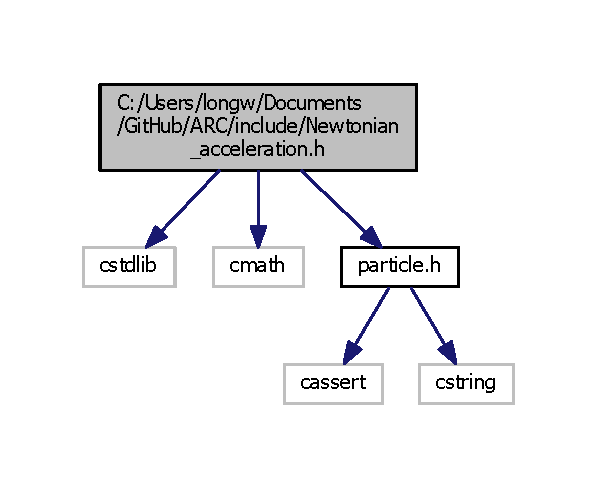
\includegraphics[width=287pt]{Newtonian__acceleration_8h__incl}
\end{center}
\end{figure}
\subsection*{Classes}
\begin{DoxyCompactItemize}
\item 
class \hyperlink{classNTA_1_1Newtonian__pars}{N\+T\+A\+::\+Newtonian\+\_\+pars}
\begin{DoxyCompactList}\small\item\em Newtonian Interaction and time transformation function parameter class. \end{DoxyCompactList}\end{DoxyCompactItemize}
\subsection*{Namespaces}
\begin{DoxyCompactItemize}
\item 
 \hyperlink{namespaceNTA}{N\+TA}
\begin{DoxyCompactList}\small\item\em Namespace for Newtonian Interaction related functions. \end{DoxyCompactList}\end{DoxyCompactItemize}
\subsection*{Functions}
\begin{DoxyCompactItemize}
\item 
int \hyperlink{namespaceNTA_a831c3f8f362f34f1f987ee158e38c016}{N\+T\+A\+::\+Newtonian\+\_\+\+AW} (double Aij\mbox{[}3\mbox{]}, double \&Pij, double p\+Wij\mbox{[}3\mbox{]}, double \&Wij, const double xij\mbox{[}3\mbox{]}, const \hyperlink{classParticle}{Particle} \&pi, const \hyperlink{classParticle}{Particle} \&pj, const Newtonian\+\_\+pars $\ast$pars)
\begin{DoxyCompactList}\small\item\em Newtonian acceleration and $\partial W_{ij}/\partial \mathbf{x}_i$ from particle j to particle i (function type of \hyperlink{}{A\+R\+C\+::pair\+\_\+\+AW}) \end{DoxyCompactList}\item 
void \hyperlink{namespaceNTA_ac086c632a4f16eddc70f023f269d9c94}{N\+T\+A\+::\+Newtonian\+\_\+\+Ap} (double Aij\mbox{[}3\mbox{]}, double \&Pij, const double xi\mbox{[}3\mbox{]}, const double xp\mbox{[}3\mbox{]}, const \hyperlink{classParticle}{Particle} \&pi, const \hyperlink{classParticle}{Particle} \&pp, const Newtonian\+\_\+pars $\ast$pars)
\begin{DoxyCompactList}\small\item\em Newtonian acceleration from particle p to particle i (function type of \+::\+A\+R\+C\+::pair\+\_\+\+Ap) \end{DoxyCompactList}\item 
double \hyperlink{namespaceNTA_a387c8276183c856f55e73a719977d437}{N\+T\+A\+::\+Newtonian\+\_\+kepler\+\_\+period} (const double m1, const double m2, const double dx\mbox{[}3\mbox{]}, const double dv\mbox{[}3\mbox{]}, const Newtonian\+\_\+pars $\ast$pars)
\begin{DoxyCompactList}\small\item\em Newtonian two-\/body kepler period. \end{DoxyCompactList}\item 
void \hyperlink{namespaceNTA_a02d22f02e21004b264c8257a5ffbb600}{N\+T\+A\+::calc\+\_\+kepler\+\_\+orbit\+\_\+par} (double \&semi, double \&peri, double \&ecc, double angle\mbox{[}3\mbox{]}, double \&true\+\_\+anomaly, double \&ecc\+\_\+anomaly, double \&mean\+\_\+anomaly, const double m, const double dx\mbox{[}3\mbox{]}, const double dv\mbox{[}3\mbox{]})
\begin{DoxyCompactList}\small\item\em Calculate parameters of two-\/body motion. \end{DoxyCompactList}\item 
void \hyperlink{namespaceNTA_a621b3643cd91a5a7ea23b7b22481f121}{N\+T\+A\+::kepler\+\_\+orbit\+\_\+generator} (double x1\mbox{[}3\mbox{]}, double x2\mbox{[}3\mbox{]}, double v1\mbox{[}3\mbox{]}, double v2\mbox{[}3\mbox{]}, const double m1, const double m2, const double semi, const double ecc, const double angle\mbox{[}3\mbox{]}, const double ecc\+\_\+anomaly)
\end{DoxyCompactItemize}

\hypertarget{particle_8h}{}\section{C\+:/\+Users/longw/\+Documents/\+Git\+Hub/\+A\+R\+C/include/particle.h File Reference}
\label{particle_8h}\index{C\+:/\+Users/longw/\+Documents/\+Git\+Hub/\+A\+R\+C/include/particle.\+h@{C\+:/\+Users/longw/\+Documents/\+Git\+Hub/\+A\+R\+C/include/particle.\+h}}
{\ttfamily \#include $<$cassert$>$}\newline
{\ttfamily \#include $<$cstring$>$}\newline
\subsection*{Classes}
\begin{DoxyCompactItemize}
\item 
class \hyperlink{classParticle}{Particle}
\begin{DoxyCompactList}\small\item\em A sample particle class used for \hyperlink{classARC_1_1chain}{A\+R\+C\+::chain}. \end{DoxyCompactList}\end{DoxyCompactItemize}
\subsection*{Macros}
\begin{DoxyCompactItemize}
\item 
\#define \hyperlink{particle_8h_a9914f6bd31eac2dedd31fb2d29f22ce2}{N\+A\+N\+\_\+\+C\+H\+E\+CK}(val)~assert((val) == (val));
\end{DoxyCompactItemize}


\subsection{Macro Definition Documentation}
\hypertarget{particle_8h_a9914f6bd31eac2dedd31fb2d29f22ce2}{}\label{particle_8h_a9914f6bd31eac2dedd31fb2d29f22ce2} 
\index{particle.\+h@{particle.\+h}!N\+A\+N\+\_\+\+C\+H\+E\+CK@{N\+A\+N\+\_\+\+C\+H\+E\+CK}}
\index{N\+A\+N\+\_\+\+C\+H\+E\+CK@{N\+A\+N\+\_\+\+C\+H\+E\+CK}!particle.\+h@{particle.\+h}}
\subsubsection{\texorpdfstring{N\+A\+N\+\_\+\+C\+H\+E\+CK}{NAN\_CHECK}}
{\footnotesize\ttfamily \#define N\+A\+N\+\_\+\+C\+H\+E\+CK(\begin{DoxyParamCaption}\item[{}]{val }\end{DoxyParamCaption})~assert((val) == (val));}


%--- End generated contents ---

% Index
\backmatter
\newpage
\phantomsection
\clearemptydoublepage
\addcontentsline{toc}{chapter}{Index}
\printindex

\end{document}
